\documentclass[10pt]{beamer}
\usepackage{graphicx}
\usepackage{adjustbox}
\usepackage{hyperref}
\usepackage{amsmath}
\usepackage{hyperref}
\usepackage{graphicx}
\usepackage{float}
\usepackage{caption}
\usepackage{listings}
\usepackage{xcolor}
\usepackage{multimedia}


\colorlet{punct}{red!60!black}
\definecolor{background}{RGB}{240, 248, 255}
\definecolor{delim}{RGB}{20,105,176}
\colorlet{numb}{magenta!60!black}

\lstdefinelanguage{json}{
    basicstyle=\ttfamily\footnotesize\color{black},
    numbers=left,
    numberstyle=\scriptsize,
    stepnumber=1,
    numbersep=8pt,
    showstringspaces=false,
    breaklines=true,
    frame=lines,
    backgroundcolor=\color{background},
    literate=
     *{0}{{{\color{numb}0}}}{1}
      {1}{{{\color{numb}1}}}{1}
      {2}{{{\color{numb}2}}}{1}
      {3}{{{\color{numb}3}}}{1}
      {4}{{{\color{numb}4}}}{1}
      {5}{{{\color{numb}5}}}{1}
      {6}{{{\color{numb}6}}}{1}
      {7}{{{\color{numb}7}}}{1}
      {8}{{{\color{numb}8}}}{1}
      {9}{{{\color{numb}9}}}{1}
      {:}{{{\color{punct}{:}}}}{1}
      {,}{{{\color{punct}{,}}}}{1}
      {\{}{{{\color{delim}{\{}}}}{1}
      {\}}{{{\color{delim}{\}}}}}{1}
      {[}{{{\color{delim}{[}}}}{1}
      {]}{{{\color{delim}{]}}}}{1},
}

\lstset{frame=single, showstringspaces=false, columns=fixed, basicstyle={\ttfamily}, commentstyle={\it}, numbers=left, tabsize=4}

\definecolor{codebackground}{RGB}{240, 248, 255}
\definecolor{codecomment}{RGB}{106,153,85}
\definecolor{codekeyword}{RGB}{30,30,255}
\definecolor{codestring}{RGB}{163,21,21}
\definecolor{codenumber}{RGB}{100,100,100}

\lstdefinestyle{modernstyle}{
    backgroundcolor=\color{codebackground},
    commentstyle=\color{codecomment},
    keywordstyle=\color{codekeyword},
    numberstyle=\tiny\color{codenumber},
    stringstyle=\color{codestring},
    basicstyle=\ttfamily\footnotesize\color{black},
    breakatwhitespace=false,
    breaklines=true,
    captionpos=b,
    keepspaces=true,
    numbers=left,
    numbersep=5pt,
    showspaces=false,
    showstringspaces=false,
    showtabs=false,
    tabsize=4
}

\lstset{style=modernstyle}

\usetheme{Copenhagen}
\usecolortheme{default}
\setbeamertemplate{navigation symbols}{}
\date{August 23, 2024}

\setbeamertemplate{footline}{%
  \leavevmode%
  \hbox{%
  \begin{beamercolorbox}[wd=.3\paperwidth,ht=2.25ex,dp=1ex,leftskip=.3cm plus1fil,rightskip=.3cm]{author in head/foot}%
    \usebeamerfont{author in head/foot}Giulio Carpi Lapi
  \end{beamercolorbox}%
  \begin{beamercolorbox}[wd=.3\paperwidth,ht=2.25ex,dp=1ex,center]{title in head/foot}%
    \usebeamerfont{title in head/foot}Exa-MA WP1 - Terrain
  \end{beamercolorbox}%
  \begin{beamercolorbox}[wd=.3\paperwidth,ht=2.25ex,dp=1ex,center]{institute in head/foot}%
    \usebeamerfont{institute in head/foot}M1 CSMI
  \end{beamercolorbox}%
  \begin{beamercolorbox}[wd=.1\paperwidth,ht=2.25ex,dp=1ex,rightskip=.3cm]{date in head/foot}%
    \usebeamerfont{date in head/foot}\insertframenumber{} / \inserttotalframenumber
  \end{beamercolorbox}}%
  \vskip0pt%
}



\title[Exa-MA WP1 - Terrain | Internship presentation]{
  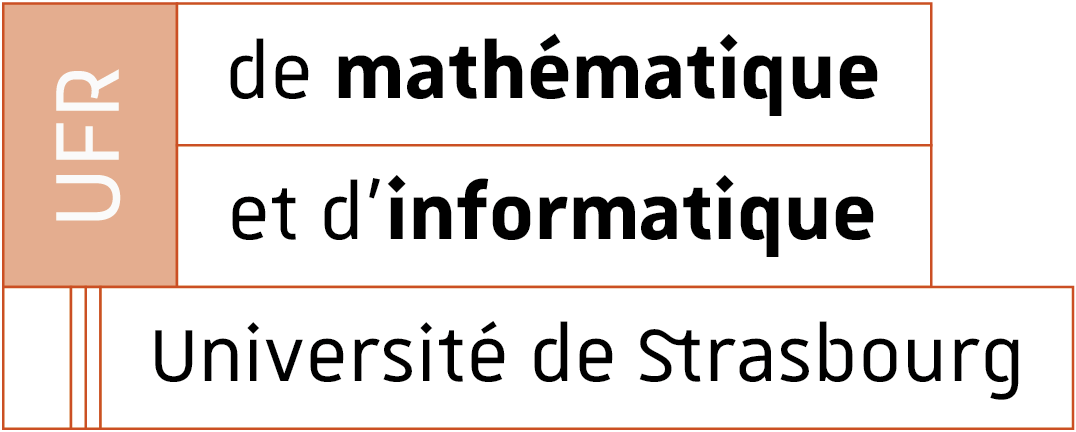
\includegraphics[width=0.8\textwidth]{images/logo-ufr.png}
  Exa-MA WP1 - Terrain}
\author[Giulio Carpi Lapi]{Giulio CARPI LAPI}

\begin{document}

\begin{frame}
  \titlepage
\end{frame}

\begin{frame}{Introduction}
  \begin{itemize}
    \Large
    \item Internship took place at \textbf{Cemosis - IRMA}
    \item \textbf{PEPR Numpex} through \textbf{Exa-MA} project
    \item Part of the \textbf{HiDALGO2} project
    \item \textbf{Ktirio Urban Building application}
    \item Supervised by \textbf{Vincent Chabannes}
  \end{itemize}
  \vfill
  \begin{figure}
    \centering
    \begin{minipage}{0.3\textwidth}
        \centering
        
\includegraphics[width=0.8\textwidth]{images/logo-cemosis.png}
        \captionsetup{font={scriptsize}}
        \caption{cemosis logo \cite{cemosis}}
    \end{minipage}
    \begin{minipage}{0.3\textwidth}
        \centering
        
\includegraphics[width=0.8\textwidth]{images/logo-numpex.png}
        \captionsetup{font={scriptsize}}
        \caption{Numpex logo \cite{numpex}}
    \end{minipage}
    \begin{minipage}{0.3\textwidth}
      \centering
      
\includegraphics[width=0.8\textwidth]{images/logo-hidalgo2.png}
      \captionsetup{font={scriptsize}}
      \caption{HiDALGO2 logo \cite{hidalgo2}}
    \end{minipage}
  \end{figure}
\end{frame}

\begin{frame}{Introduction: Main objectives}
  \begin{itemize}
    \Large
    \item \textbf{\textcolor{red}{Exa-MA WP1 - Terrain}}
    \vspace{1em}
    \item \textbf{Exa-MA WP1 - Vegetation}
    \item \textbf{Exa-MA WP1 - Urban Building LOD-1}
    \item \textbf{Exa-MA WP1 - Urban Building LOD-2}
    \vspace{2em}
    \item Develop a \textbf{\textcolor{red}{detailed 3D model}} of the urban landscape
  \end{itemize}
\end{frame}

\begin{frame}{Introduction: Main objectives}
  \Large
  \begin{itemize}
    \item Source elevation data from \textbf{Mapbox}
    \item \textbf{Reduce mesh density} with \textbf{contour line constraints}
    \item \textbf{Parallelization}
  \end{itemize}
\end{frame}

\begin{frame}{Introduction: Software and libraries}
  \Large
  \begin{figure}[H]
      \centering
      
\includegraphics[width=0.7\textwidth]{images/logo-nlohmann.png}
      \captionsetup{font={scriptsize}}
      \caption{json nlohmann logo\cite{json-nlohmann}}
  \end{figure}
  \begin{center}
    \Large C++ library for \textbf{JSON} parsing
  \end{center}
\end{frame}

\begin{frame}{Introduction: Software and libraries}
  \Large
  \begin{figure}[H]
      \centering
      
\includegraphics[width=0.6\textwidth]{images/logo-curl.png}
      \captionsetup{font={scriptsize}}
      \caption{curl logo\cite{curl}}
  \end{figure}
  \begin{center}
    \Large \textbf{URL} transfer library
  \end{center}
\end{frame}

\begin{frame}{Introduction: Software and libraries}
  \Large
  \begin{figure}[H]
      \centering
      
\includegraphics[width=0.4\textwidth]{images/logo-libpng.png}
      \captionsetup{font={scriptsize}}
      \caption{libpng logo\cite{libpng}}
  \end{figure}
  \begin{center}
    \Large \textbf{PNG} reference library
  \end{center}
\end{frame}

\begin{frame}{Introduction: Software and libraries}
  \Large
  \begin{figure}[H]
      \centering
      
\includegraphics[width=0.8\textwidth]{images/logo-cgal.png}
      \captionsetup{font={scriptsize}}
      \caption{CGAL logo\cite{cgal}}
  \end{figure}
  \begin{center}
    \Large Open source software library for \textbf{computational geometry algorithms}
  \end{center}
\end{frame}

\begin{frame}{Methodology: Pre-existing codebase}
  \begin{figure}[H]
    \centering
    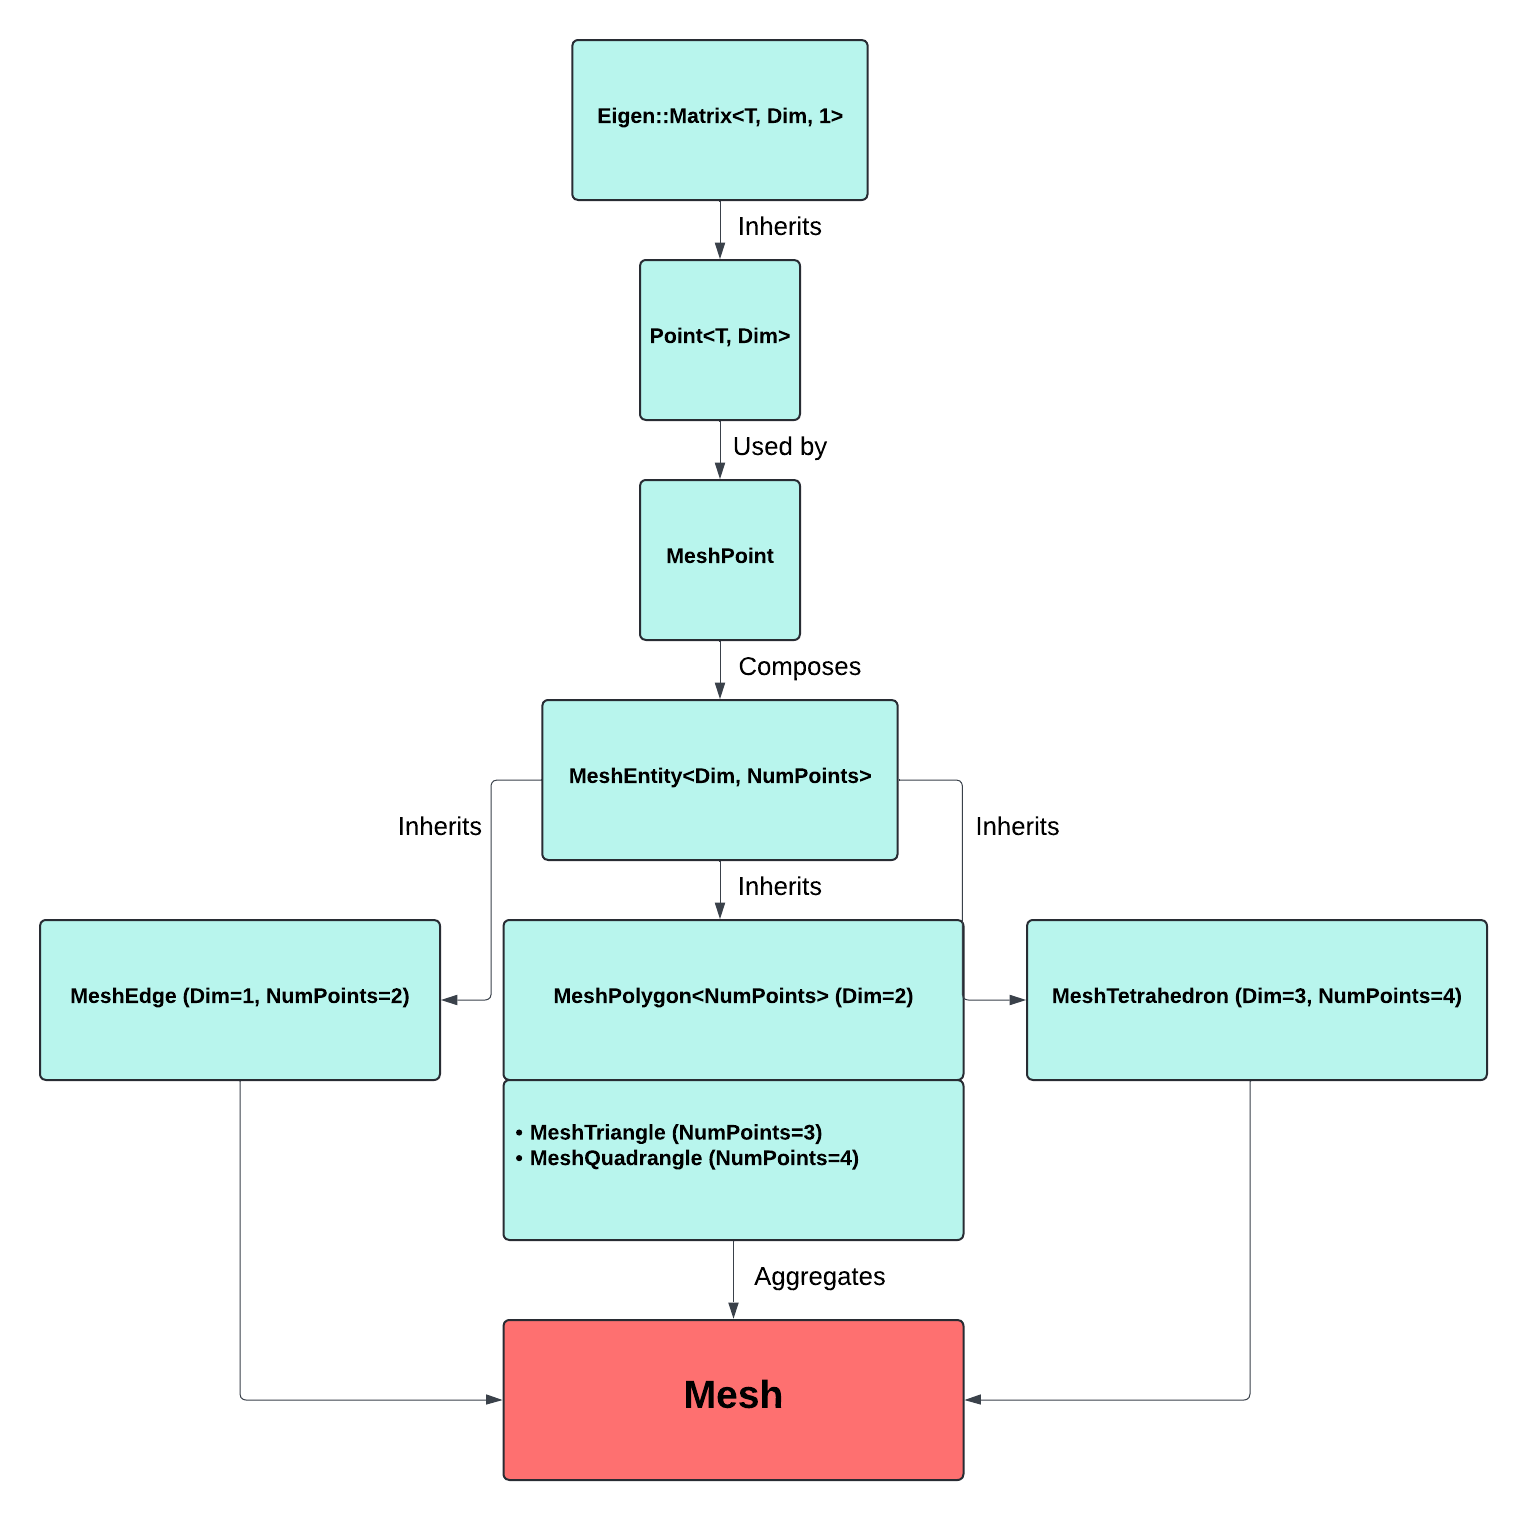
\includegraphics[width=0.7\textwidth]{images/uml-codebase-1.png}
    \captionsetup{font={scriptsize}}
    \caption{UML diagram of the codebase structure 1}
  \end{figure}
\end{frame}

\begin{frame}{Methodology: Pre-existing codebase}
  \begin{figure}[H]
    \centering
    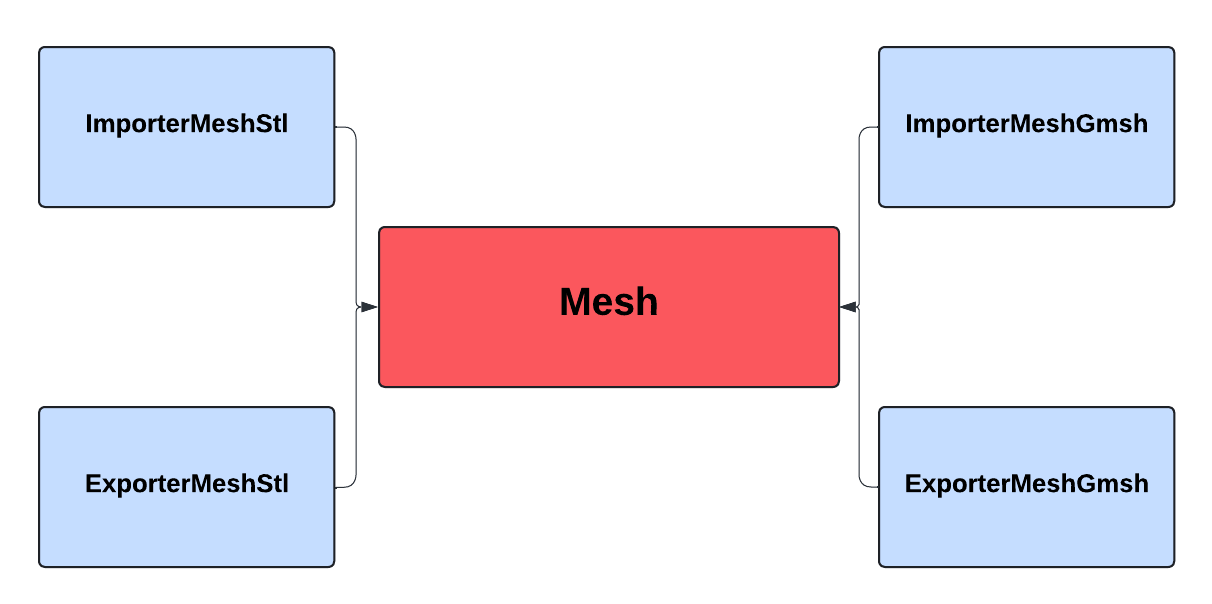
\includegraphics[width=0.8\textwidth]{images/uml-codebase-2.png}
    \captionsetup{font={scriptsize}}
    \caption{UML diagram of the codebase structure 2}
  \end{figure}
\end{frame}

\begin{frame}[fragile]{Methodology: Configuration}
  \begin{lstlisting}[language=json]
{
  "useGPS": true,
  "precision": 0.5,
  "longitude": 5.7232,
  "latitude": 45.1835,
  "zoom": 16,
  "api_key": "[YOUR_API_KEY_HERE]"
}
  \end{lstlisting}
\end{frame}

\begin{frame}{Methodology: Latitude and longitude}
  \begin{figure}[H]
    \centering
    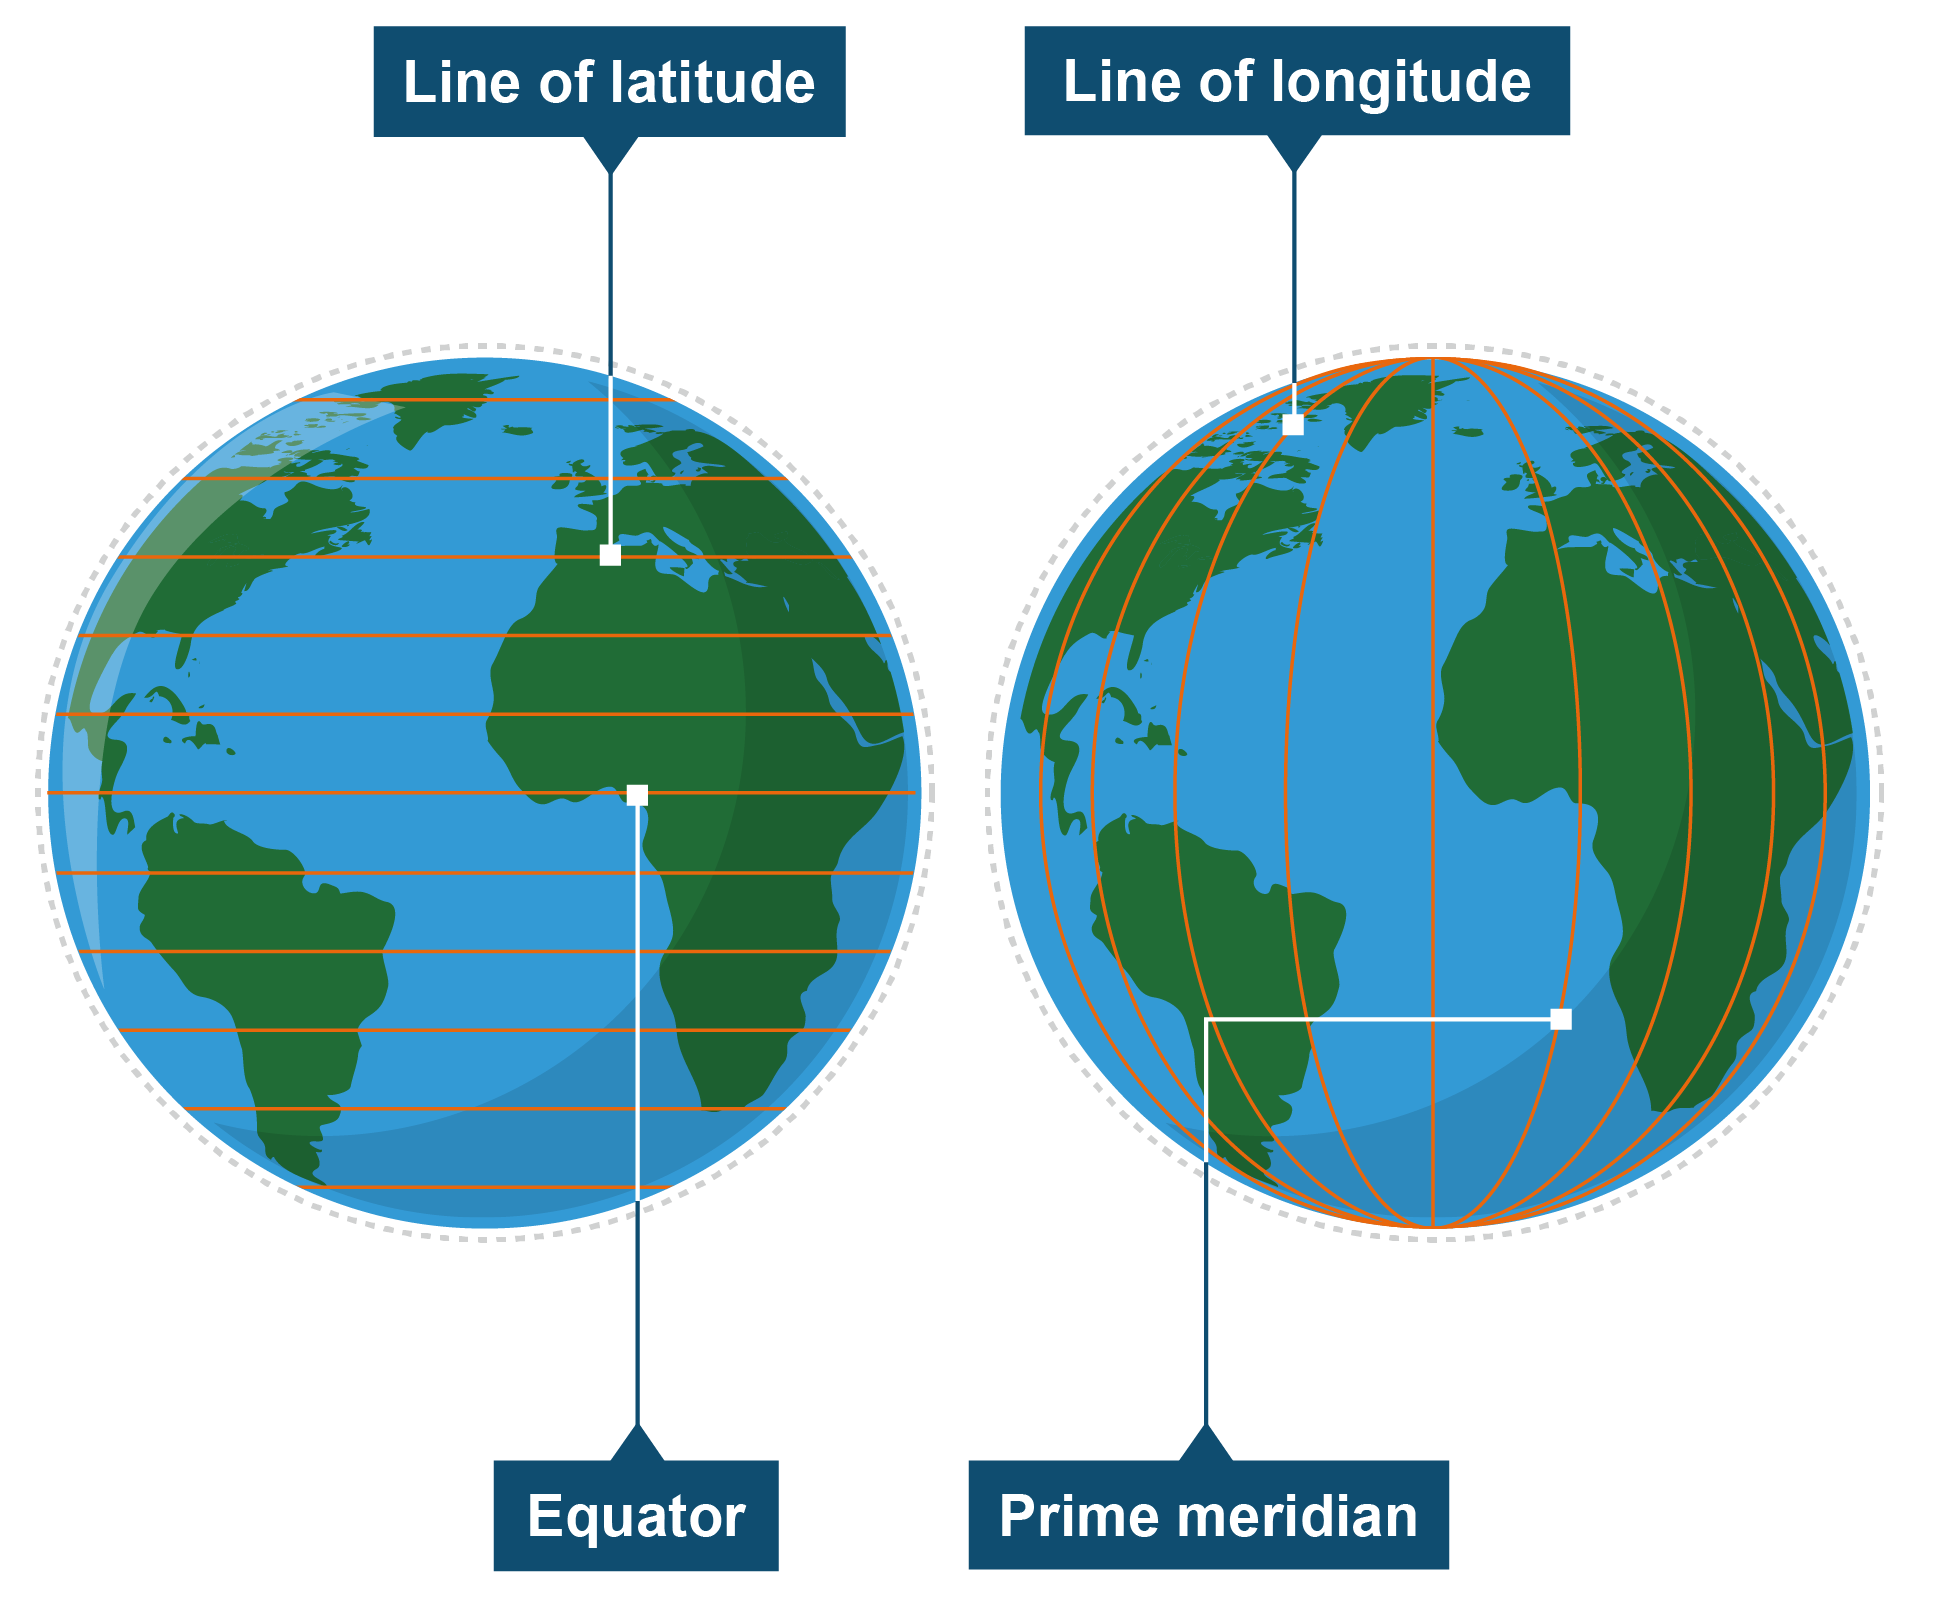
\includegraphics[width=0.7\textwidth]{images/lat-long.png}
    \captionsetup{font={scriptsize}}
    \caption{Latitude and longitude \cite{img:lat-lon}}
  \end{figure}
\end{frame}

\begin{frame}{Methodology: Mercator projection}
  \begin{figure}[H]
    \centering
    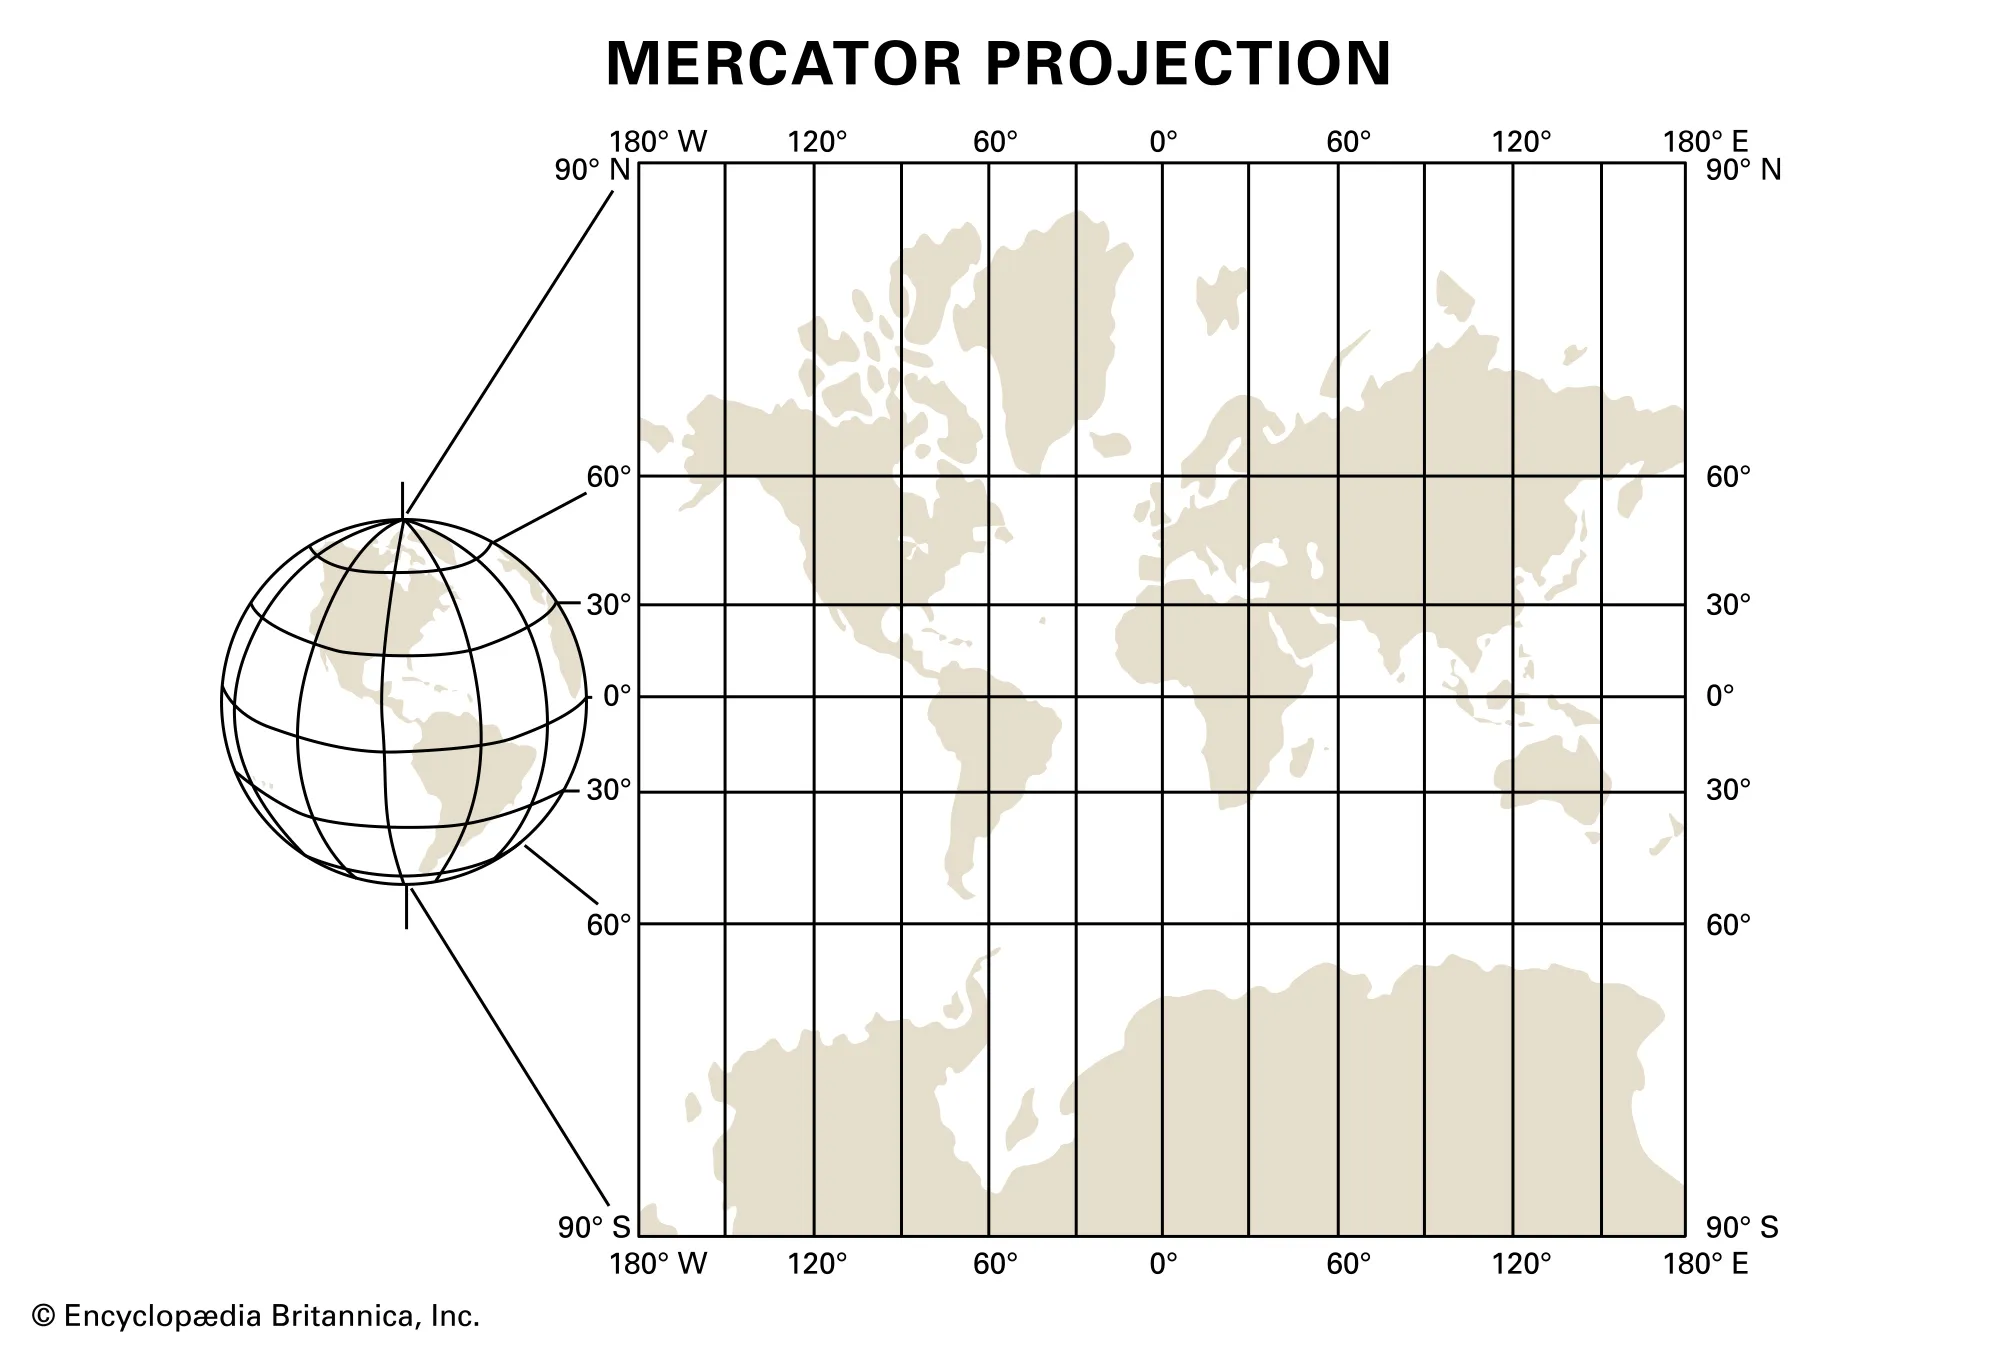
\includegraphics[width=0.7\textwidth]{images/mercator.png}
    \captionsetup{font={scriptsize}}
    \caption{Mercator projection \cite{img:mercator}}
  \end{figure}
\end{frame}

\begin{frame}{Methodology: Tiled web map}
  \begin{figure}[H]
    \centering
    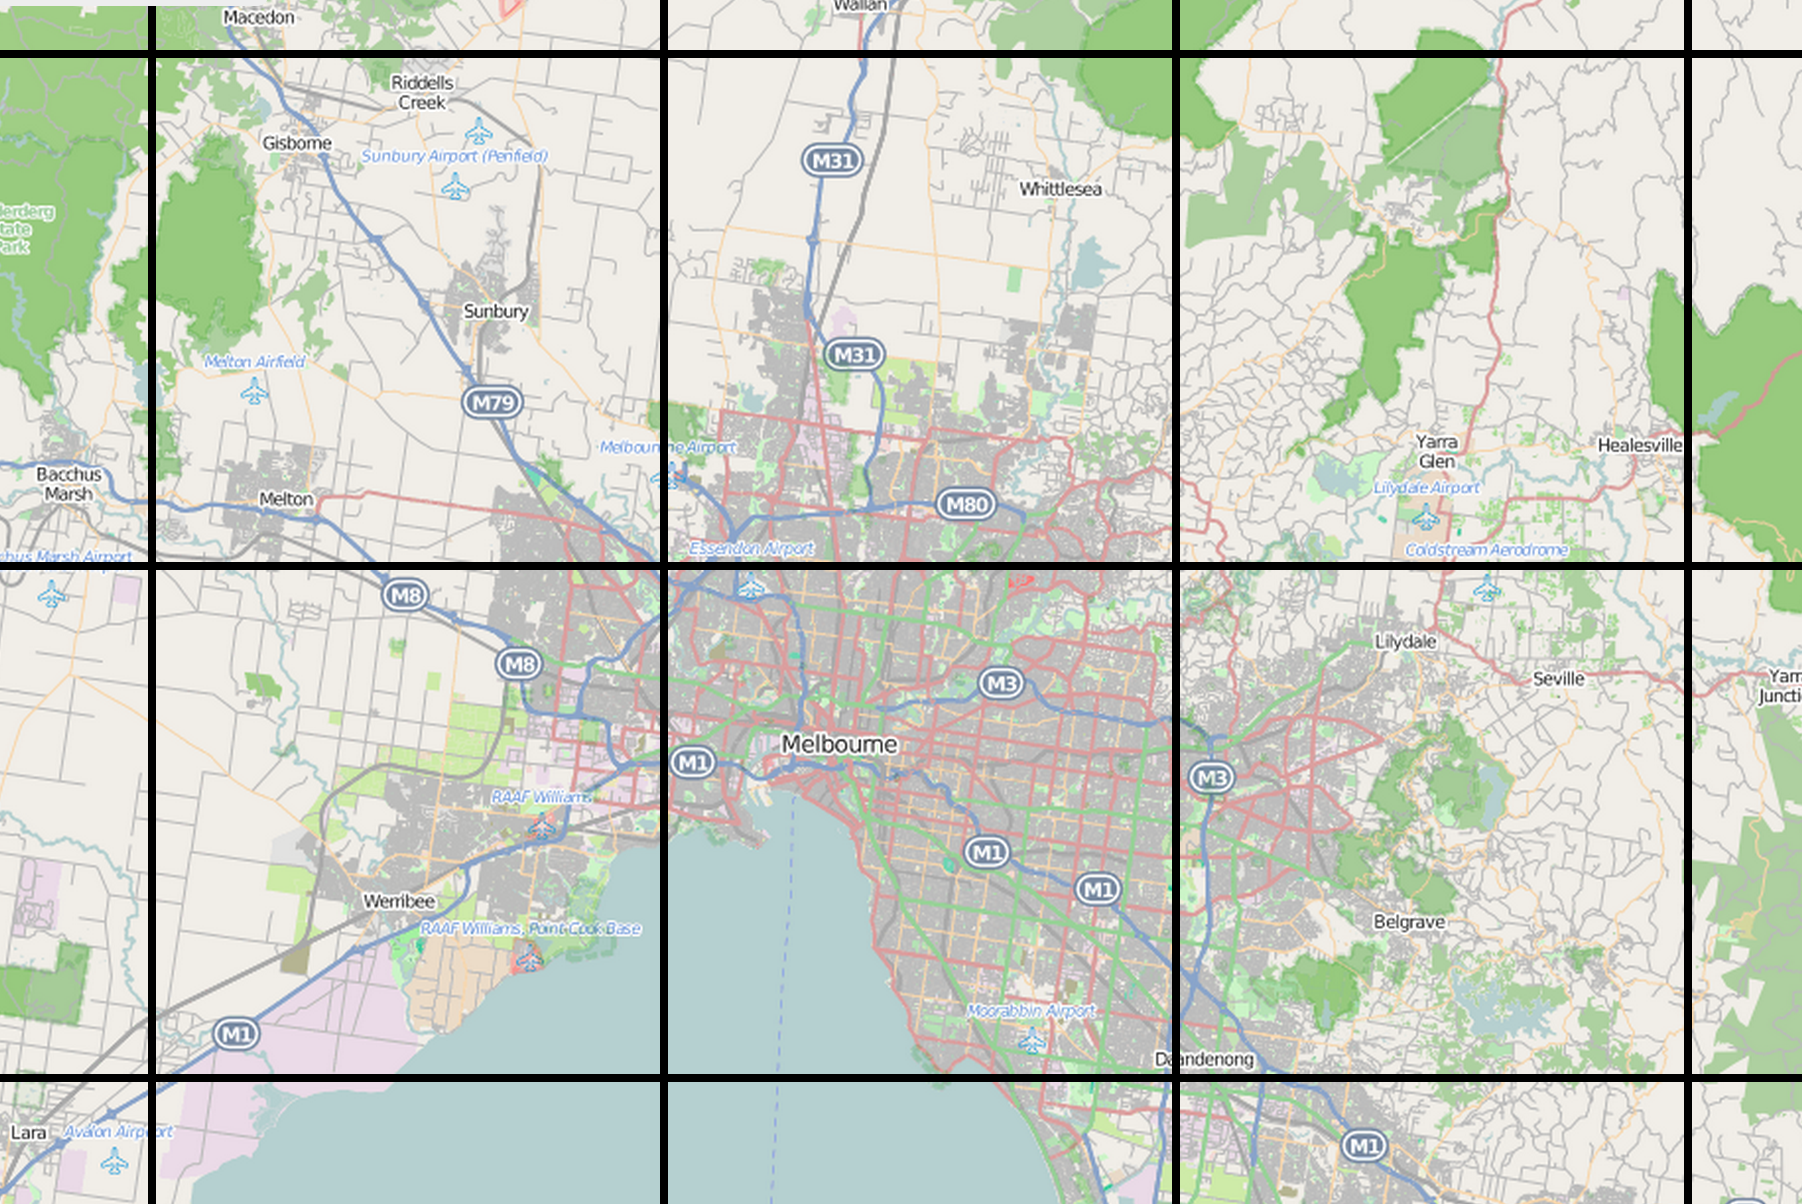
\includegraphics[width=0.8\textwidth]{images/tiled-web-map.png}
    \captionsetup{font={scriptsize}}
    \caption{Tiled web map \cite{img:tiled-web-map}}
  \end{figure}
\end{frame}

\begin{frame}{Methodology: Tiles coordinates}
  \begin{figure}[H]
    \centering
    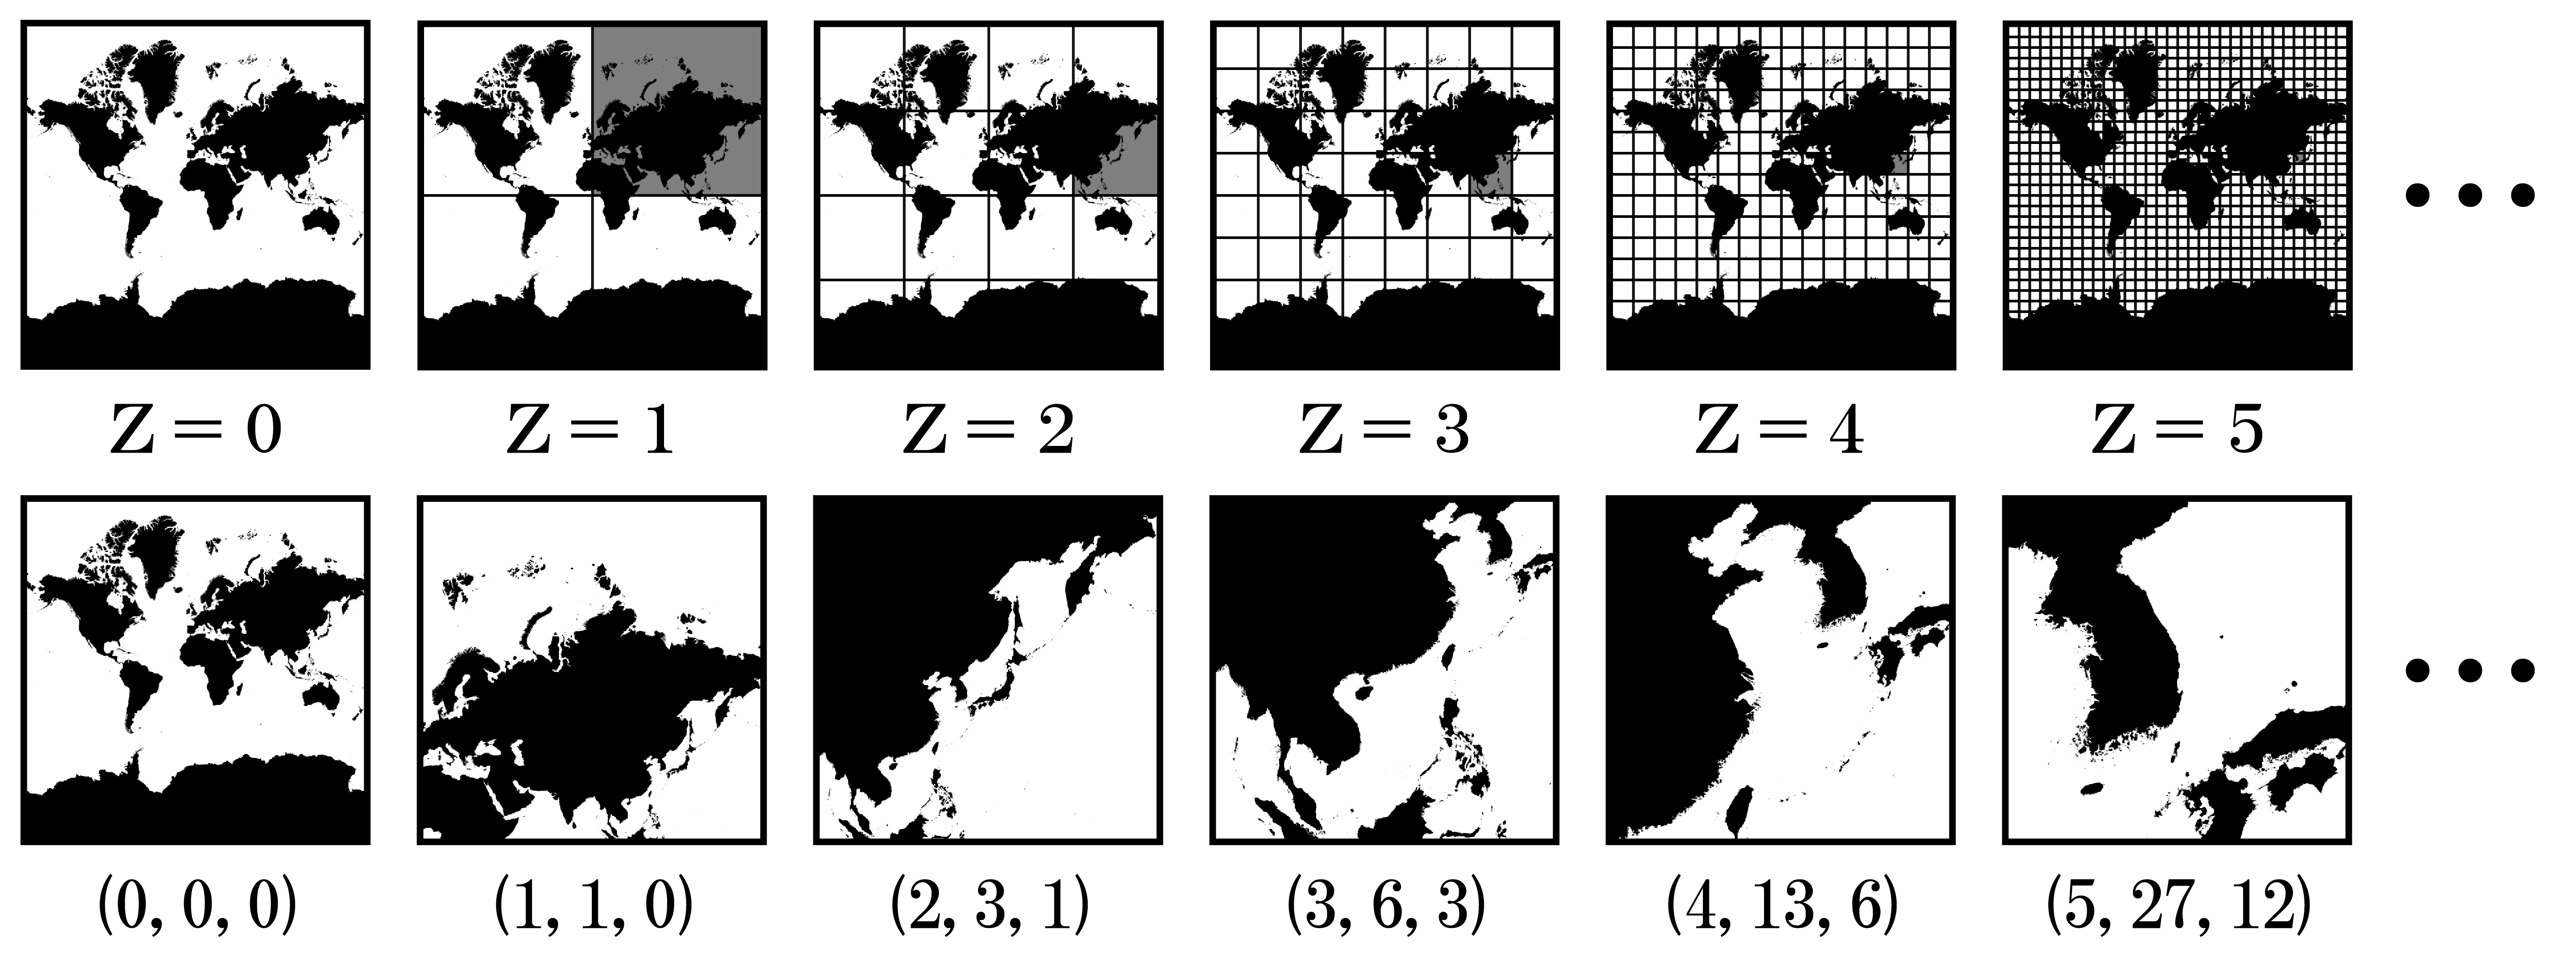
\includegraphics[width=0.9\textwidth]{images/tiles-coordinates.png}
    \captionsetup{font={scriptsize}}
    \caption{Tiles coordinates \cite{img:tiles-coordinates}}
  \end{figure}
\end{frame}

\begin{frame}[fragile]{Methodology: Data acquisition}
  \Large
  URL structure for \textbf{Mapbox Terrain-RGB v1} API:
  \vspace{2em}
  \begin{lstlisting}[language=C++]
"https://api.mapbox.com/v4/mapbox.terrain-rgb/" + std::to_string(zoom) + "/" + std::to_string(x) + "/" + std::to_string(y) + ".png?access_token=" + api_key;
  \end{lstlisting}
\end{frame}

\begin{frame}{Methodology: Geographic coordinates to tile coordinate}
  \Large
  \[
  x = \left\lfloor
    \frac{\text{lon} + 180}{360} \times 2^{\text{zoom}}
  \right\rfloor
  \]
  \vspace{1em}
  \[
  y = \left\lfloor
    \left(1 -
        \frac{
            \log\left(
                \tan\left(\frac{\text{lat} \times \pi}{180}\right) + 
                \frac{1}{\cos\left(\text{lat} \times \frac{\pi}{180}\right)}
            \right)
        }{\pi}
    \right) \times 2^{\text{zoom}}
  \right\rfloor
  \]
\end{frame}

\begin{frame}[fragile]{Methodology: Data acquisition}
  \Large
  Function to read PNG data:
  \vspace{1em}
  \begin{lstlisting}[language=C++]
std::vector<std::vector<std::tuple<int, int, int>>> readPNG(const std::vector<char> &data)
{
  std::vector<std::vector<std::tuple<int, int, int>>> image;
  std::vector<std::tuple<int, int, int>> row;
  for (unsigned x = 0; x < image_struct.width; ++x)
  {
      int r = buffer[3 * (y * image_struct.width + x) + 0];
      int g = buffer[3 * (y * image_struct.width + x) + 1];
      int b = buffer[3 * (y * image_struct.width + x) + 2];
      row.emplace_back(r, g, b);
  }
    return image;
}
  \end{lstlisting}
\end{frame}

\begin{frame}{Methodology: Mapbox Terrain-RGB v1}
  \Large
  \[
  height = -10000 + ((R \times 256 \times 256 + G \times 256 + B) \times 0.1)
  \]
\end{frame}

\begin{frame}{Methodology: Delaunay triangulation}
  \Large
  \begin{figure}[H]
    \centering
    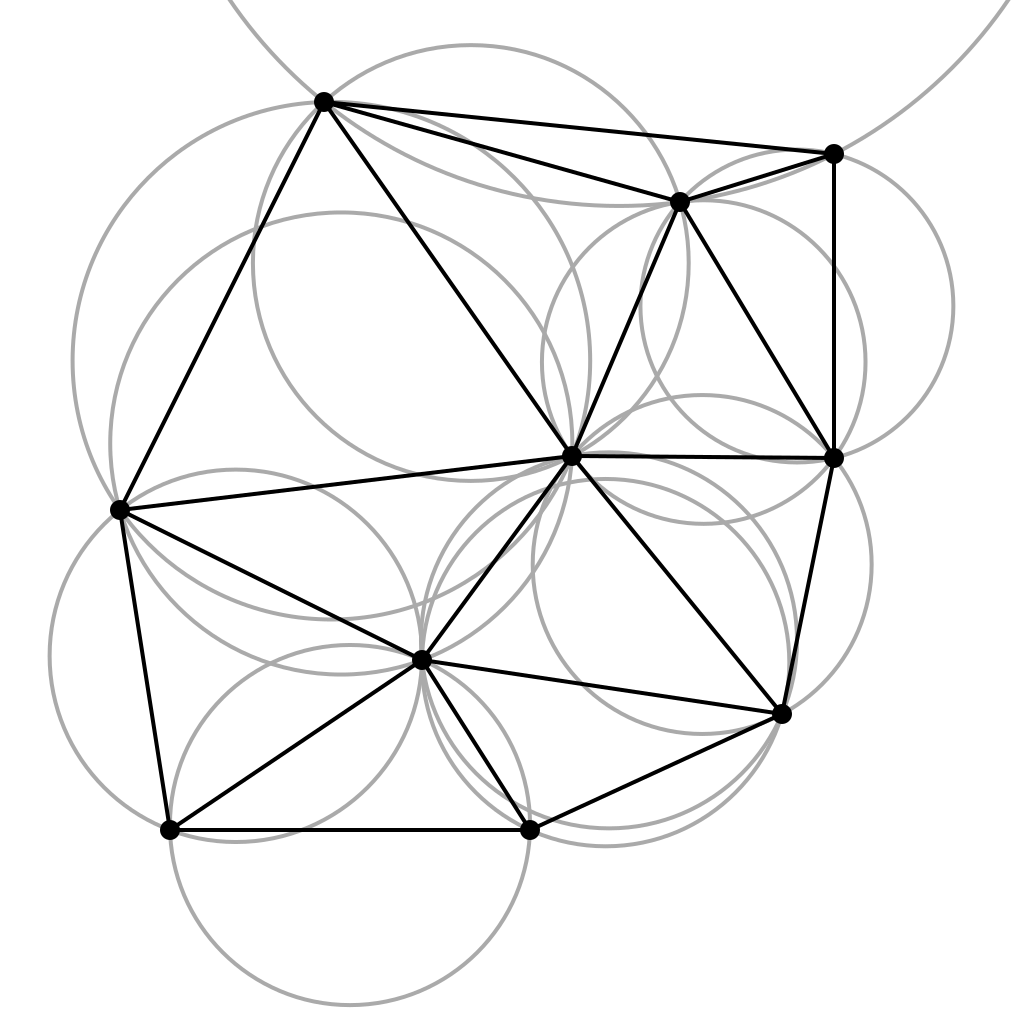
\includegraphics[width=0.6\textwidth]{images/delaunay-triangulation.png}
    \captionsetup{font={scriptsize}}
    \caption{Delaunay triangulation \cite{img:dt}}
\end{figure}
\end{frame}

\begin{frame}{Methodology: Constrained Delaunay triangulation}
  \Large
  \begin{figure}[H]
    \centering
    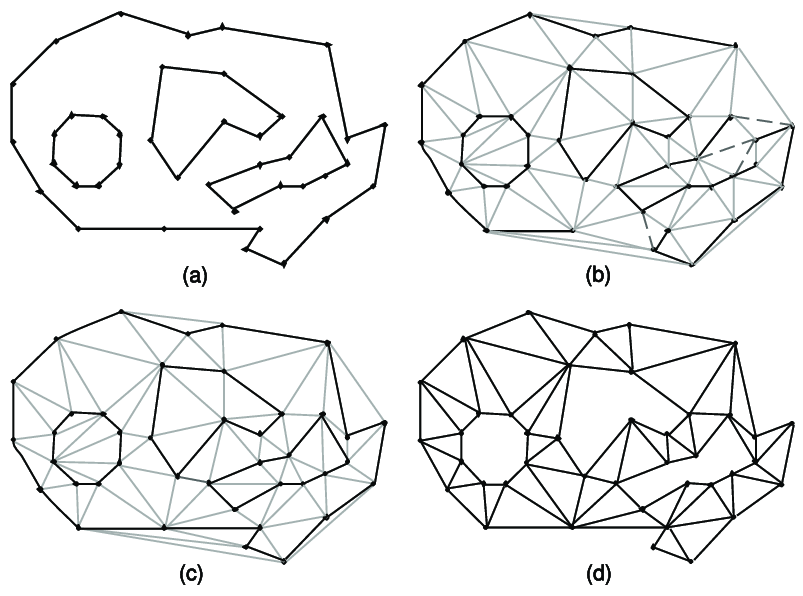
\includegraphics[width=0.8\textwidth]{images/constrained-delaunay-triangulation.png}
    \captionsetup{font={scriptsize}}
    \caption{Constrained Delaunay triangulation \cite{img:cdt}}
\end{figure}
\end{frame}

\begin{frame}{Implementation: Project structure}
  \begin{figure}[H]
    \centering
    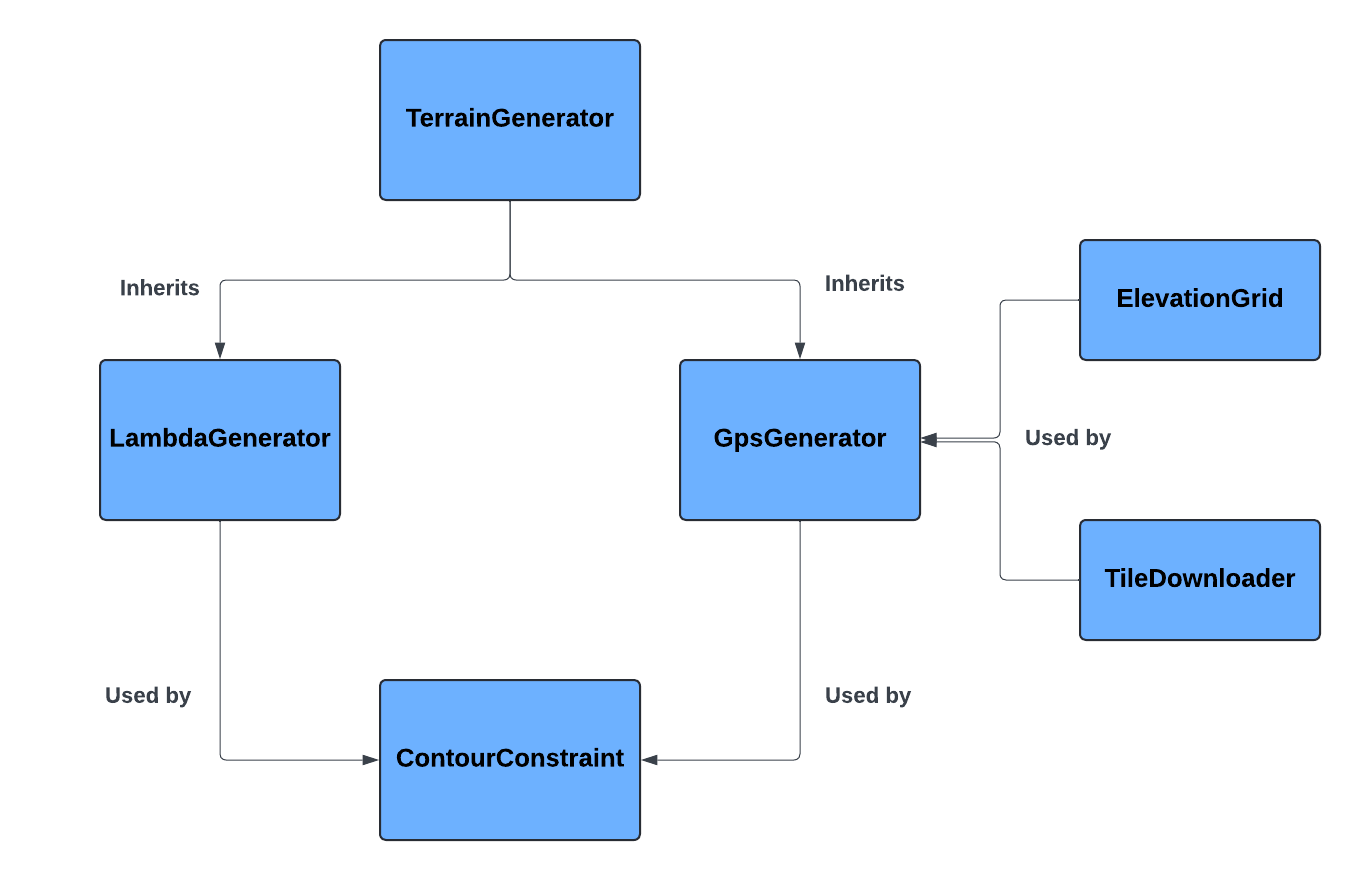
\includegraphics[width=0.9\textwidth]{images/uml-structure.png}
    \captionsetup{font={scriptsize}}
    \caption{UML diagram of the project structure}
  \end{figure}
\end{frame}

\begin{frame}[fragile]{Implementation: Mesh generation}
  \Large
  \textbf{TerrainGenerator} class definition:
  \vspace{2em}
  \begin{lstlisting}[language=C++]
class TerrainGenerator
{
public:
    using mesh_type = Mesh;
    virtual std::unique_ptr<mesh_type> generate() = 0;
    virtual ~TerrainGenerator() {};
};
  \end{lstlisting}
\end{frame}

\begin{frame}[fragile]{Implementation: Mesh generation}
  \Large
  \textbf{LambdaGenerator} class definition:
  \vspace{1em}
  \begin{lstlisting}[language=C++]
class LambdaGenerator : public TerrainGenerator
{
public:
    using fn_type = std::function<double(double, double)>;
    LambdaGenerator(int meshSize, fn_type const &fn);
    virtual ~LambdaGenerator();

    std::unique_ptr<mesh_type> generate() override;

private:
    int M_meshSize;
    fn_type M_fn;
};
  \end{lstlisting}
\end{frame}

\begin{frame}{Implementation: Mesh generation}
  \Large
    \[
    z(x, y) = \sqrt{r^2 - (x - x_0)^2 - (y - y_0)^2}
    \]
  \begin{figure}[H]
      \centering
      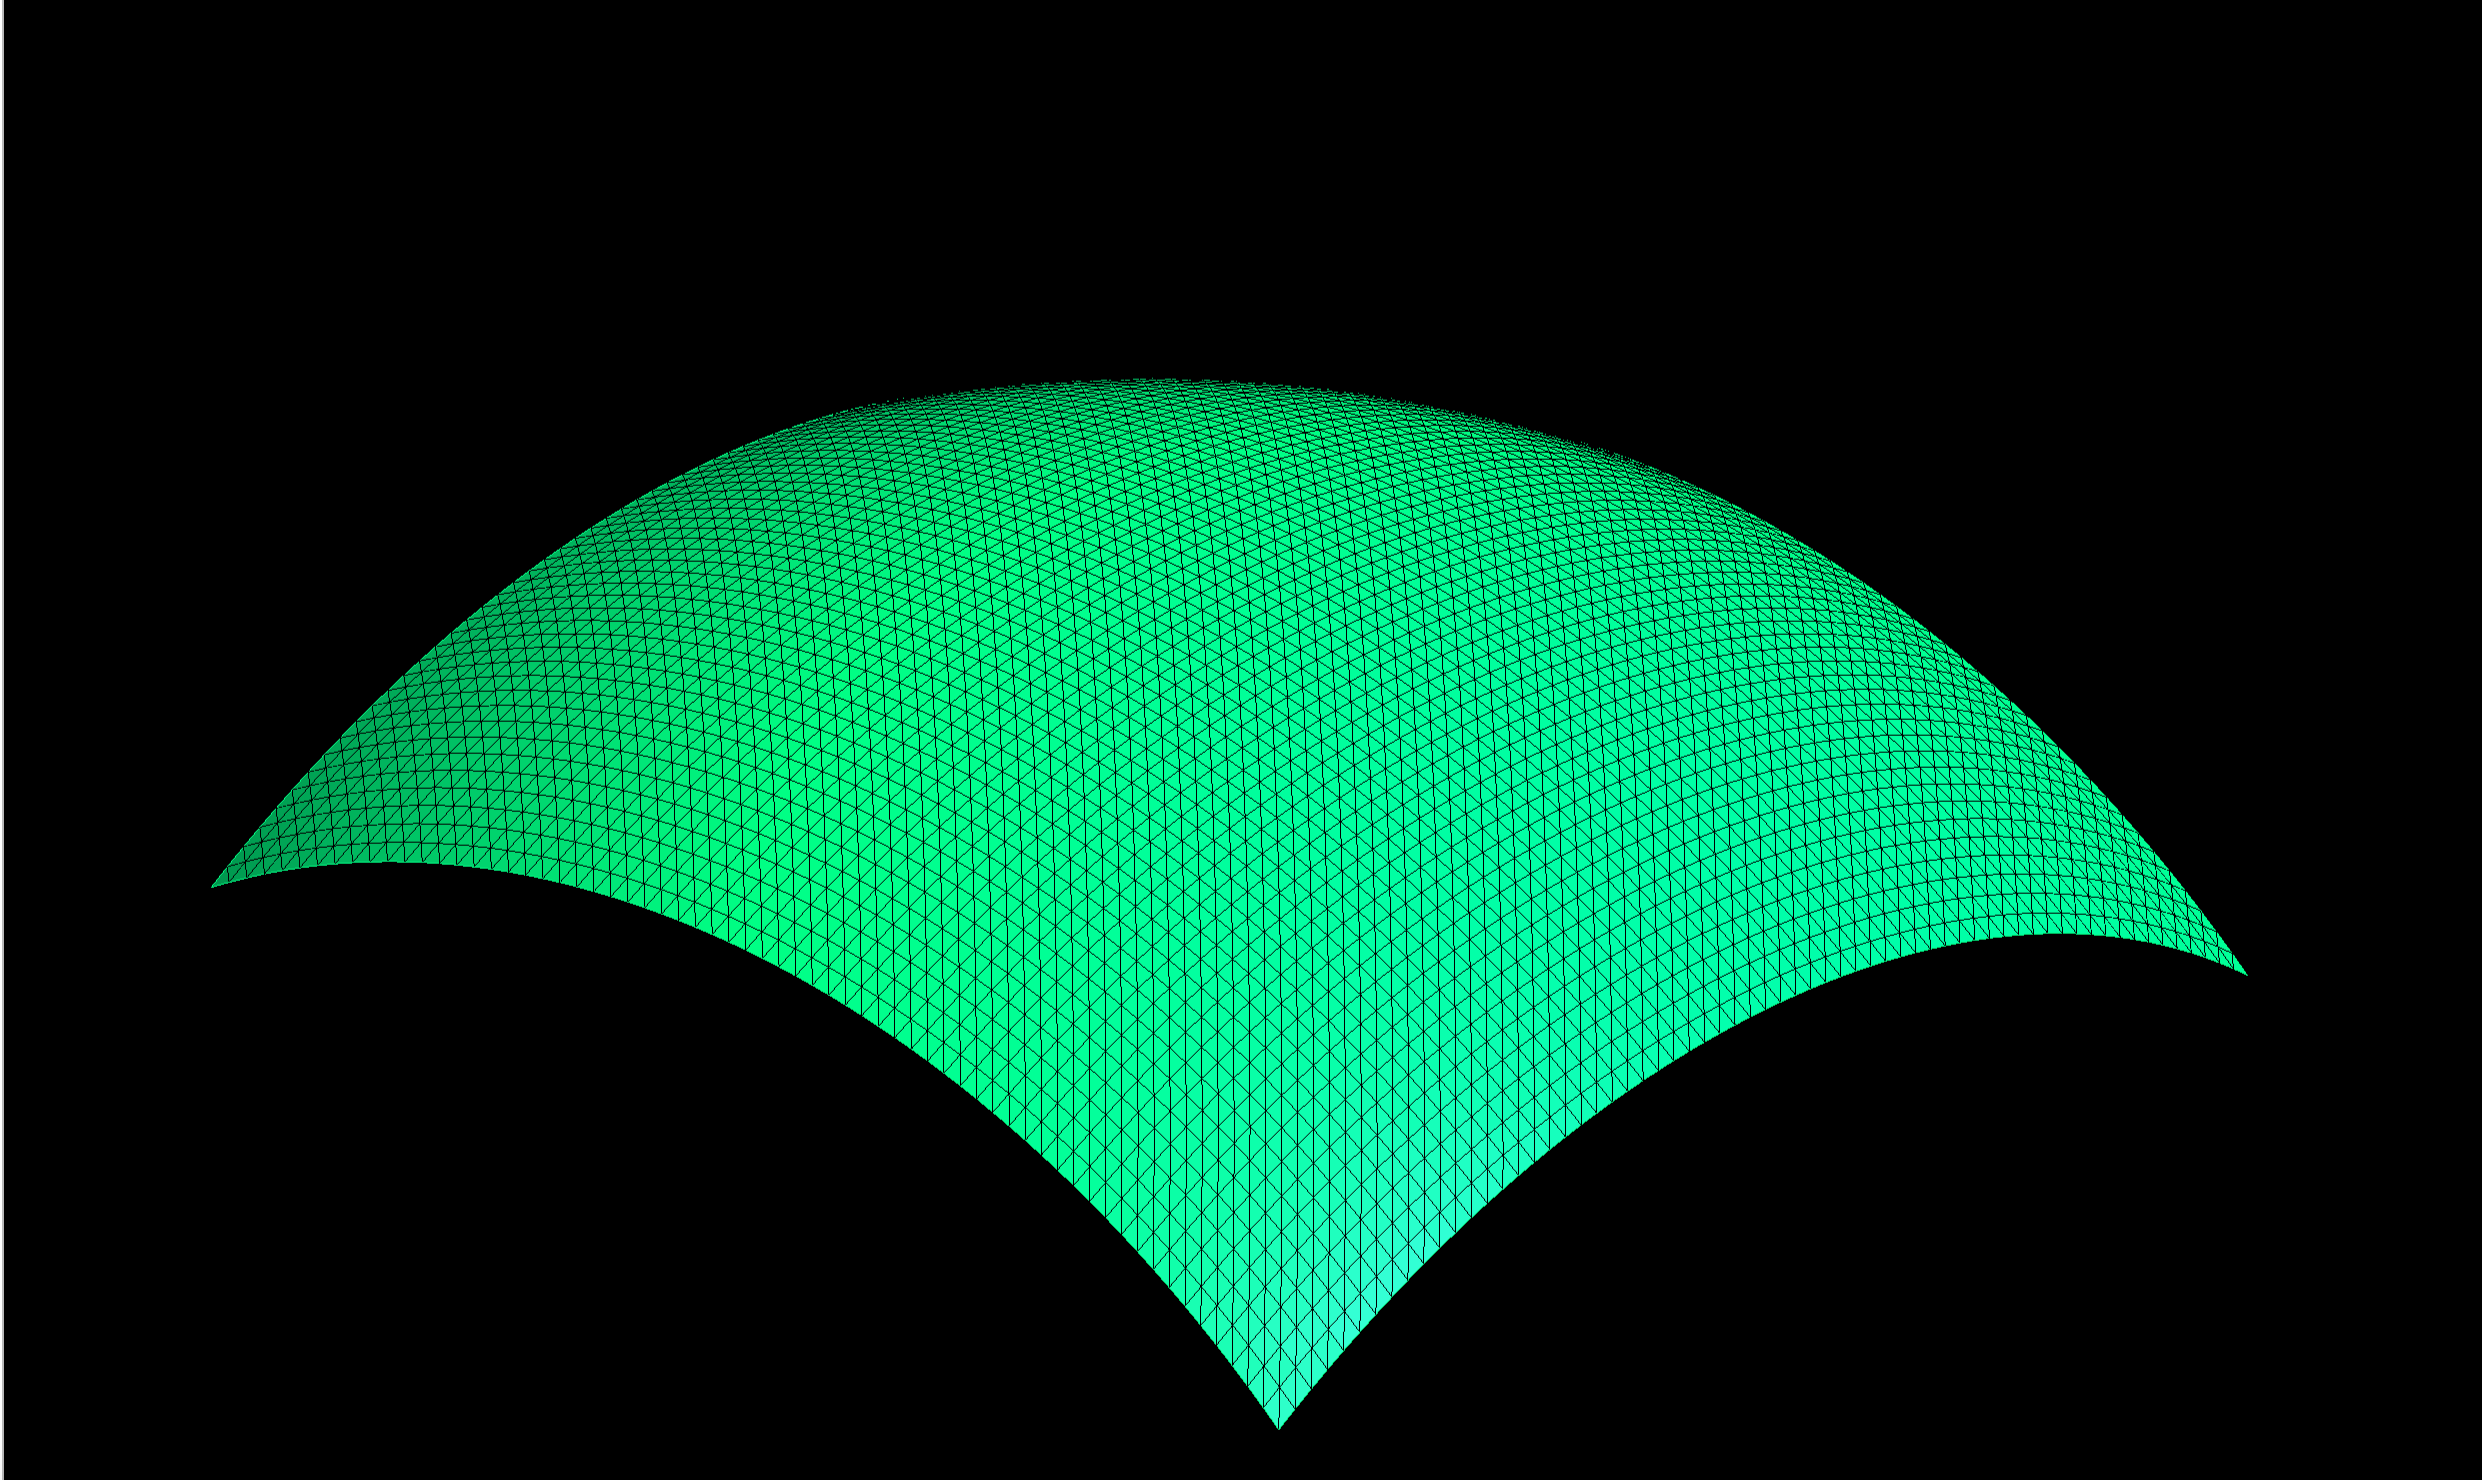
\includegraphics[width=0.8\textwidth]{images/generated-lambda-1.png}
      \captionsetup{font={scriptsize}}
      \caption{3D mesh \textbf{LambdaGenerator} 1}
  \end{figure}
\end{frame}

\begin{frame}{Implementation: Mesh generation}
  \Large
    \[
    z(x, y) = sin(x) + cos(y)
    \]
  \begin{figure}[H]
      \centering
      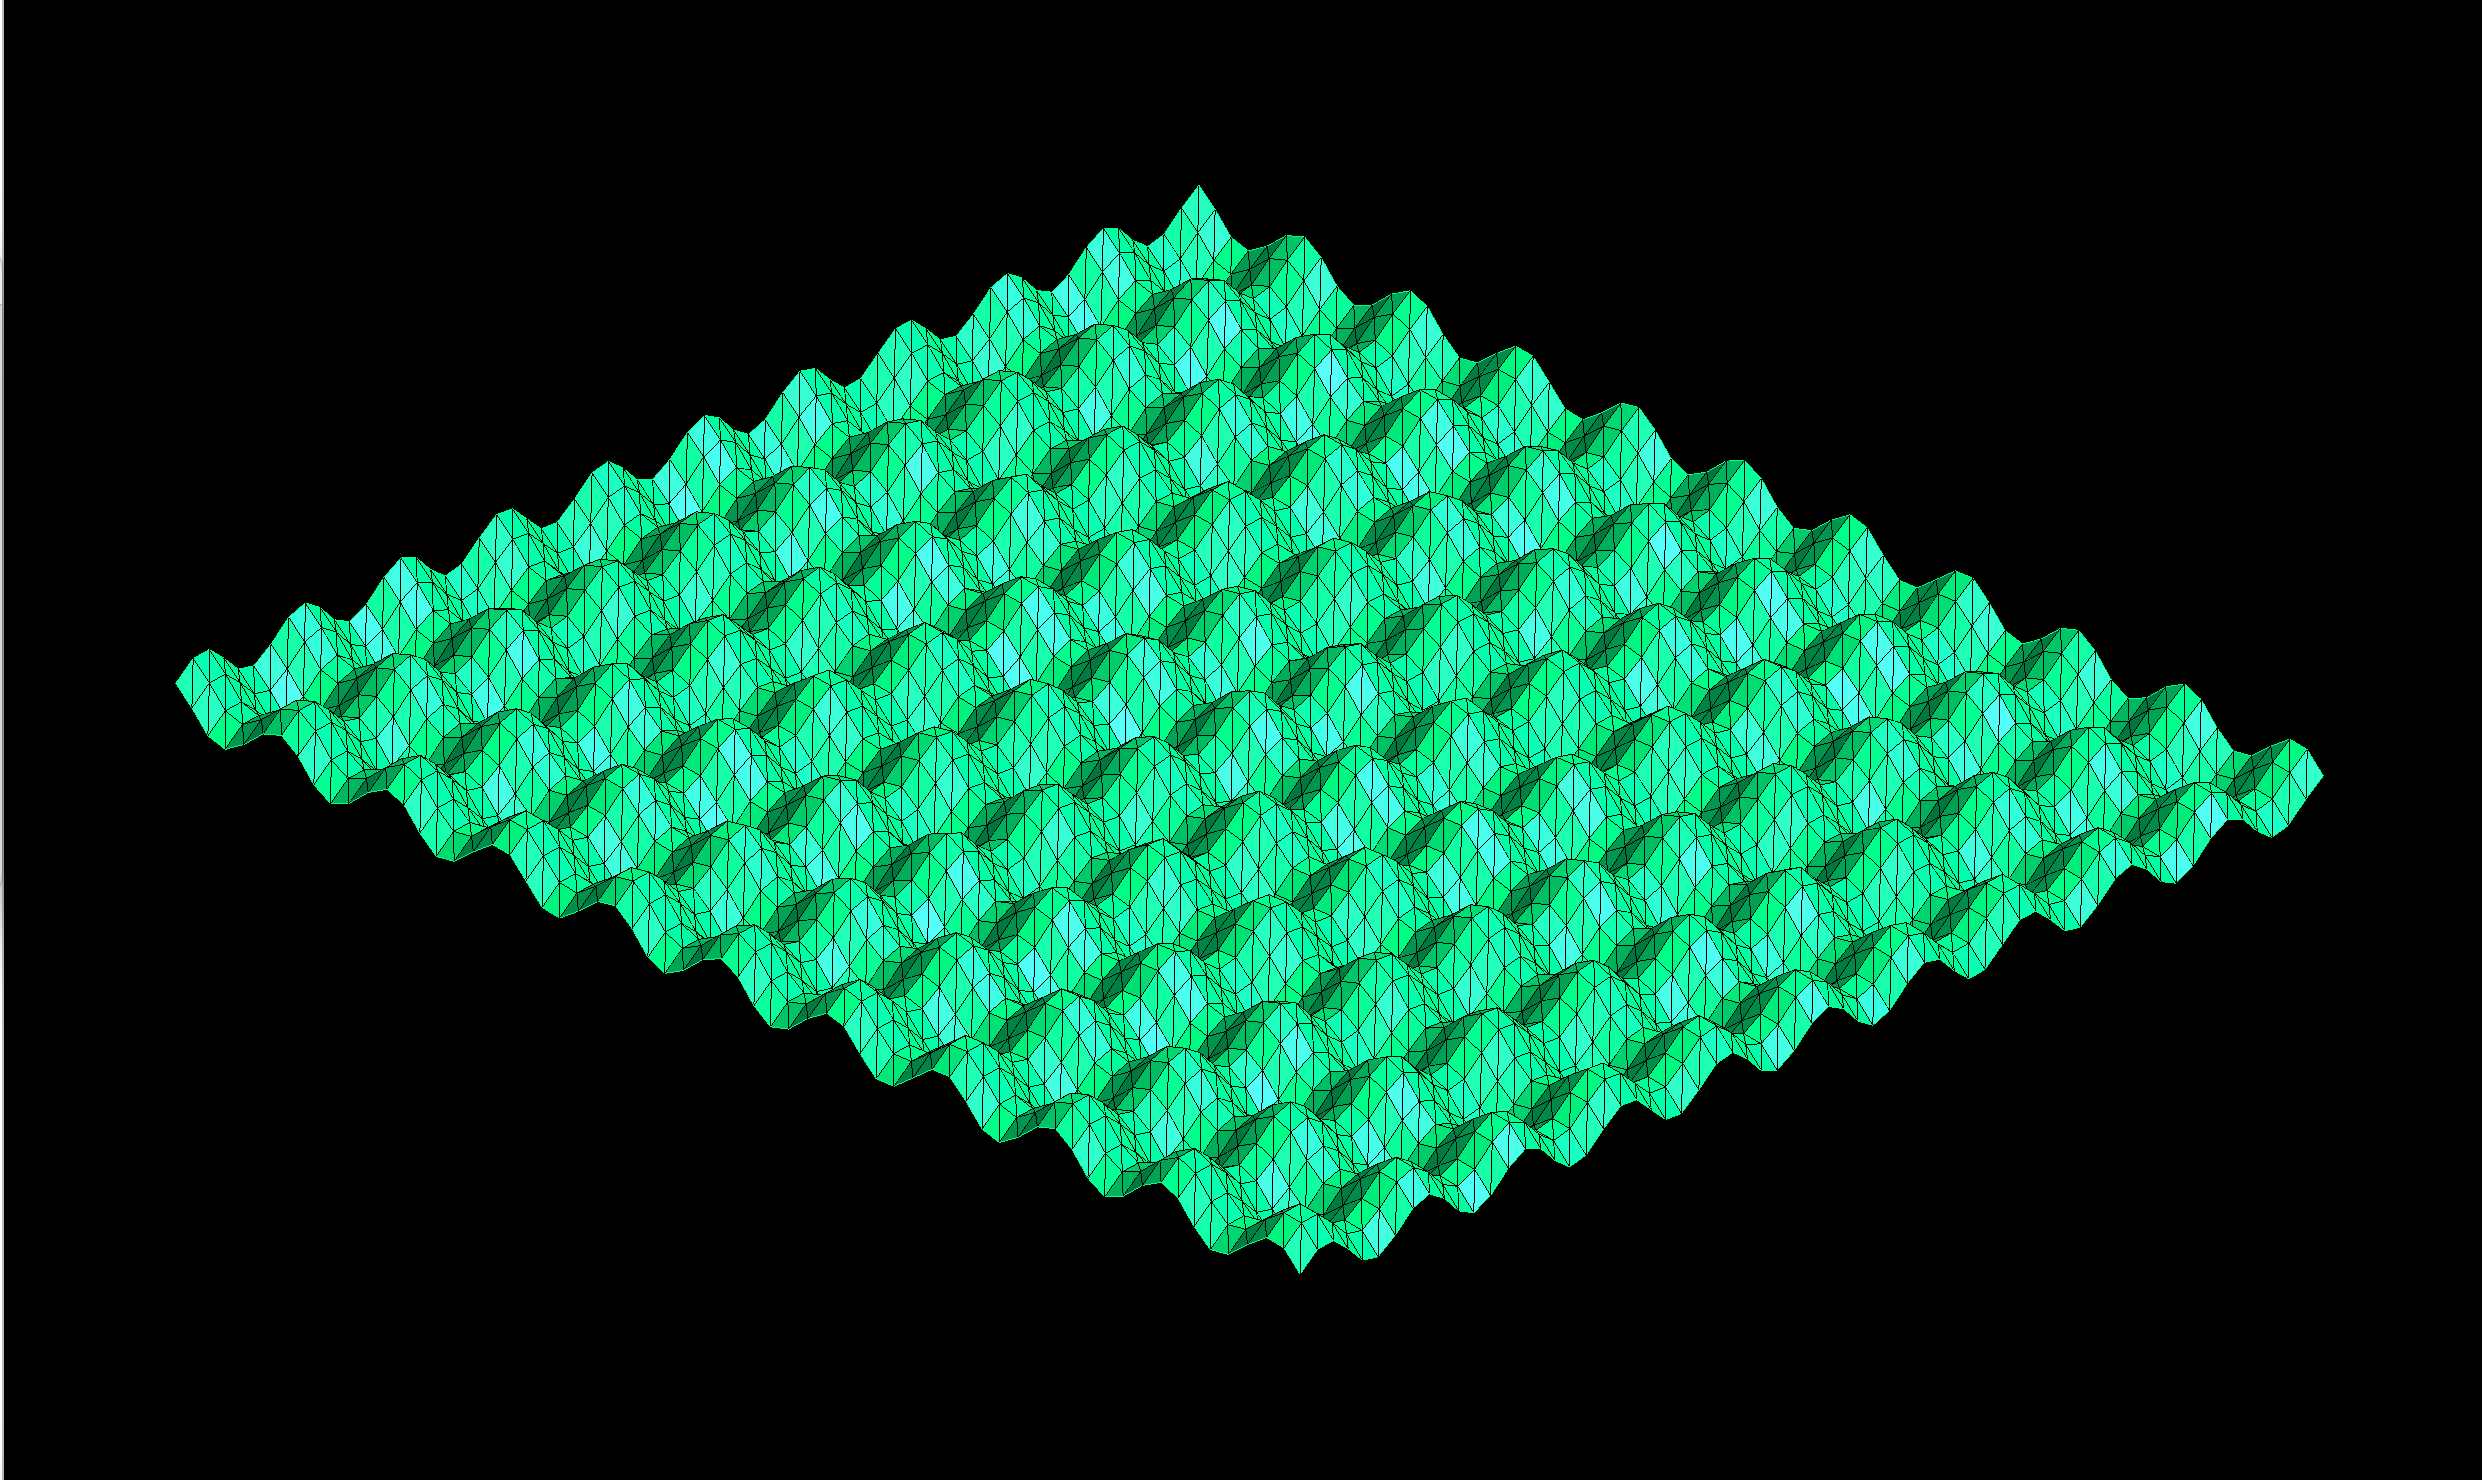
\includegraphics[width=0.8\textwidth]{images/generated-lambda-2.png}
      \captionsetup{font={scriptsize}}
      \caption{3D mesh \textbf{LambdaGenerator} 2}
  \end{figure}
\end{frame}

\begin{frame}[fragile]{Implementation: Mesh generation}
  \Large
  \textbf{GpsGenerator} class definition:
  \vspace{1em}
  \begin{lstlisting}[language=C++]
class GpsGenerator : public TerrainGenerator
{
public:
    GpsGenerator(int meshSize, double latitude, double longitude, unsigned zoomLevel, std::string const &apiKey);
    virtual ~GpsGenerator();

    std::unique_ptr<mesh_type> generate() override;

private:
    int M_meshSize;
    double M_latitude;
    double M_longitude;
    unsigned M_zoomLevel;
    std::string M_apiKey;
};
  \end{lstlisting}
\end{frame}

\begin{frame}{Implementation: Mesh generation}
  \centering
  \Large
  $(x, y) = (33809, 23527)$ at zoom level $16$
  \begin{figure}[H]
      \centering
      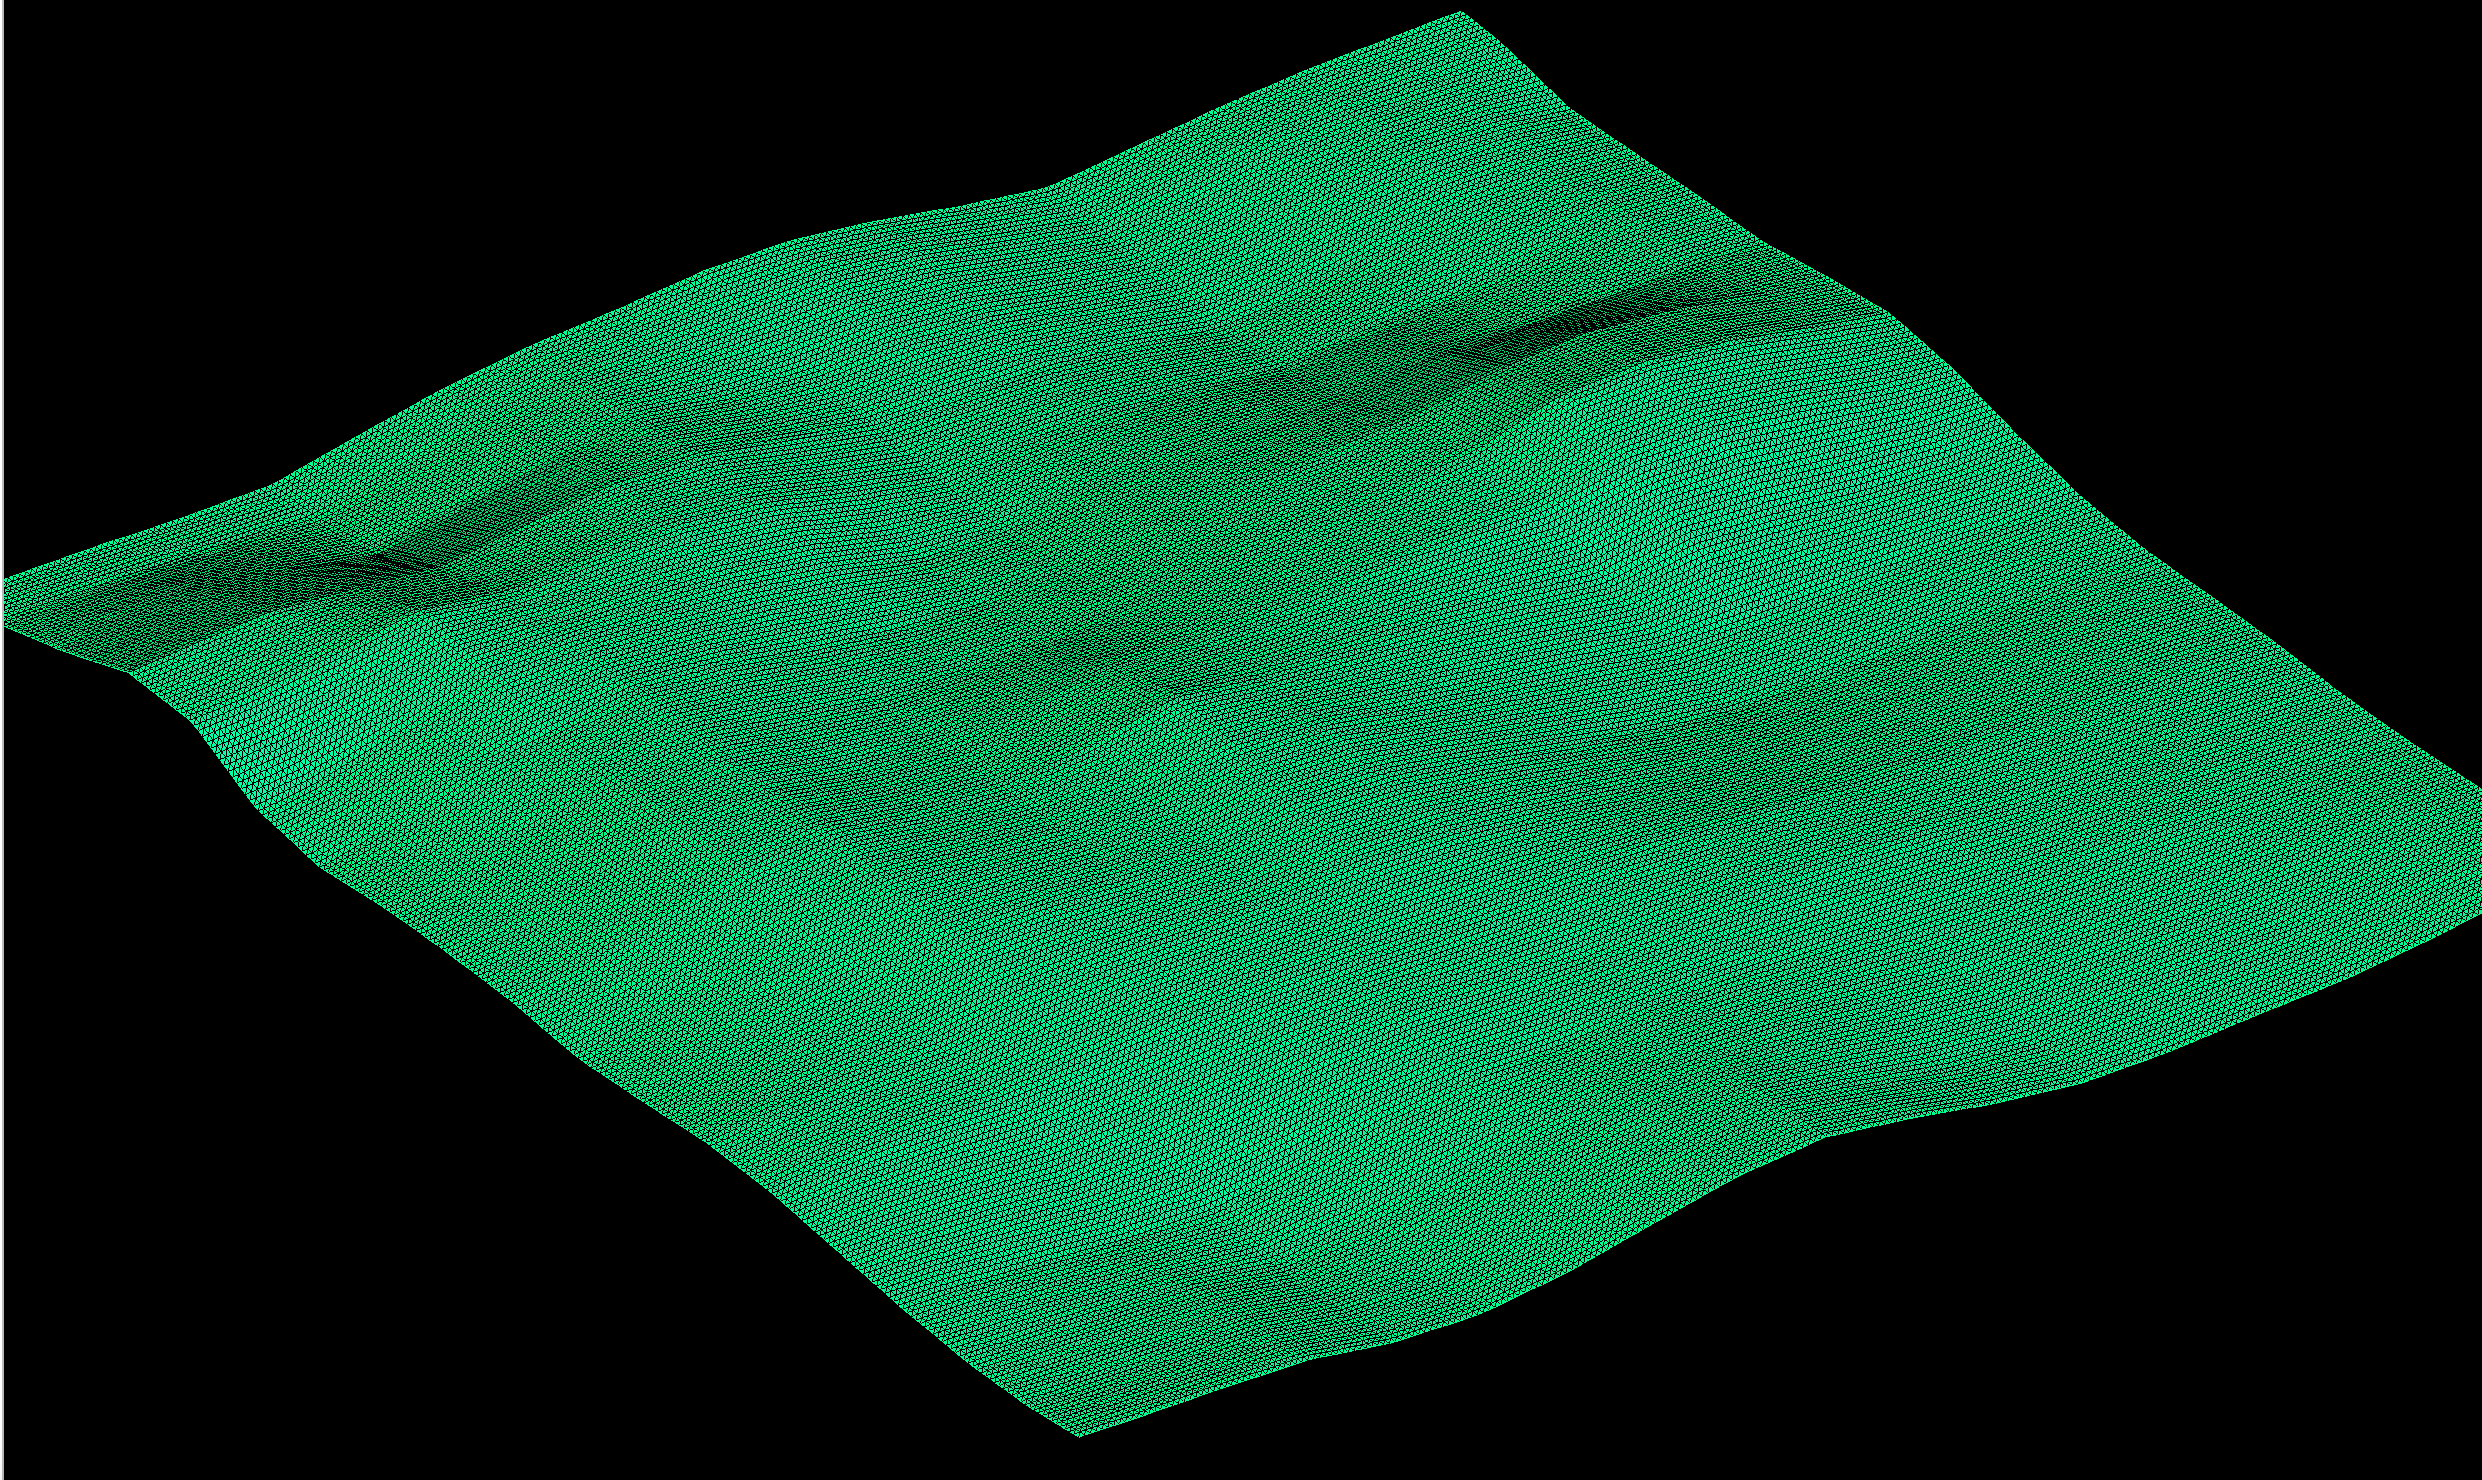
\includegraphics[width=0.8\textwidth]{images/generated-grenoble-16.png}
      \captionsetup{font={scriptsize}}
      \caption{3D mesh \textbf{GPS}}
  \end{figure}
\end{frame}

\begin{frame}{Implementation: Contour lines generation}
  \Large
  \textbf{ContourConstraint} class:
  \vspace{1em}
  \begin{itemize}
    \item \textbf{computeAllContoursMeshes} function
    \item \textbf{getMinMaxZ} function
    \item \textbf{\textcolor{red}{computeContourMesh}} function
  \end{itemize}
\end{frame}

\begin{frame}{Implementation: Contour lines generation}
  \Large
    \[
    z(x, y) = \sqrt{r^2 - (x - x_0)^2 - (y - y_0)^2}
    \]
  \begin{figure}[H]
      \centering
      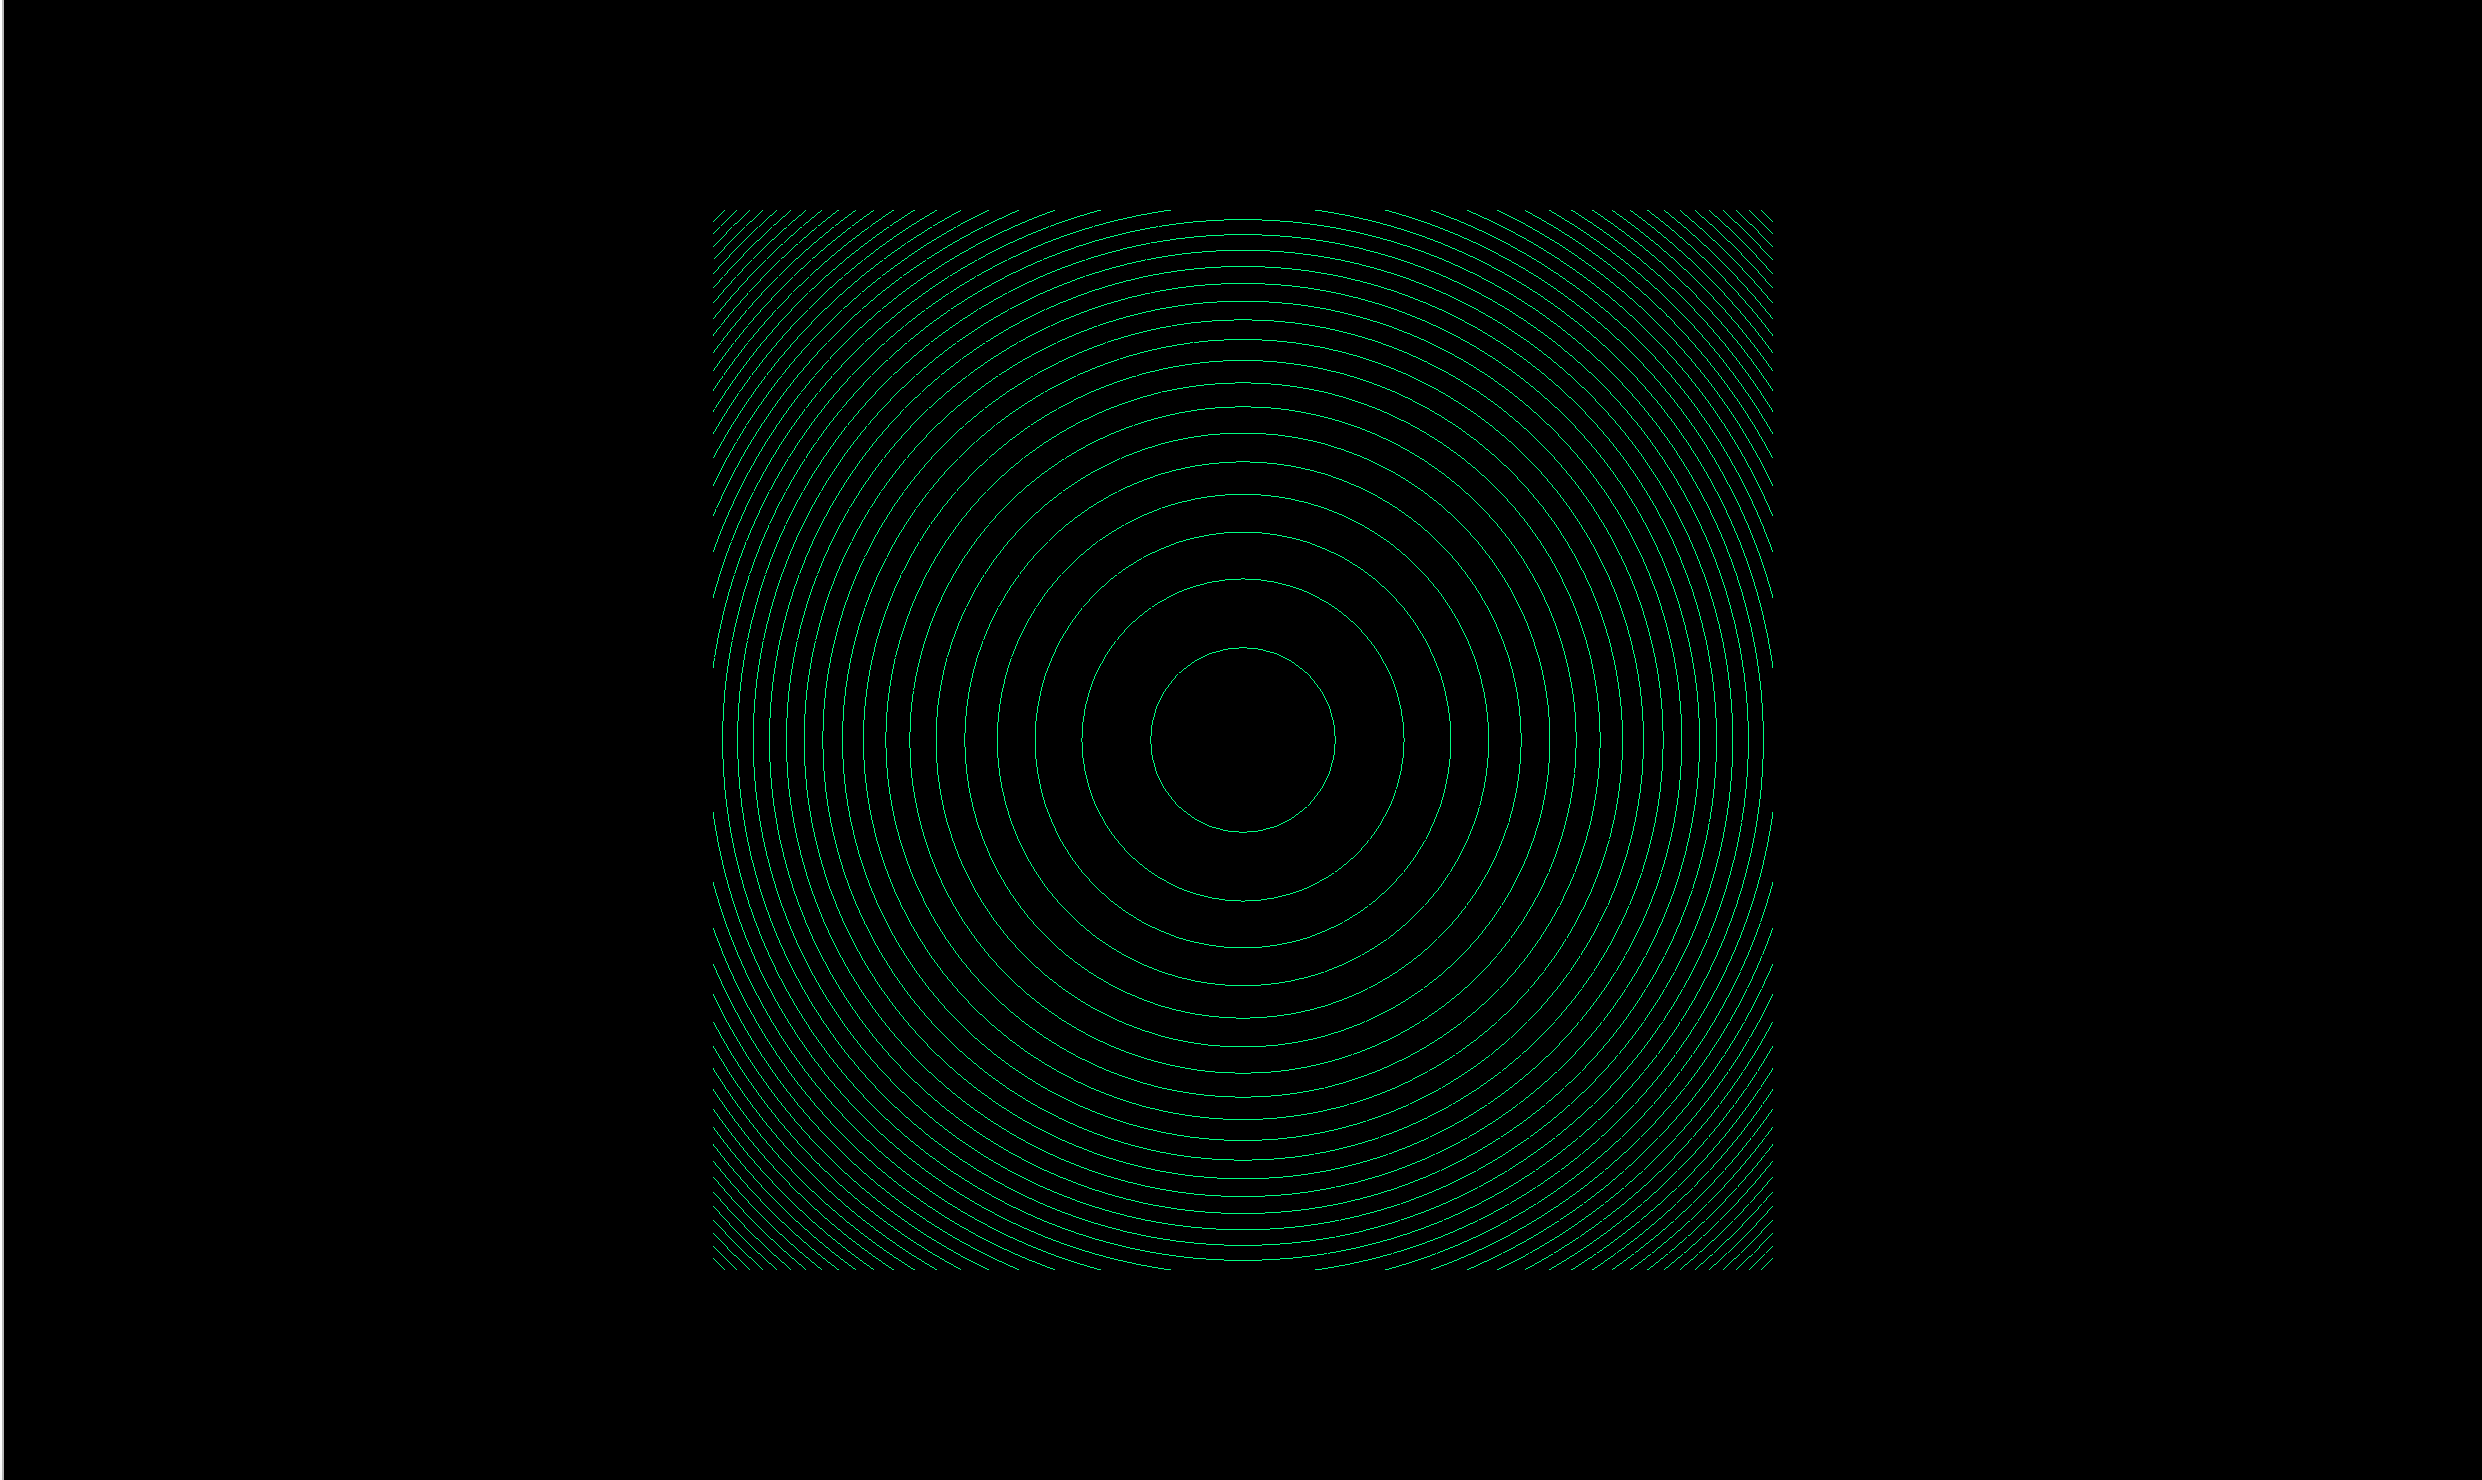
\includegraphics[width=0.8\textwidth]{images/contour-lambda-1-edges.png}
      \captionsetup{font={scriptsize}}
      \caption{3D mesh \textbf{contour lines} 1}
  \end{figure}
\end{frame}

\begin{frame}{Implementation: Contour lines generation}
  \Large
    \[
    z(x, y) = sin(x) + cos(y)
    \]
  \begin{figure}[H]
      \centering
      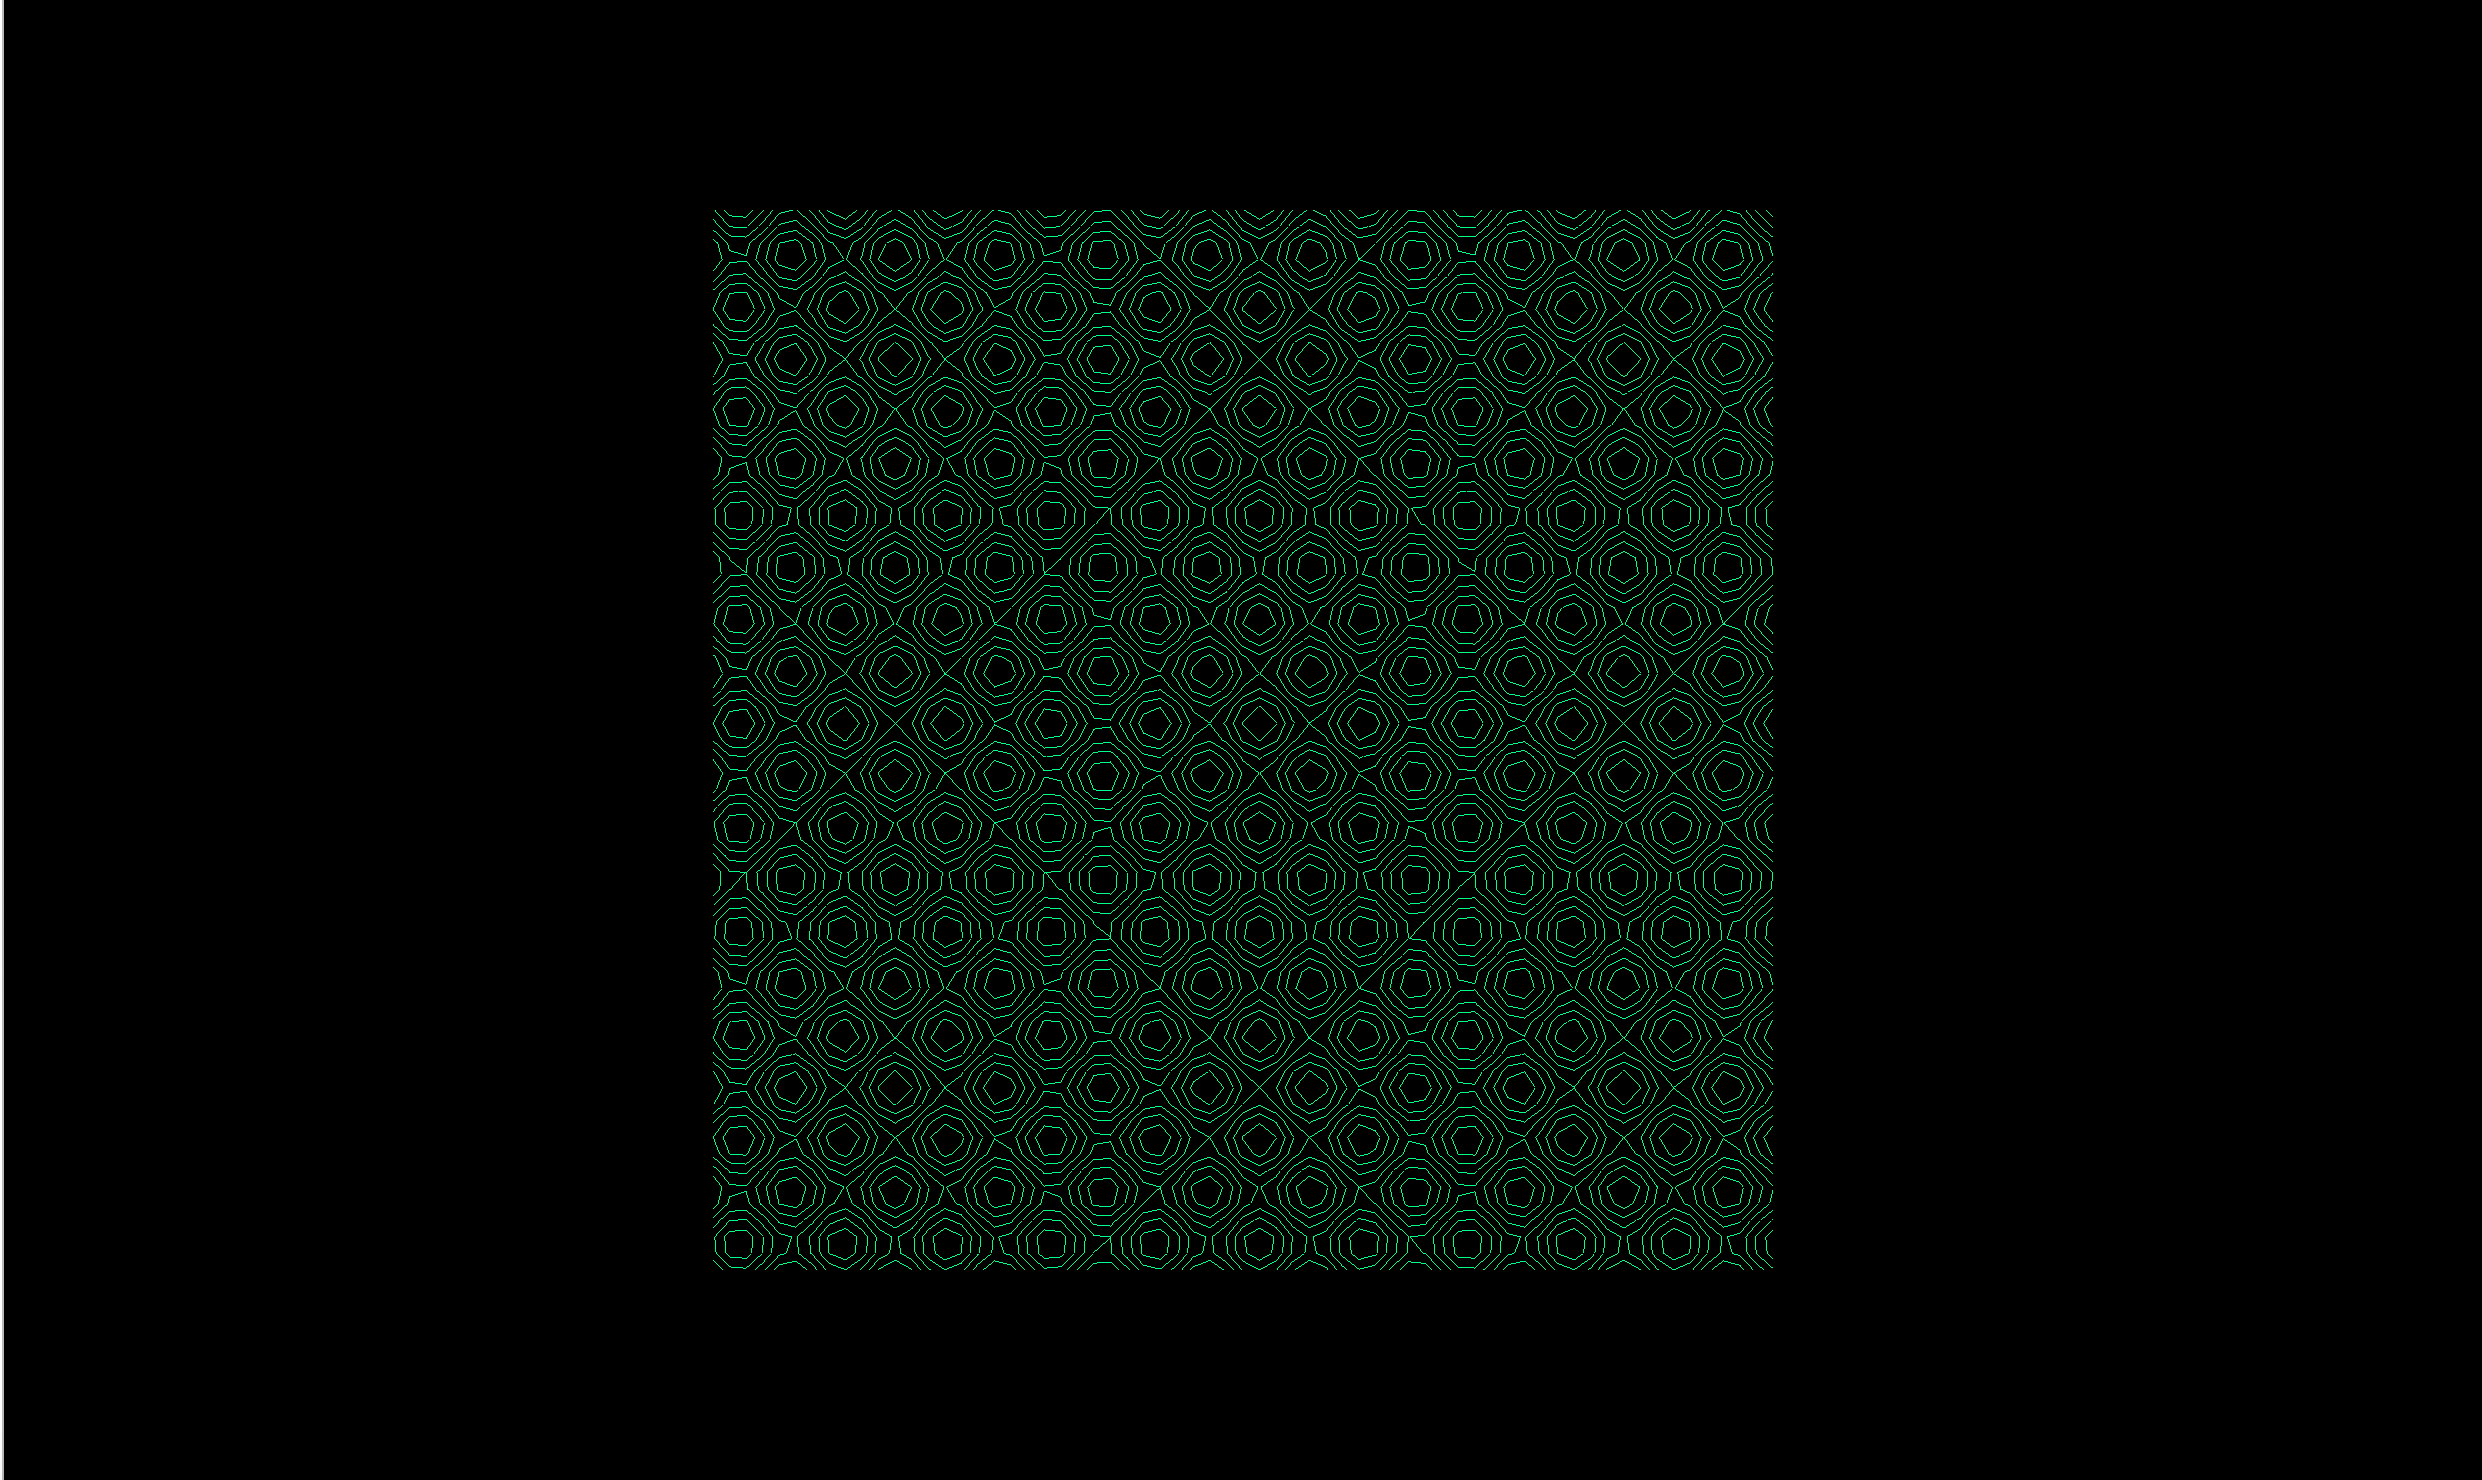
\includegraphics[width=0.8\textwidth]{images/contour-lambda-2-edges.png}
      \captionsetup{font={scriptsize}}
      \caption{3D mesh \textbf{contour lines} 2}
  \end{figure}
\end{frame}

\begin{frame}{Implementation: Contour lines generation}
  \centering
  \Large
  $(x, y) = (33809, 23527)$ at zoom level $16$
  \begin{figure}[H]
      \centering
      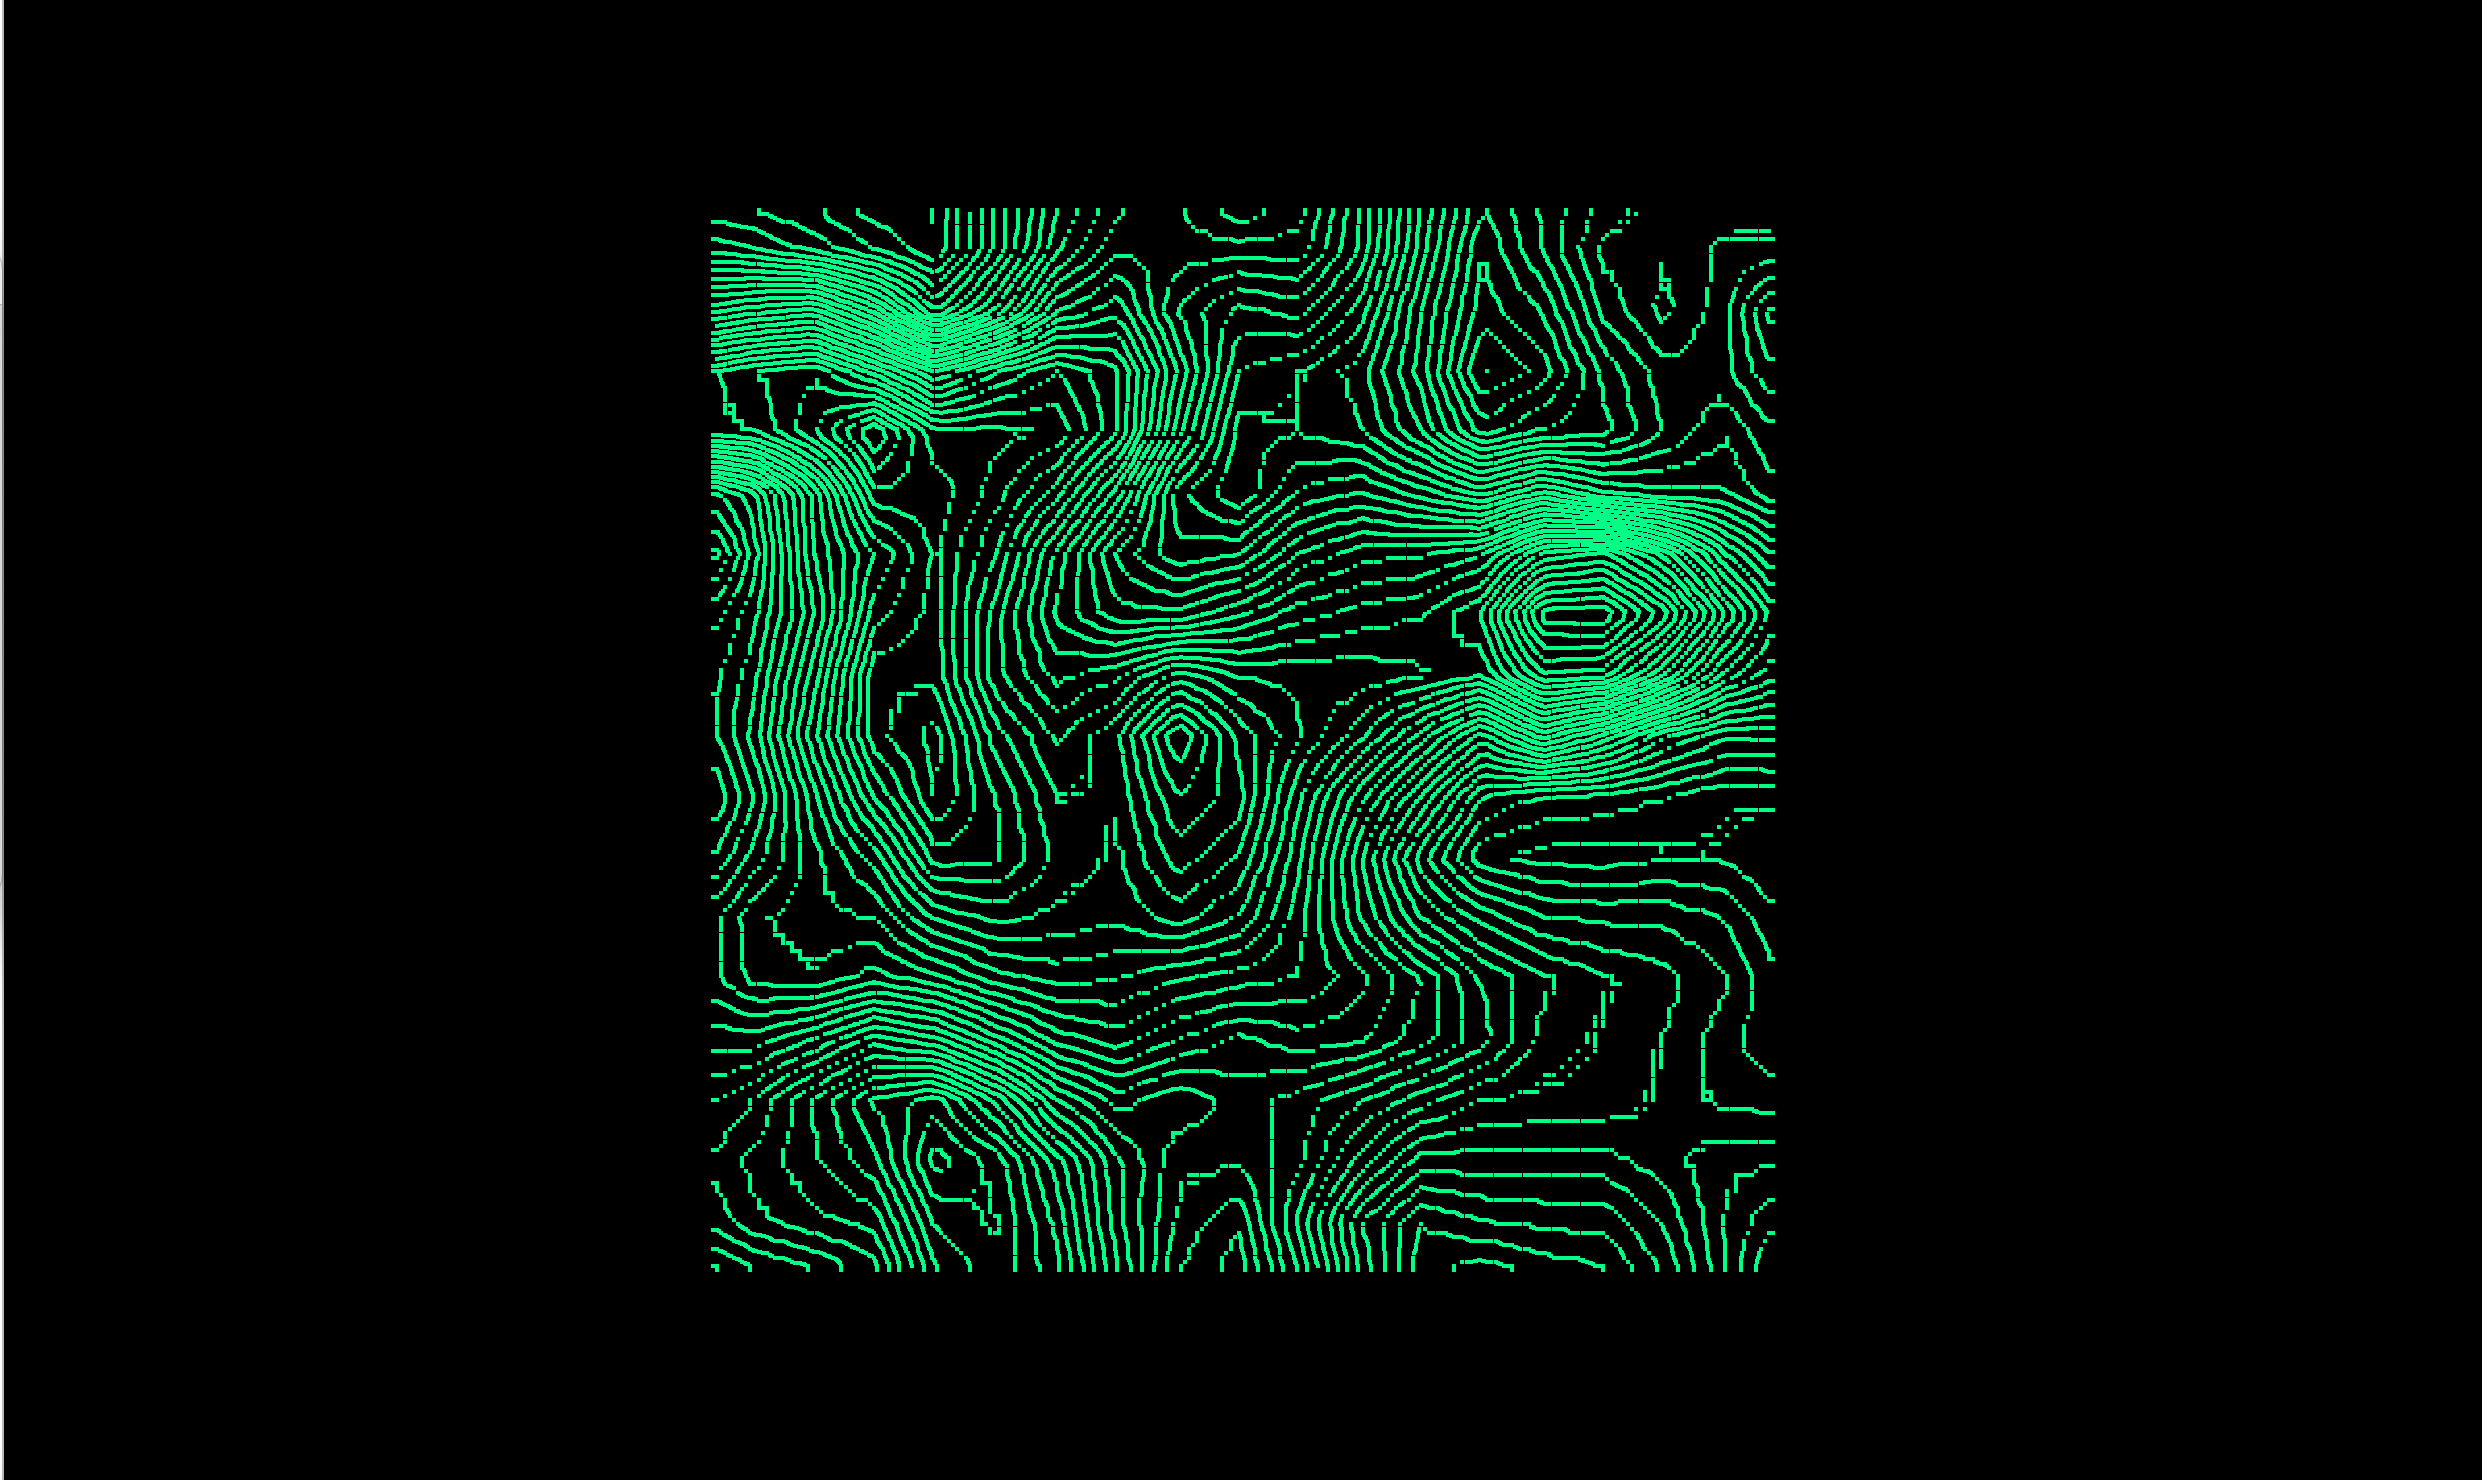
\includegraphics[width=0.8\textwidth]{images/contour-strasbourg-16-1.png}
      \captionsetup{font={scriptsize}}
      \caption{3D mesh \textbf{contour lines GPS}}
  \end{figure}
\end{frame}

\begin{frame}{Implementation: Re-triangulation}
  \Large
  \textbf{\textcolor{red}{triangulateAssembledMesh}} function:
  \vspace{1em}
  \begin{itemize}
    \item \textbf{Inserting constraints} into \textbf{Constrained\_Delaunay\_triangulation\_2}
    \item \textbf{CGAL::make\_conforming\_Delaunay\_2}
    \item \textbf{Generating} the \textbf{final mesh}
  \end{itemize}
\end{frame}

\begin{frame}{Results}
  \Large
  \[
  z(x, y) = \sqrt{r^2 - (x - x_0)^2 - (y - y_0)^2}
  \]
  \begin{figure}[H]
    \centering
    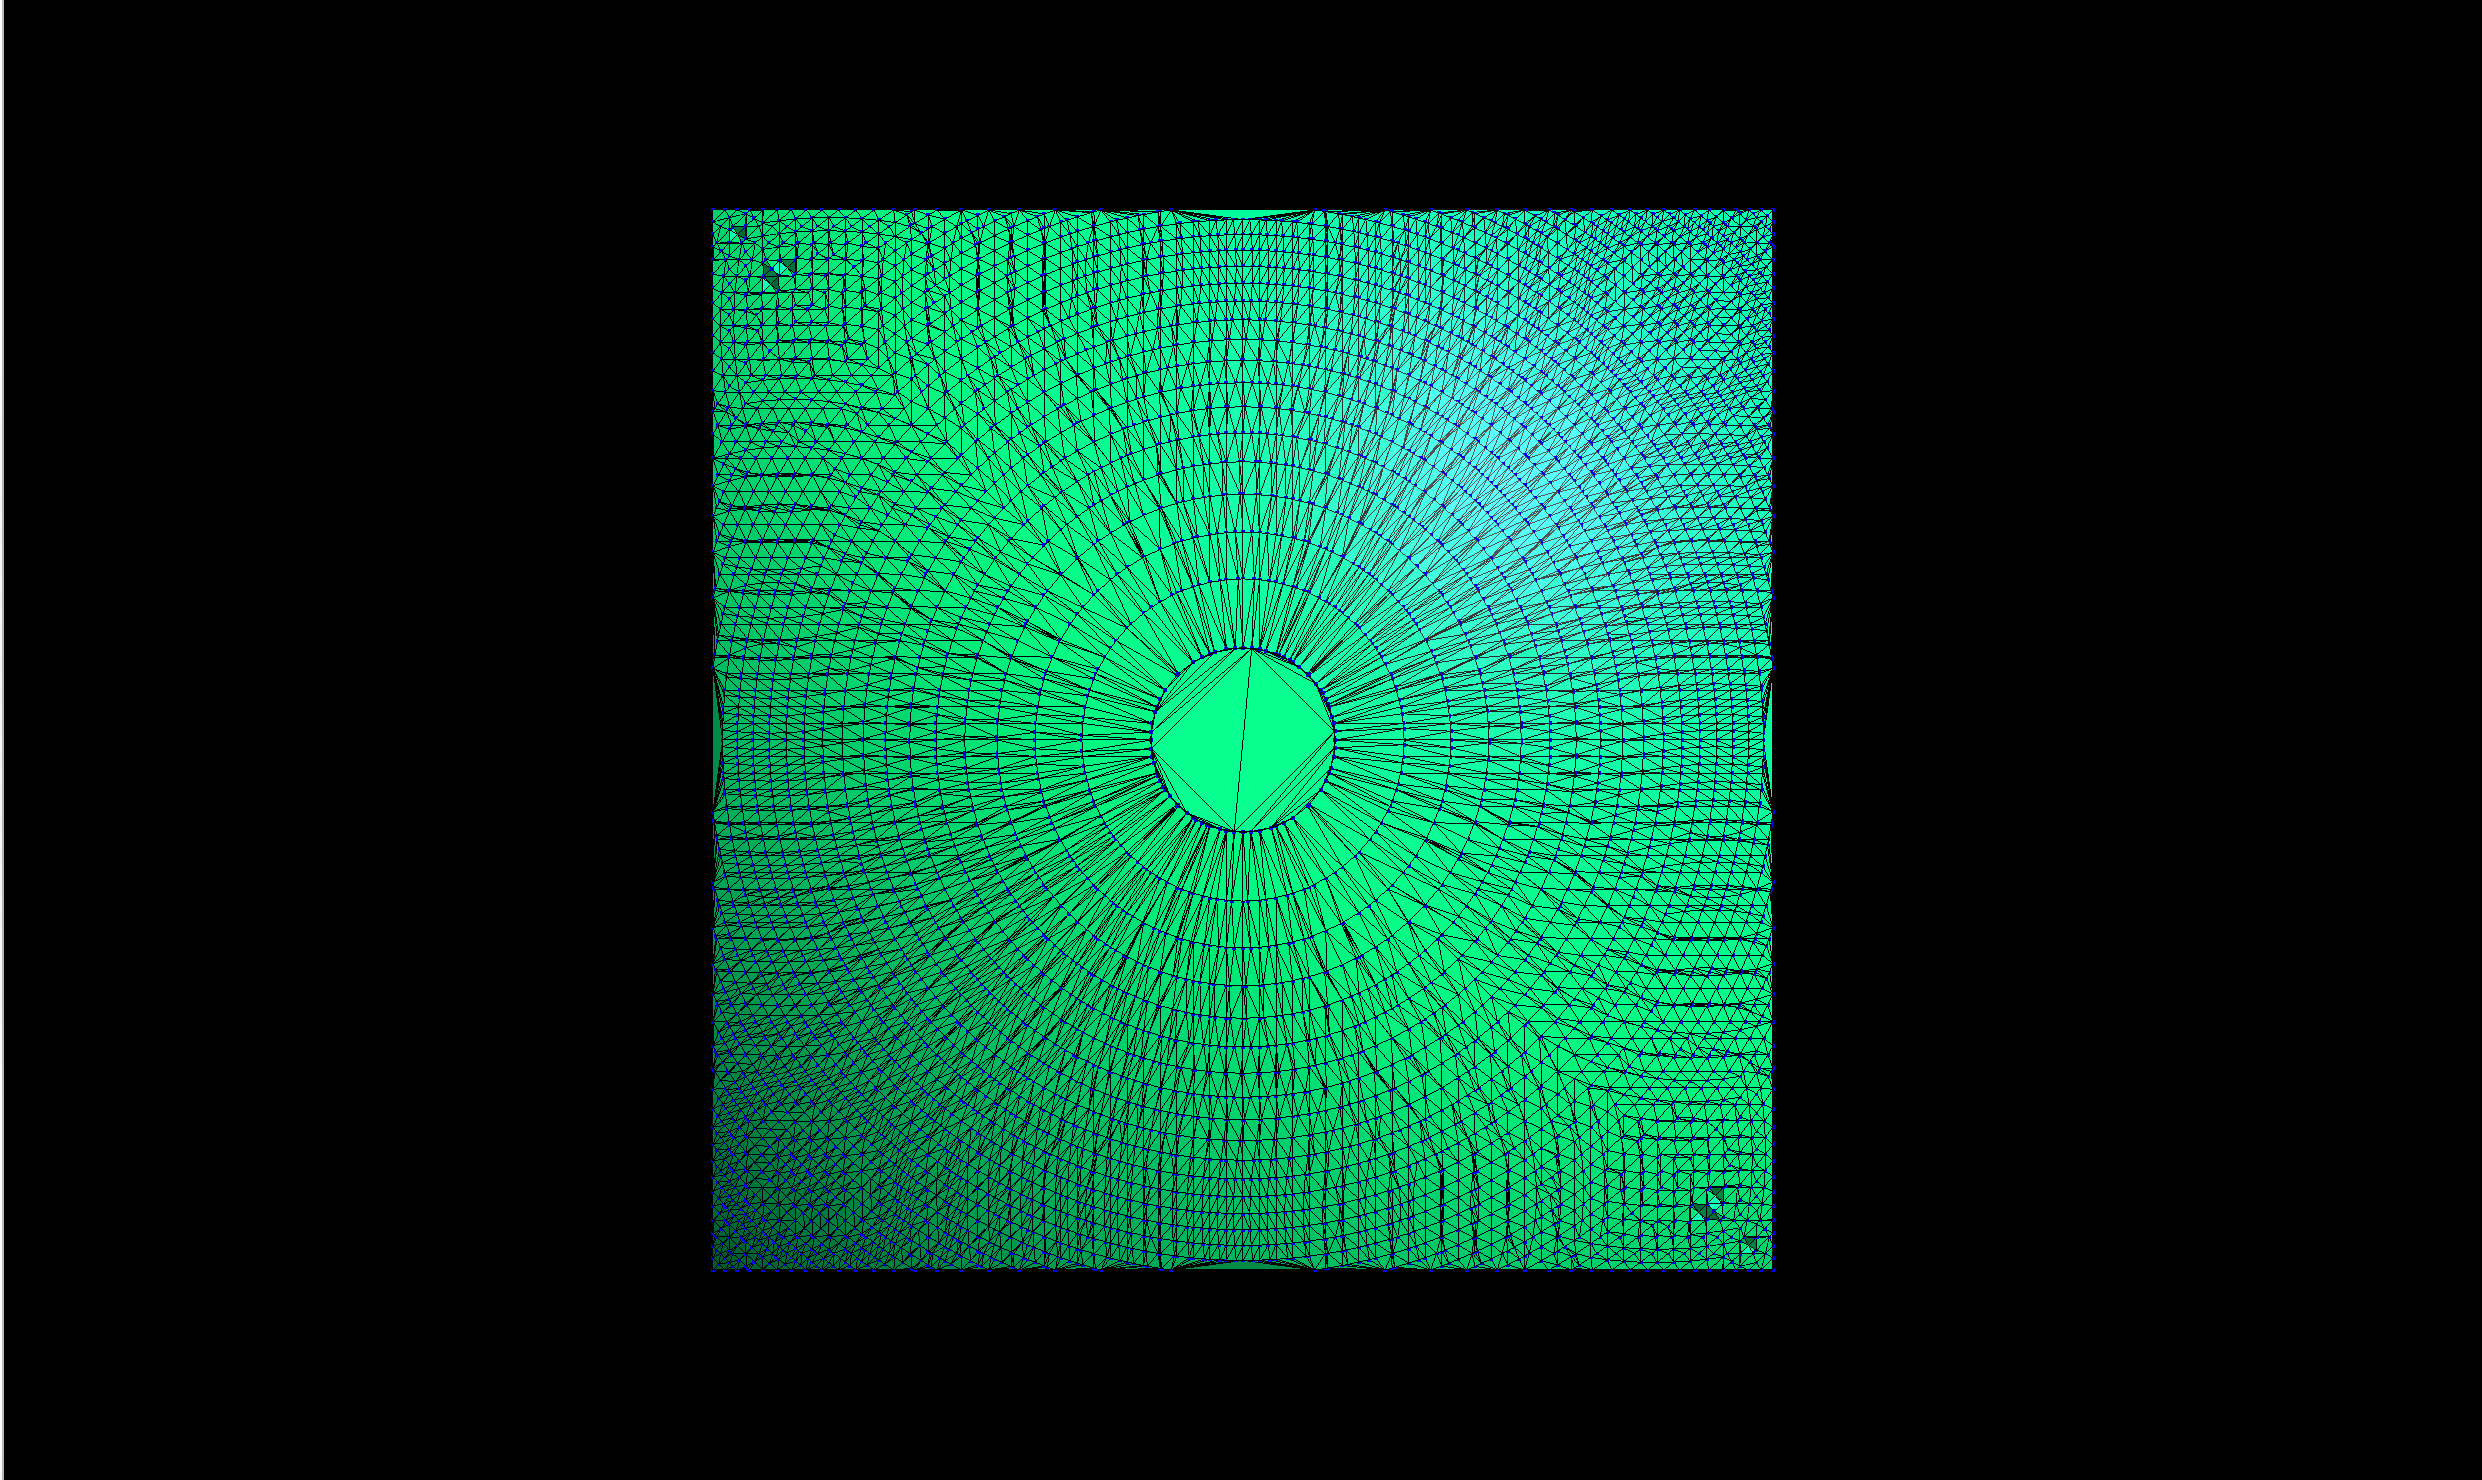
\includegraphics[width=0.8\textwidth]{images/constrained-lambda-1.png}
    \captionsetup{font={scriptsize}}
    \caption{3D mesh after re-triangulation (lambda function 1)}
\end{figure}
\end{frame}

\begin{frame}{Results}
  \begin{figure}[H]
    \centering
    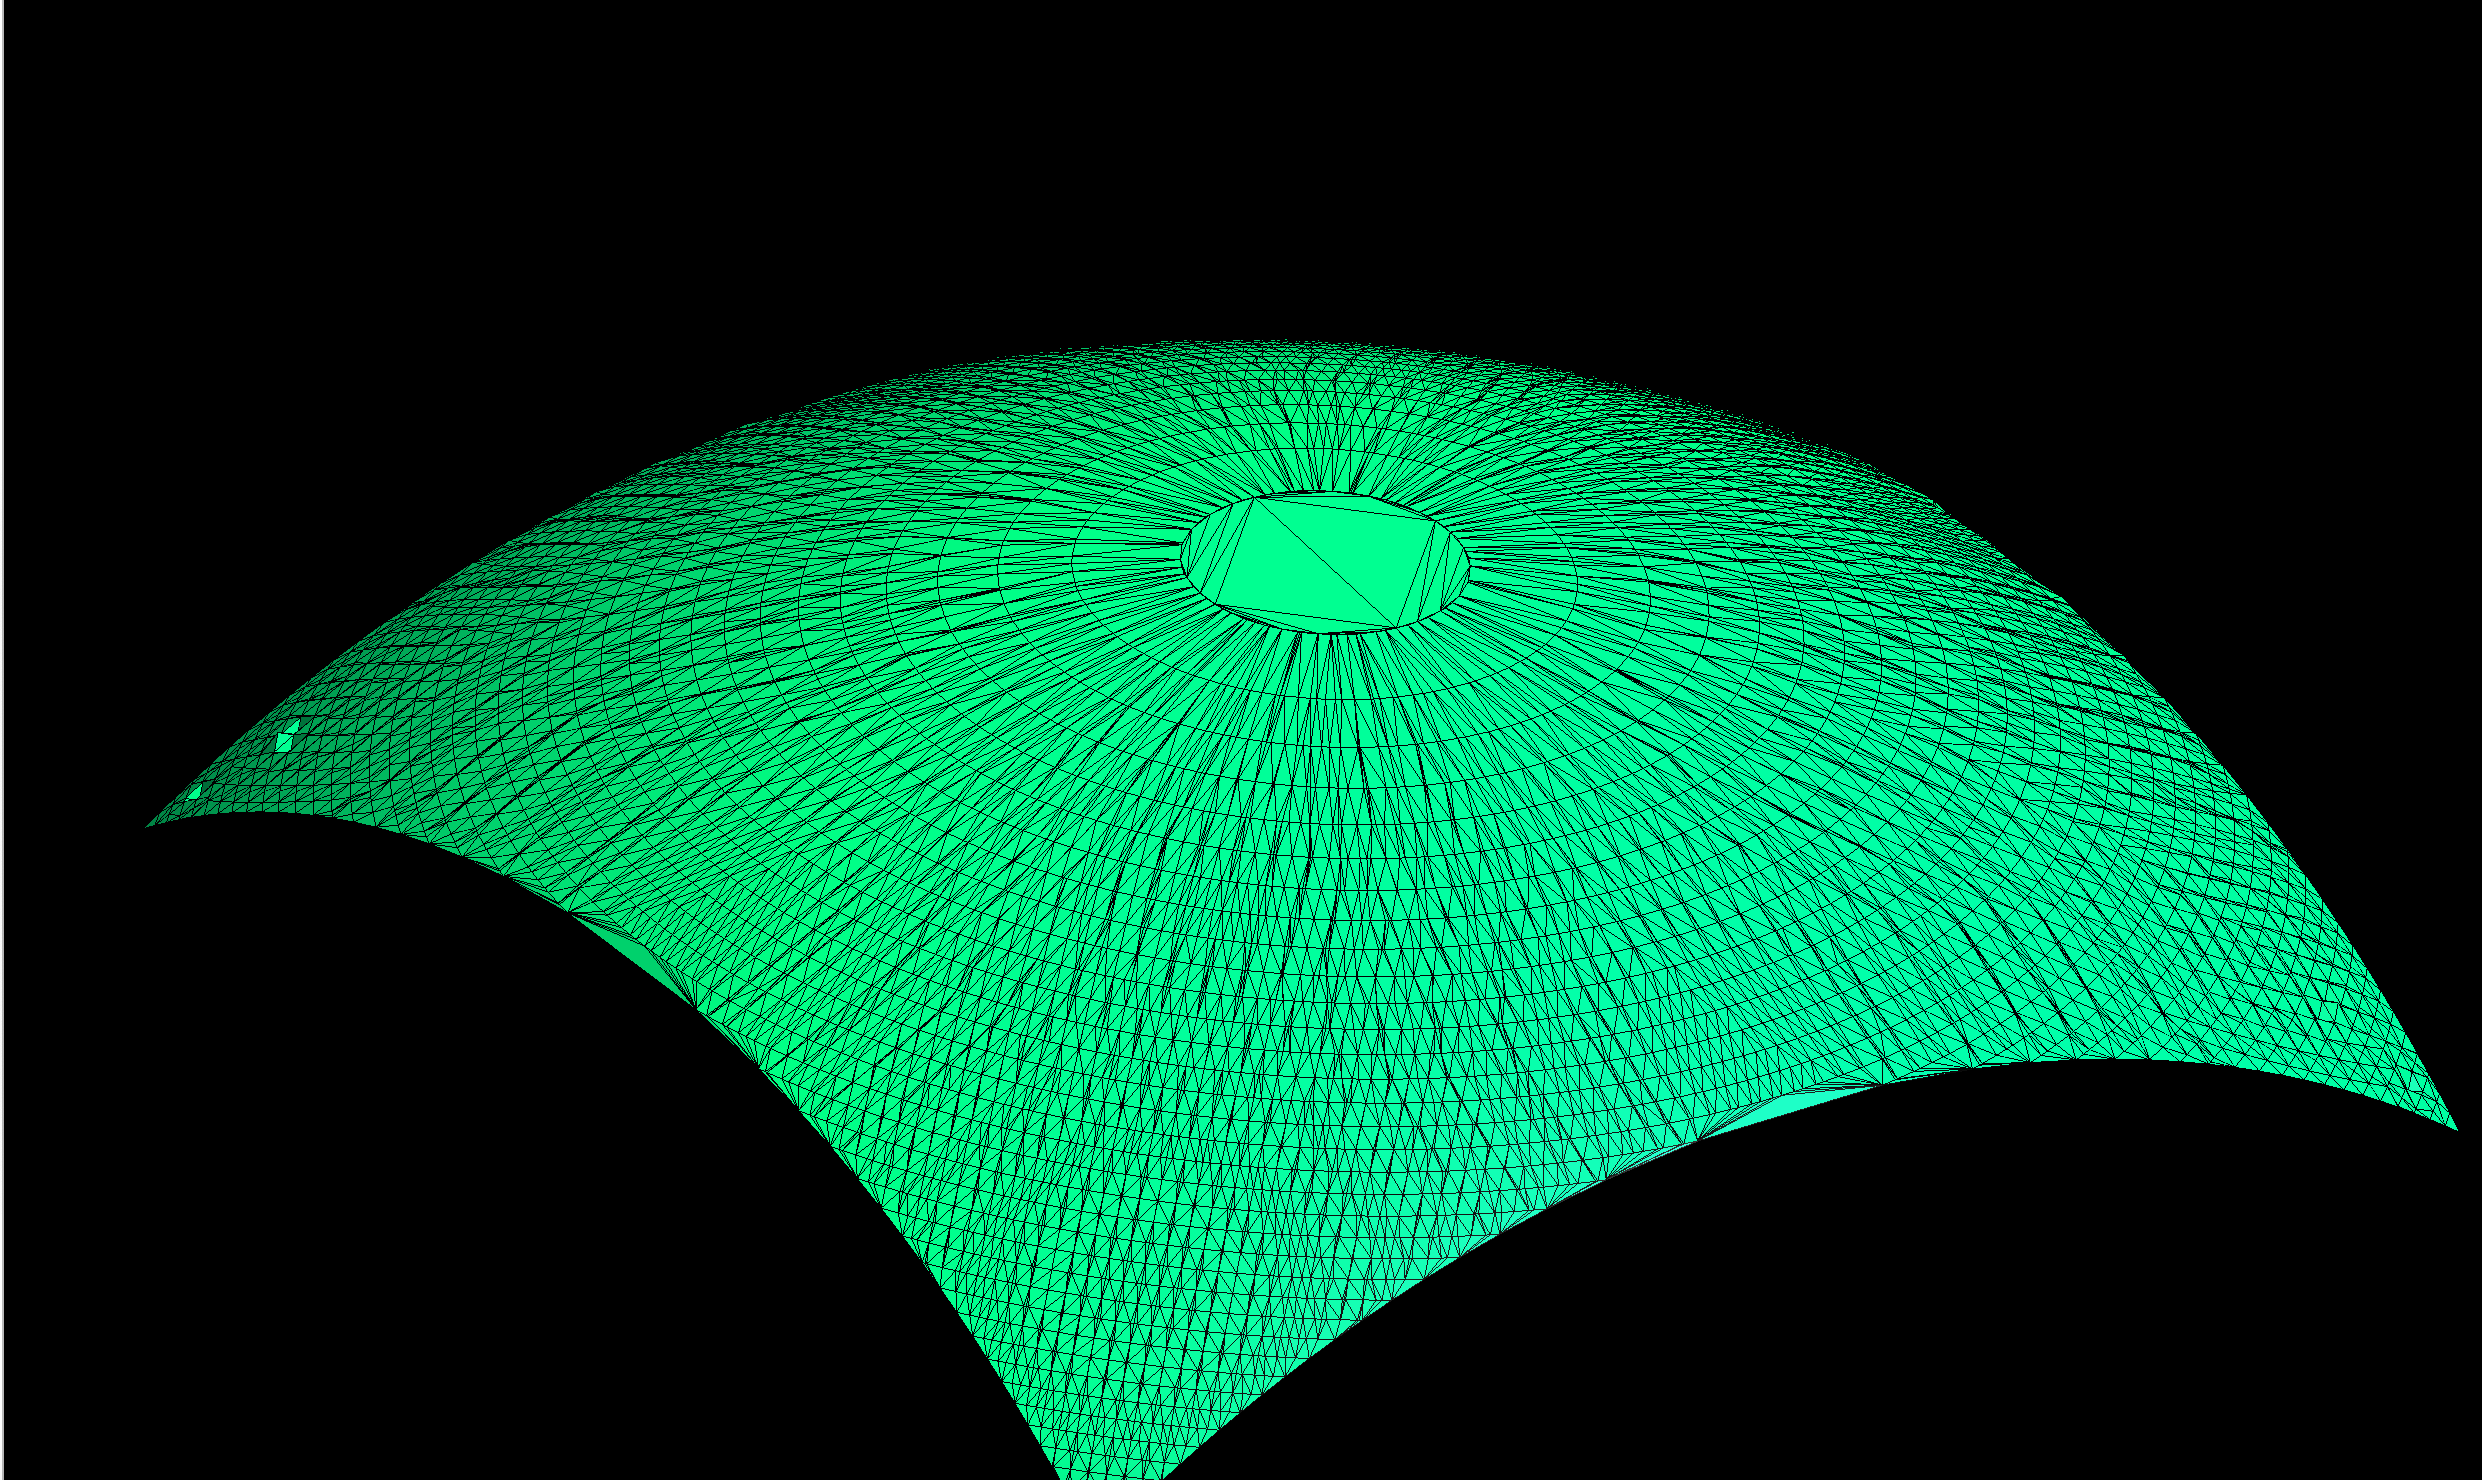
\includegraphics[width=0.8\textwidth]{images/constrained-lambda-1-side.png}
    \captionsetup{font={scriptsize}}
    \caption{3D mesh after re-triangulation (lambda function 1) side view}
\end{figure}
\end{frame}

\begin{frame}{Results}
  \Large
  \[
  z(x, y) = sin(x) + cos(y)
  \]
  \begin{figure}[H]
    \centering
    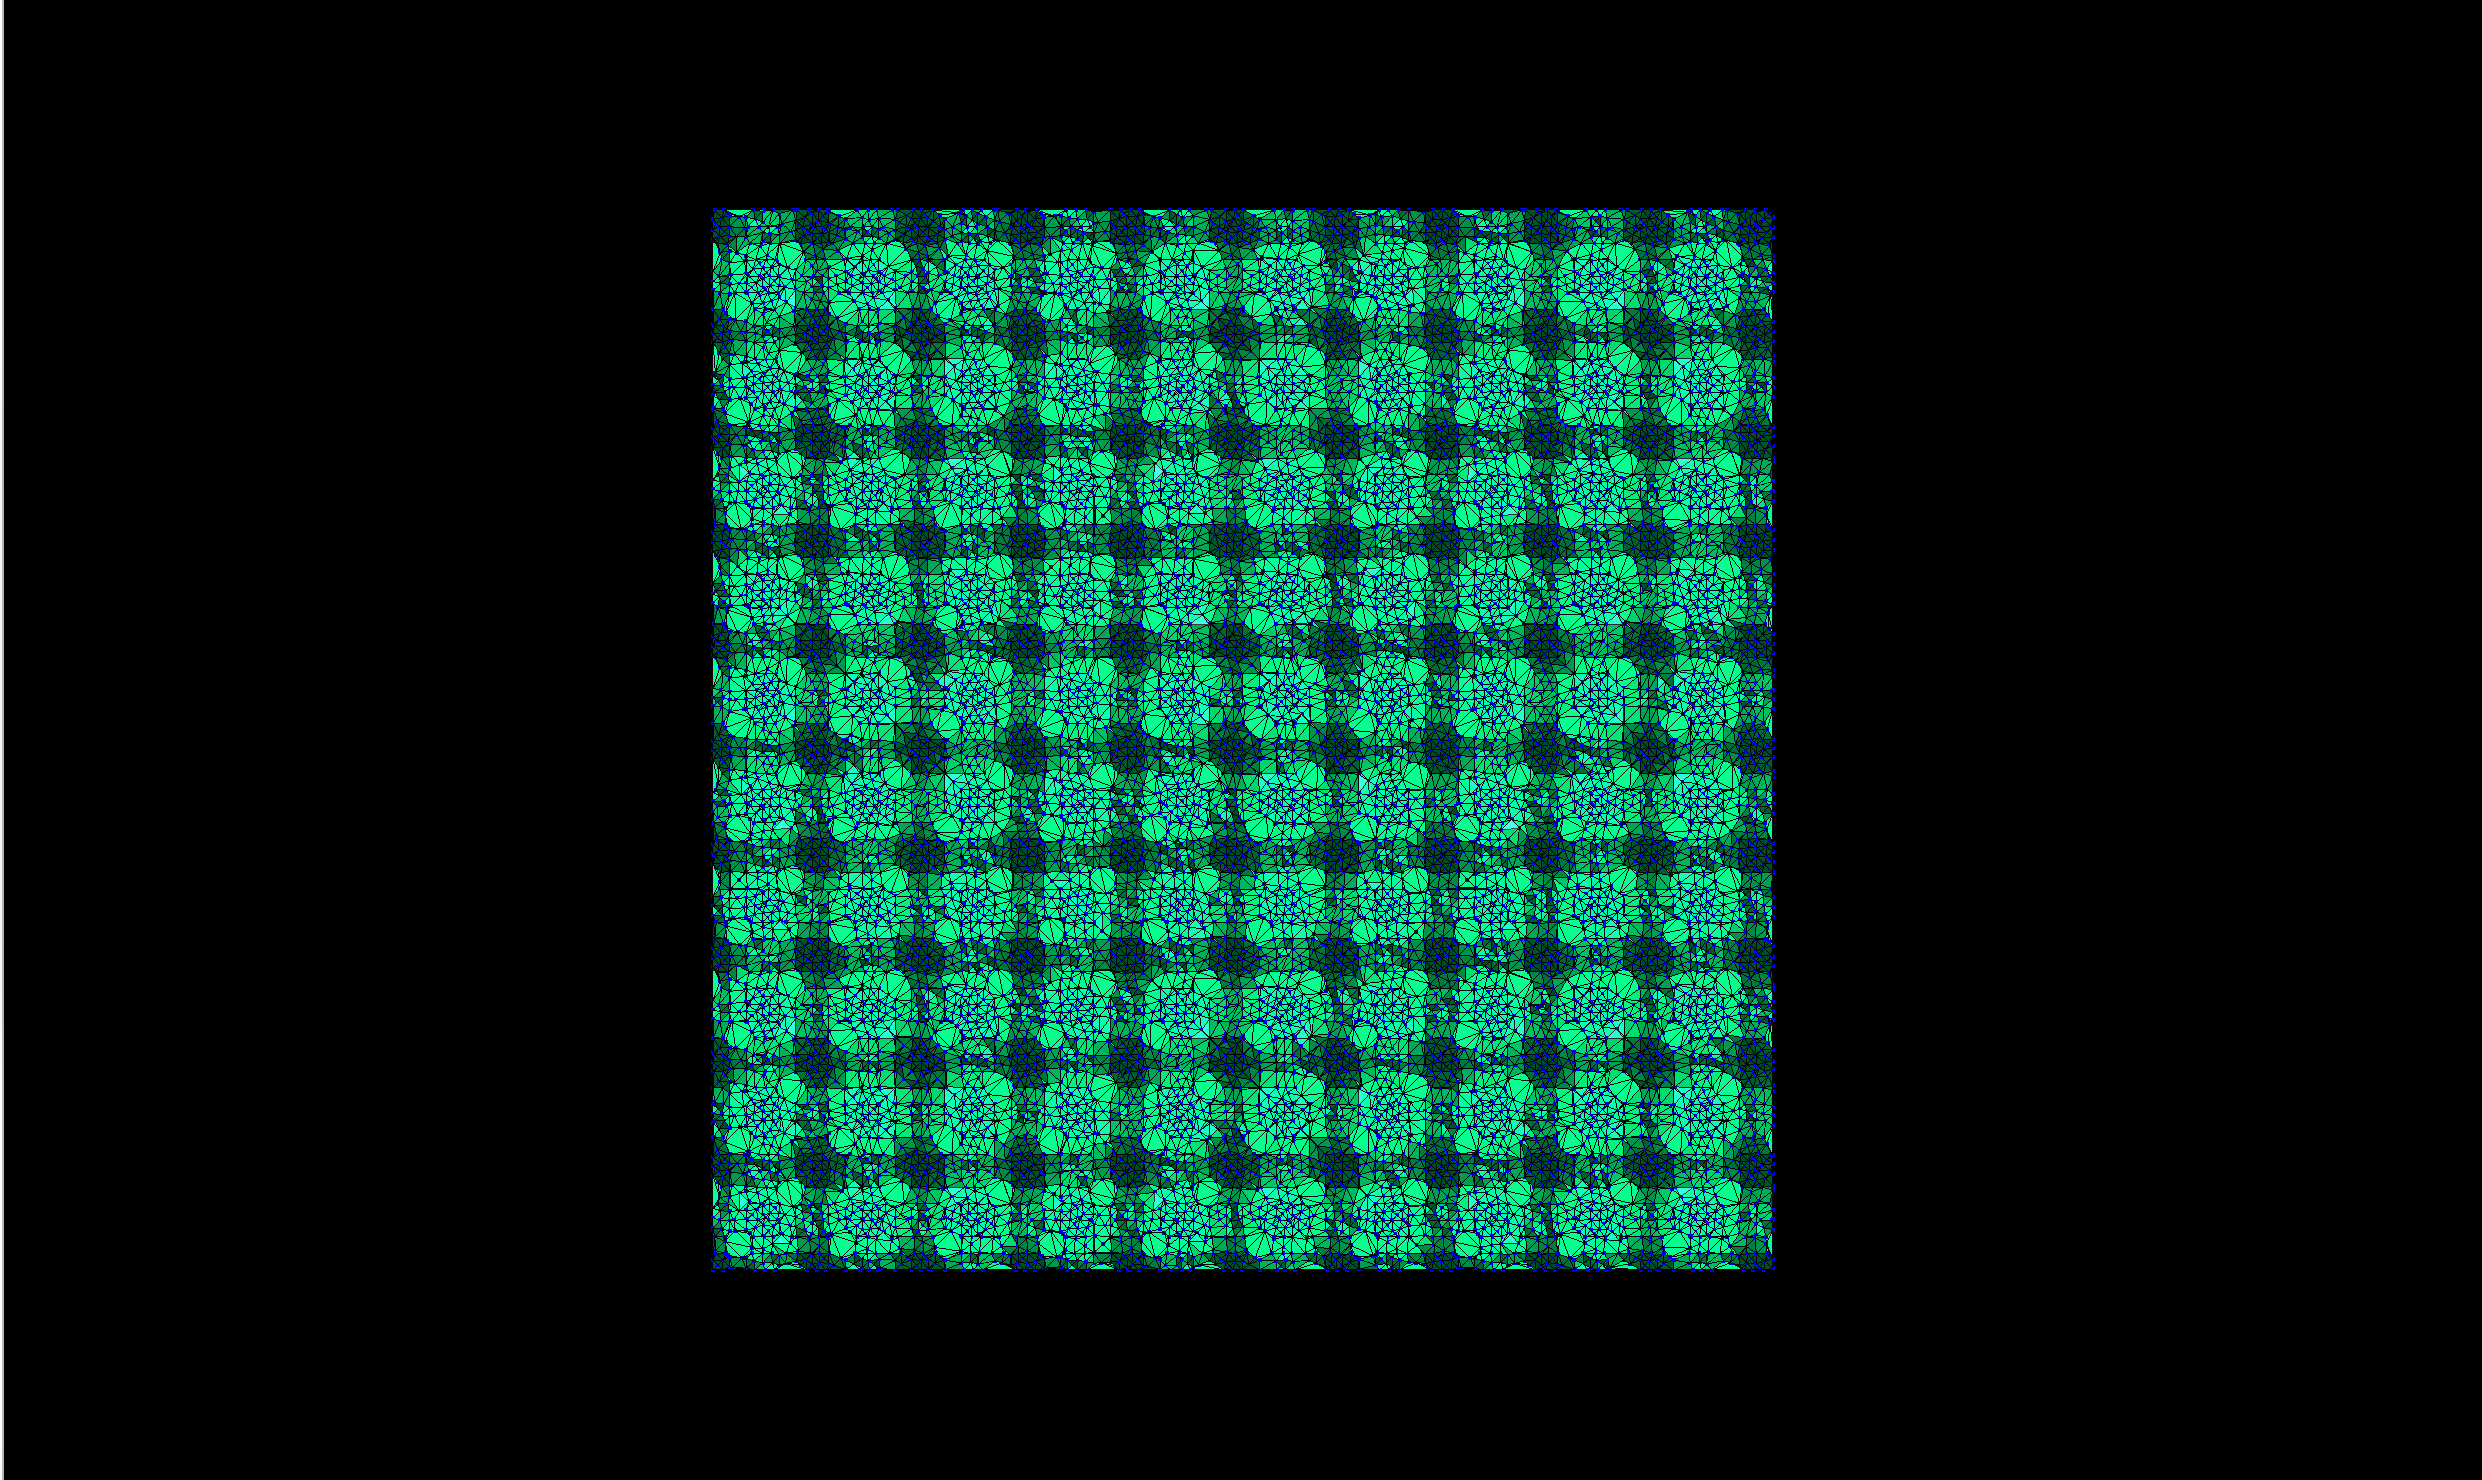
\includegraphics[width=0.8\textwidth]{images/constrained-lambda-2.png}
    \captionsetup{font={scriptsize}}
    \caption{3D mesh after re-triangulation (lambda function 2)}
\end{figure}
\end{frame}

\begin{frame}{Results}
  \begin{figure}[H]
    \centering
    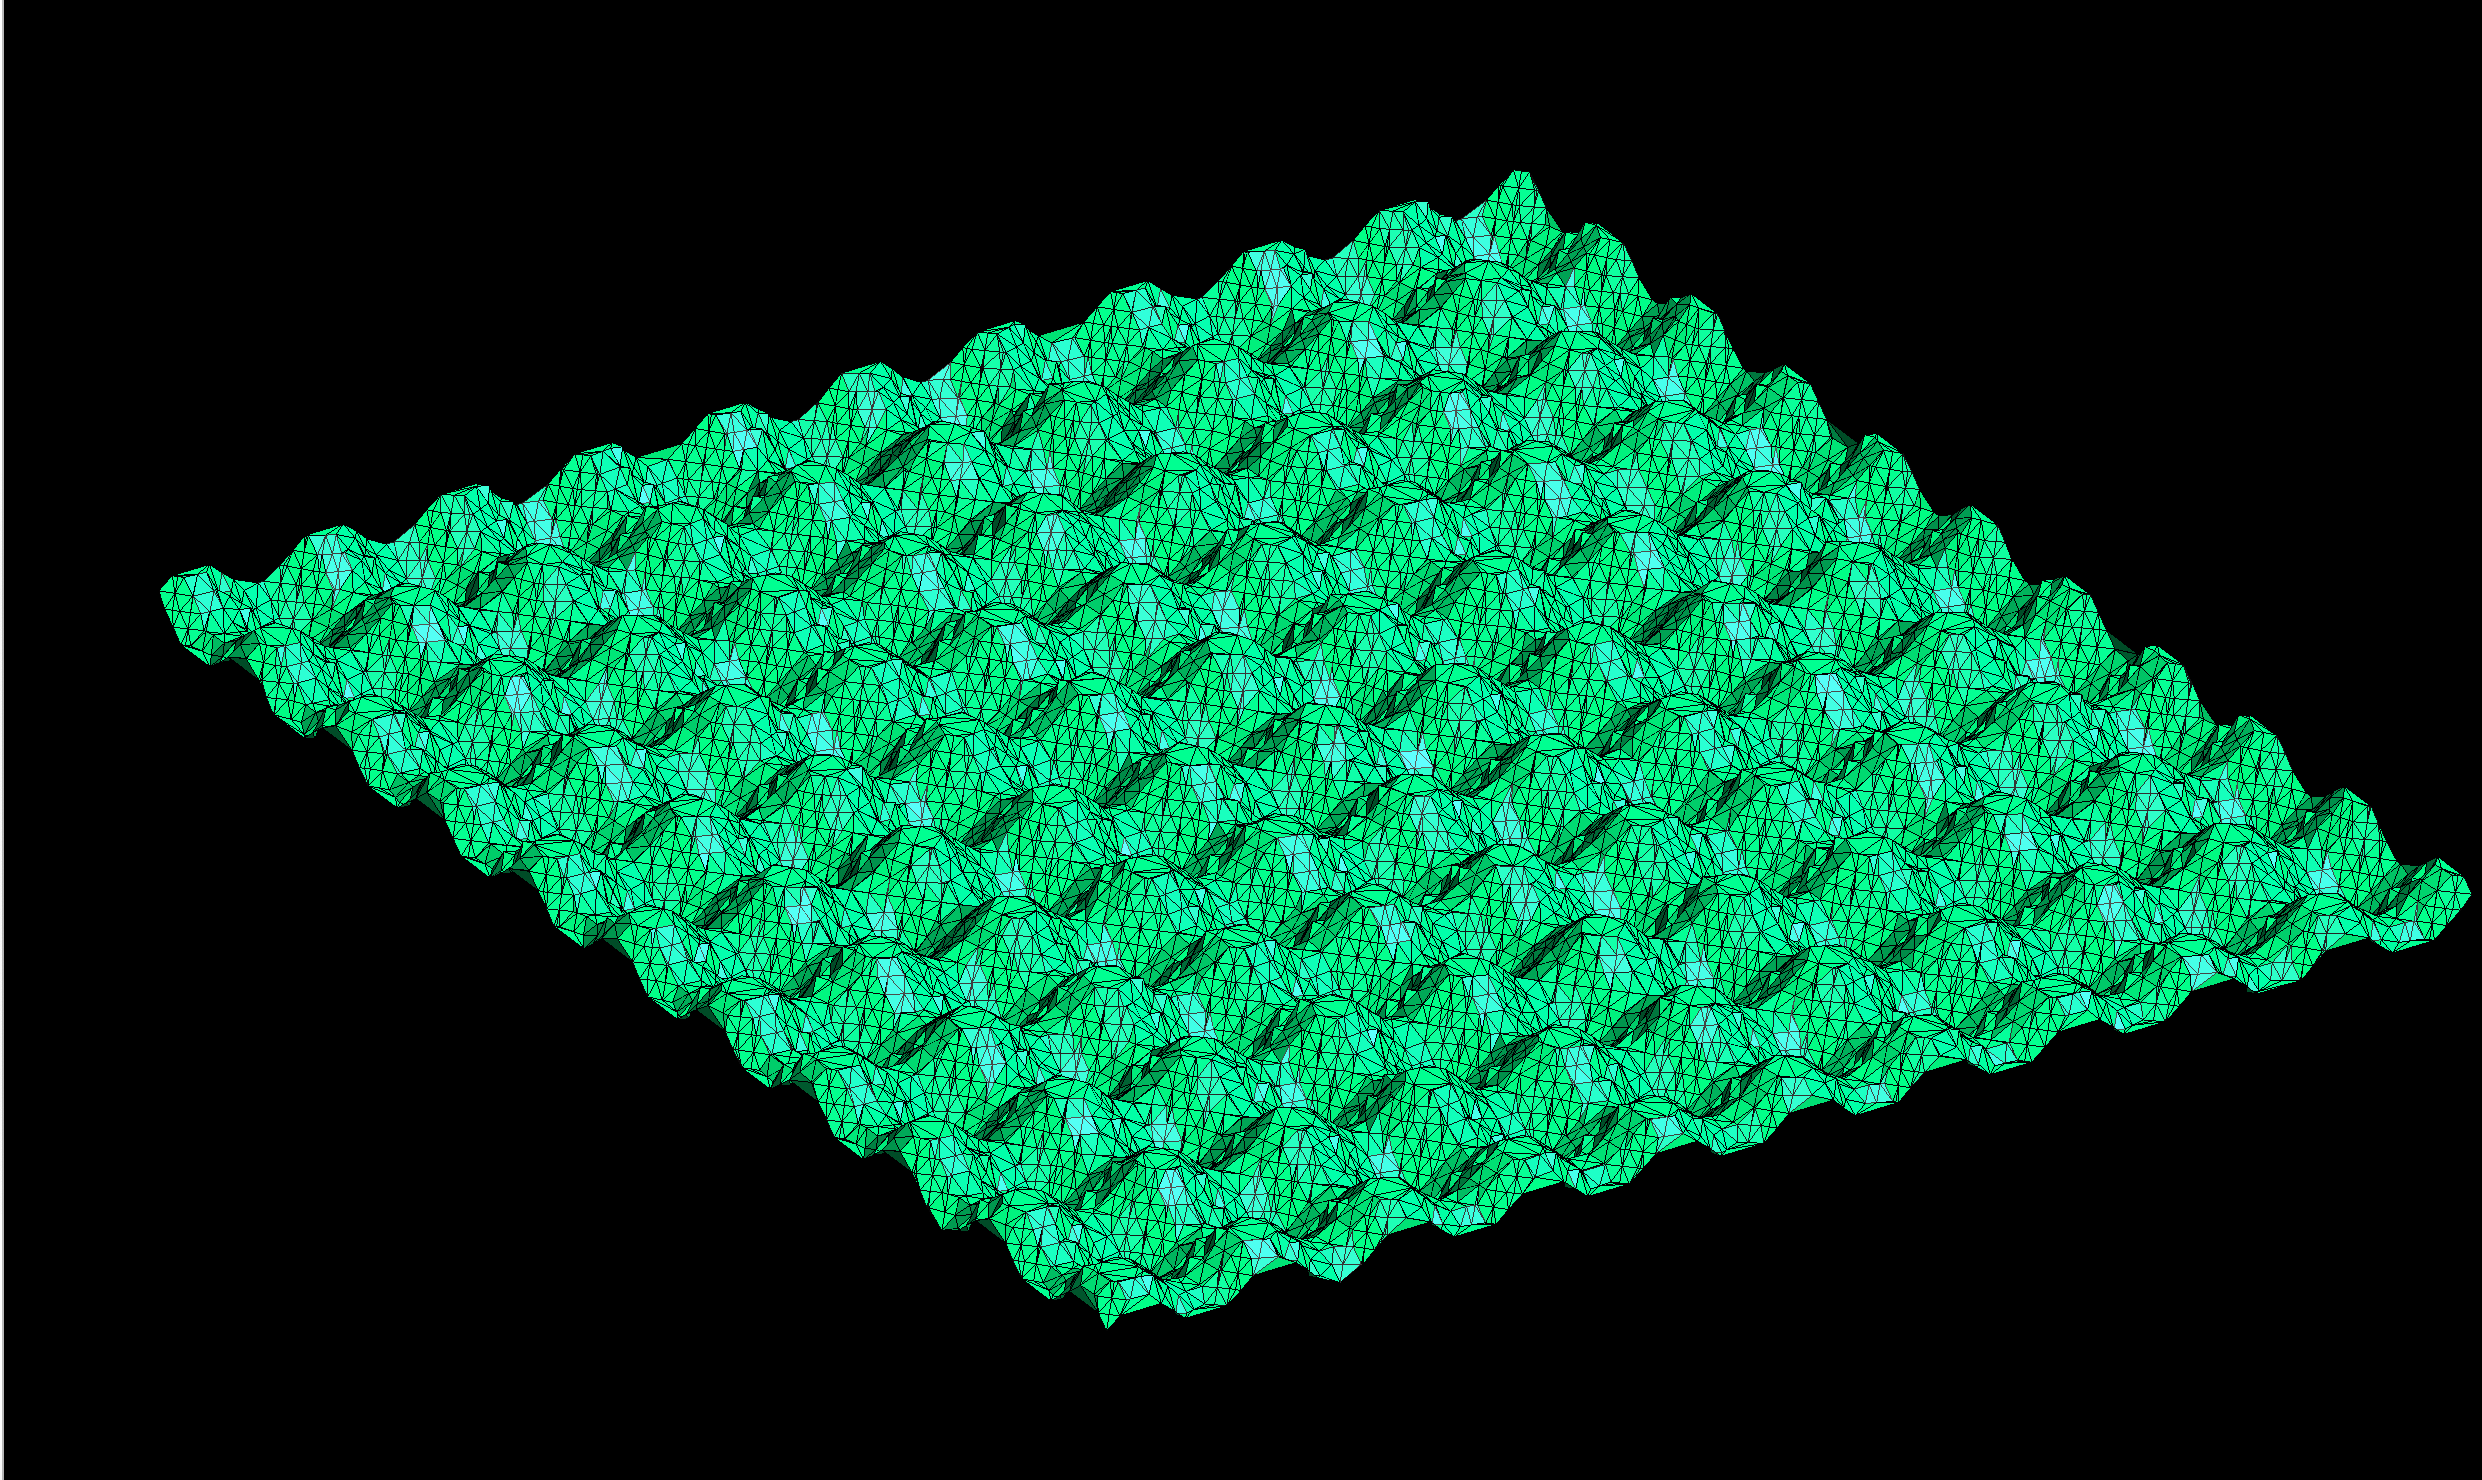
\includegraphics[width=0.8\textwidth]{images/constrained-lambda-2-side.png}
    \captionsetup{font={scriptsize}}
    \caption{3D mesh after re-triangulation (lambda function 2) side view}
\end{figure}
\end{frame}

\begin{frame}{Results}
  \centering
  \Large
  $(x, y) = (33809, 23527)$ at zoom level $16$
  \begin{figure}[H]
    \centering
    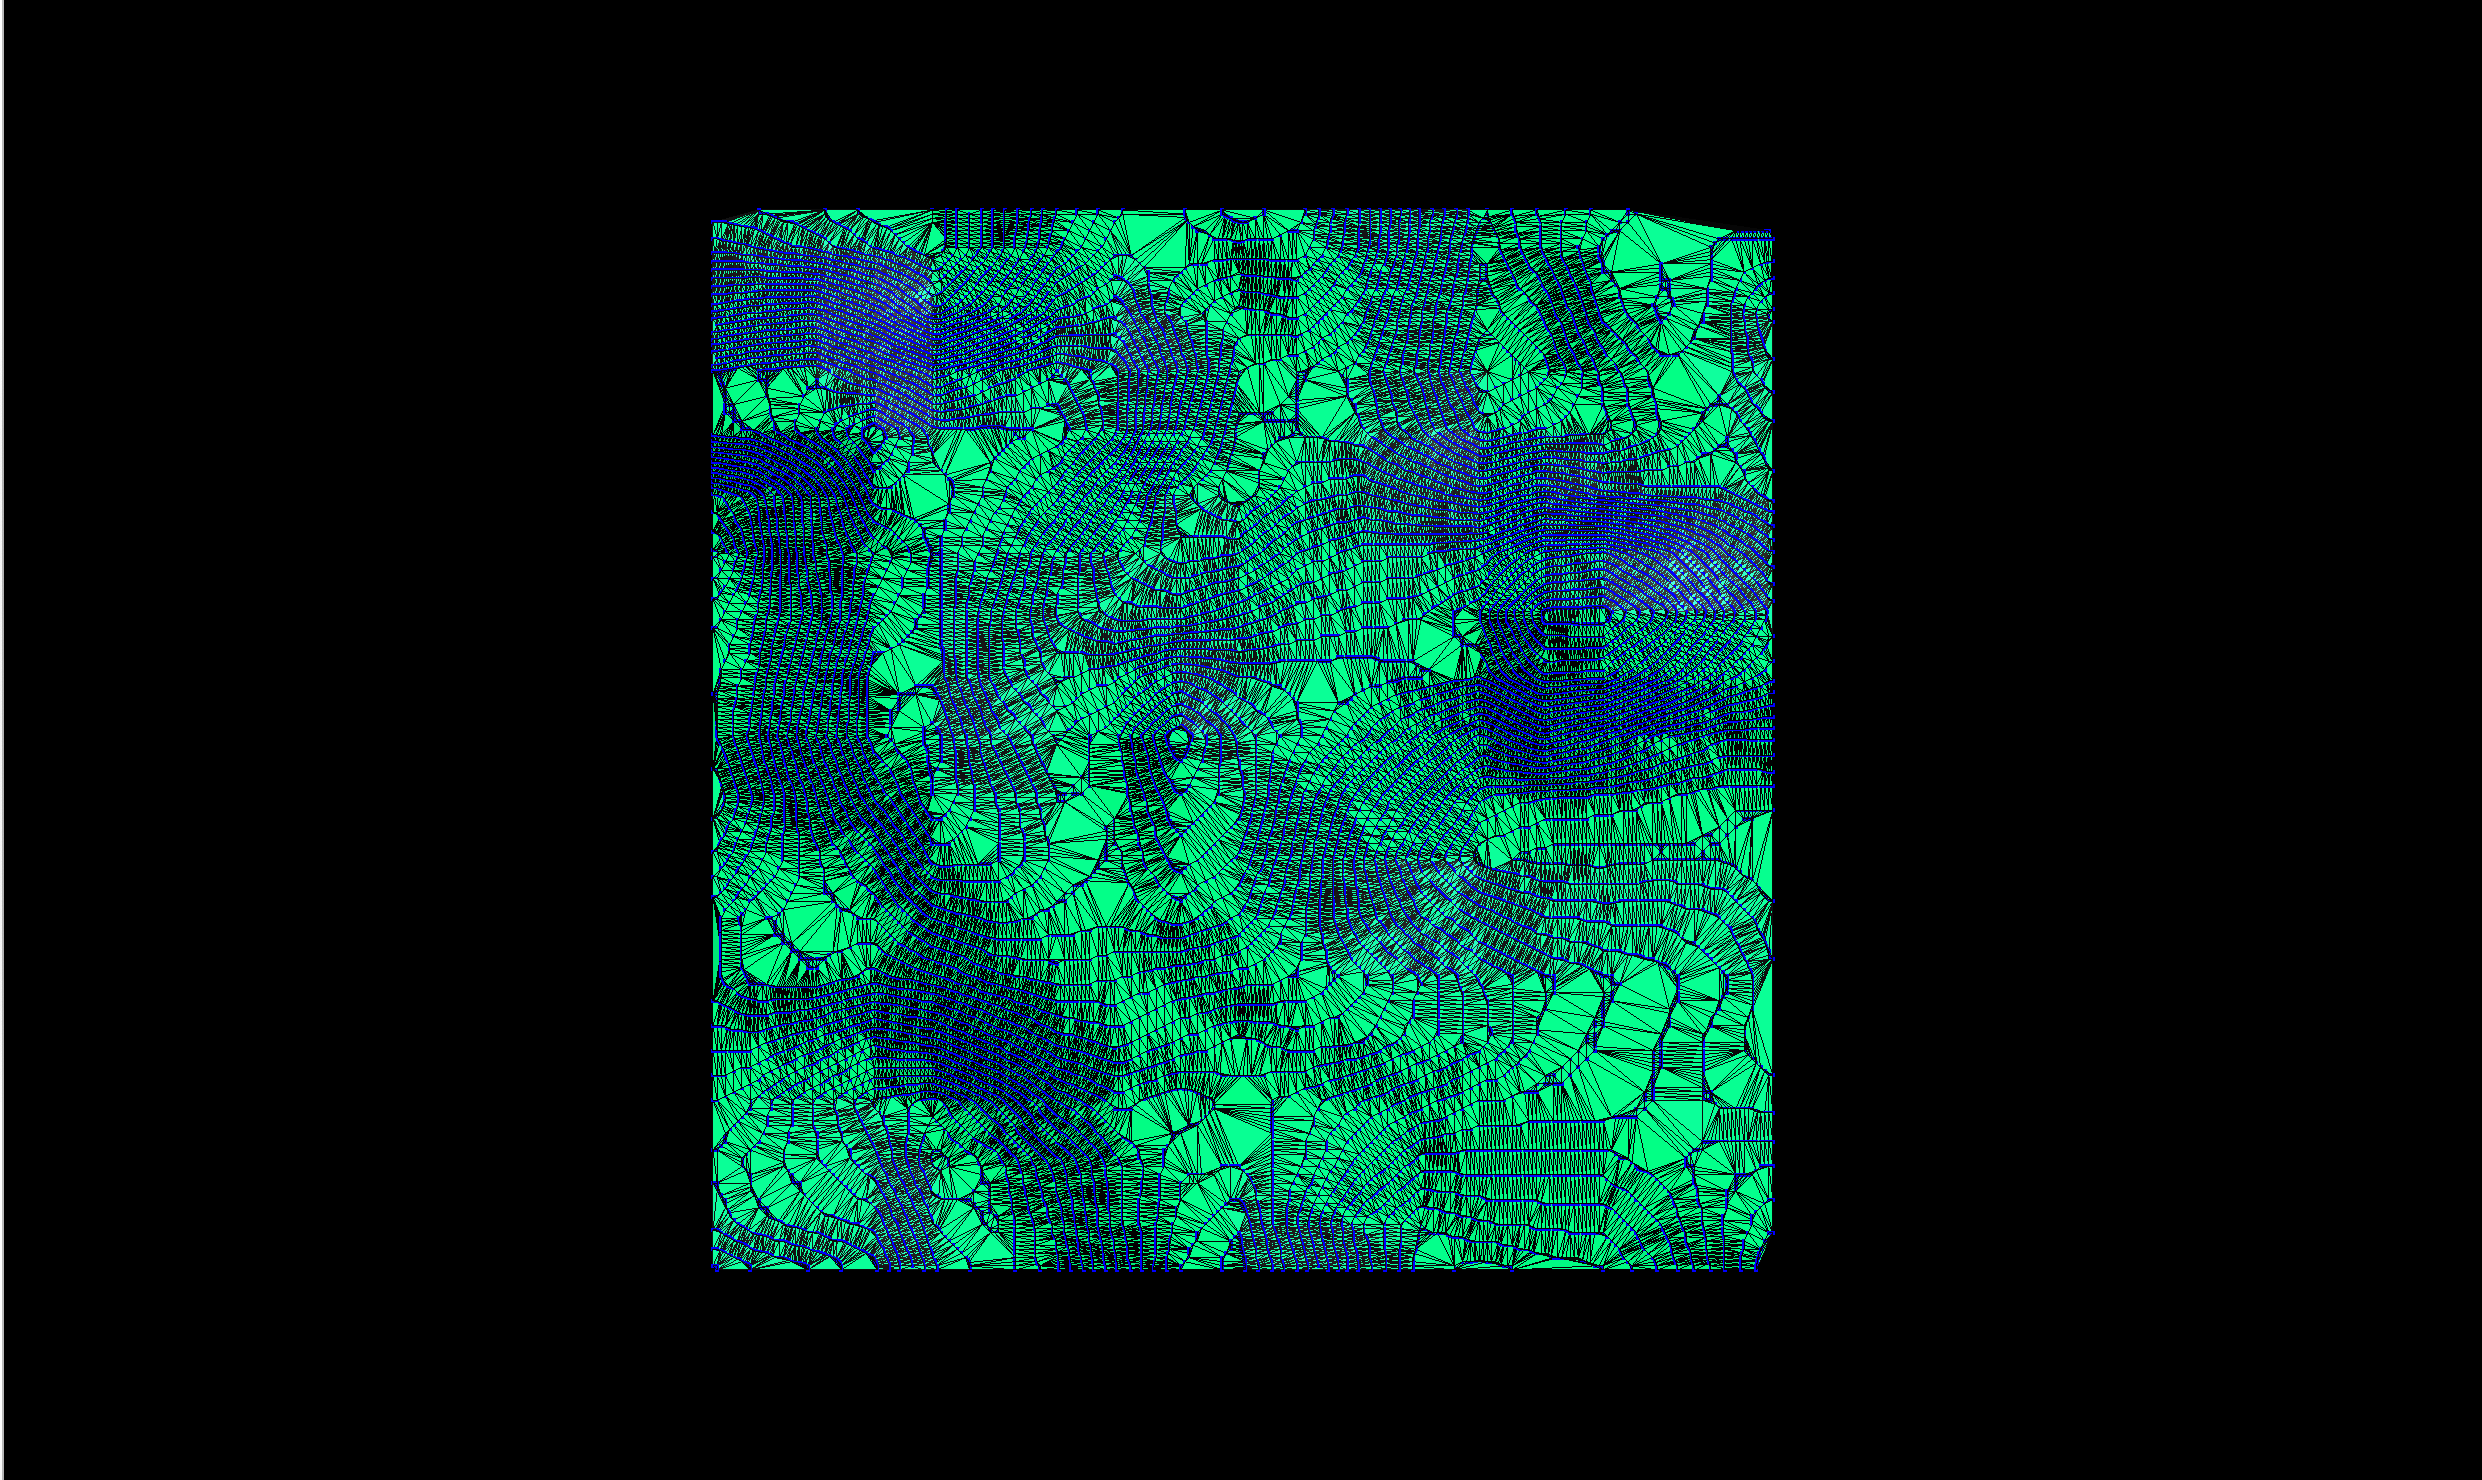
\includegraphics[width=0.8\textwidth]{images/constrained-grenoble-16-1.png}
    \captionsetup{font={scriptsize}}
    \caption{3D mesh after re-triangulation (GPS data zoom 16)}
\end{figure}
\end{frame}

\begin{frame}{Results}
  \begin{figure}[H]
    \centering
    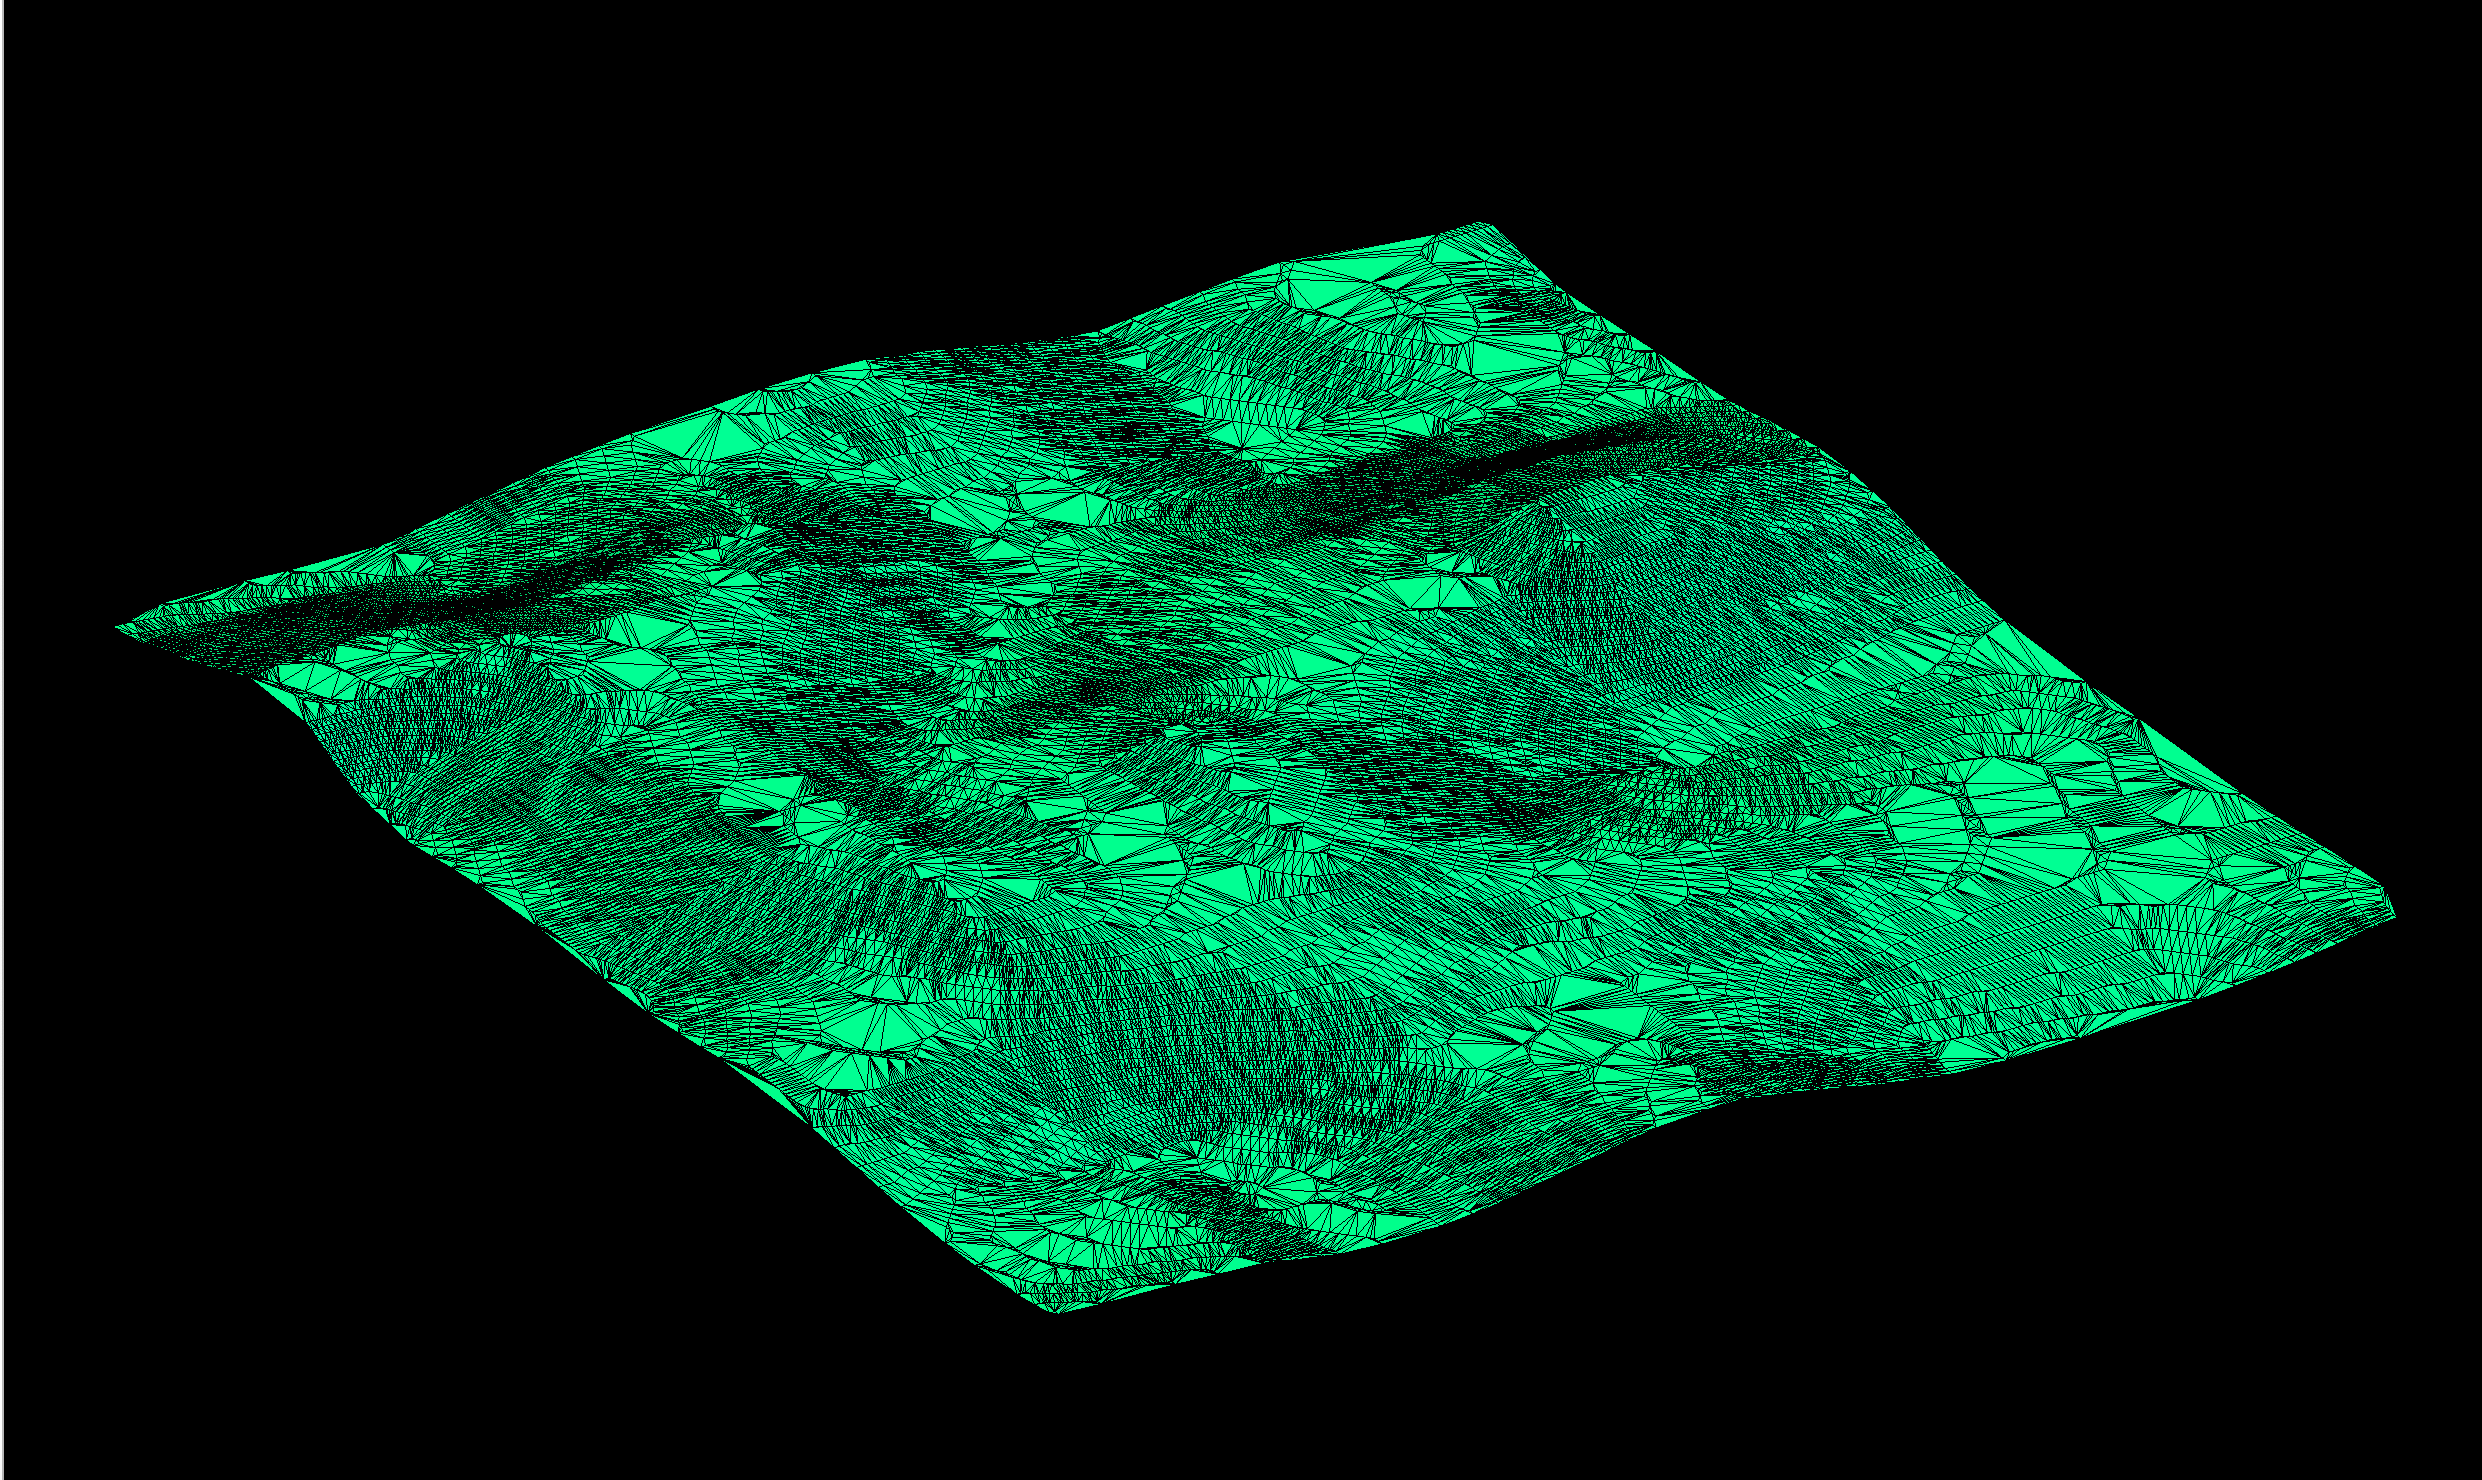
\includegraphics[width=0.8\textwidth]{images/constrained-grenoble-16-2.png}
    \captionsetup{font={scriptsize}}
    \caption{3D mesh after re-triangulation (GPS data zoom 16) side view}
\end{figure}
\end{frame}

\begin{frame}{Results}
  \centering
  \Large
  $(x, y) = (16904, 11763)$ at zoom level $15$
  \begin{figure}[H]
    \centering
    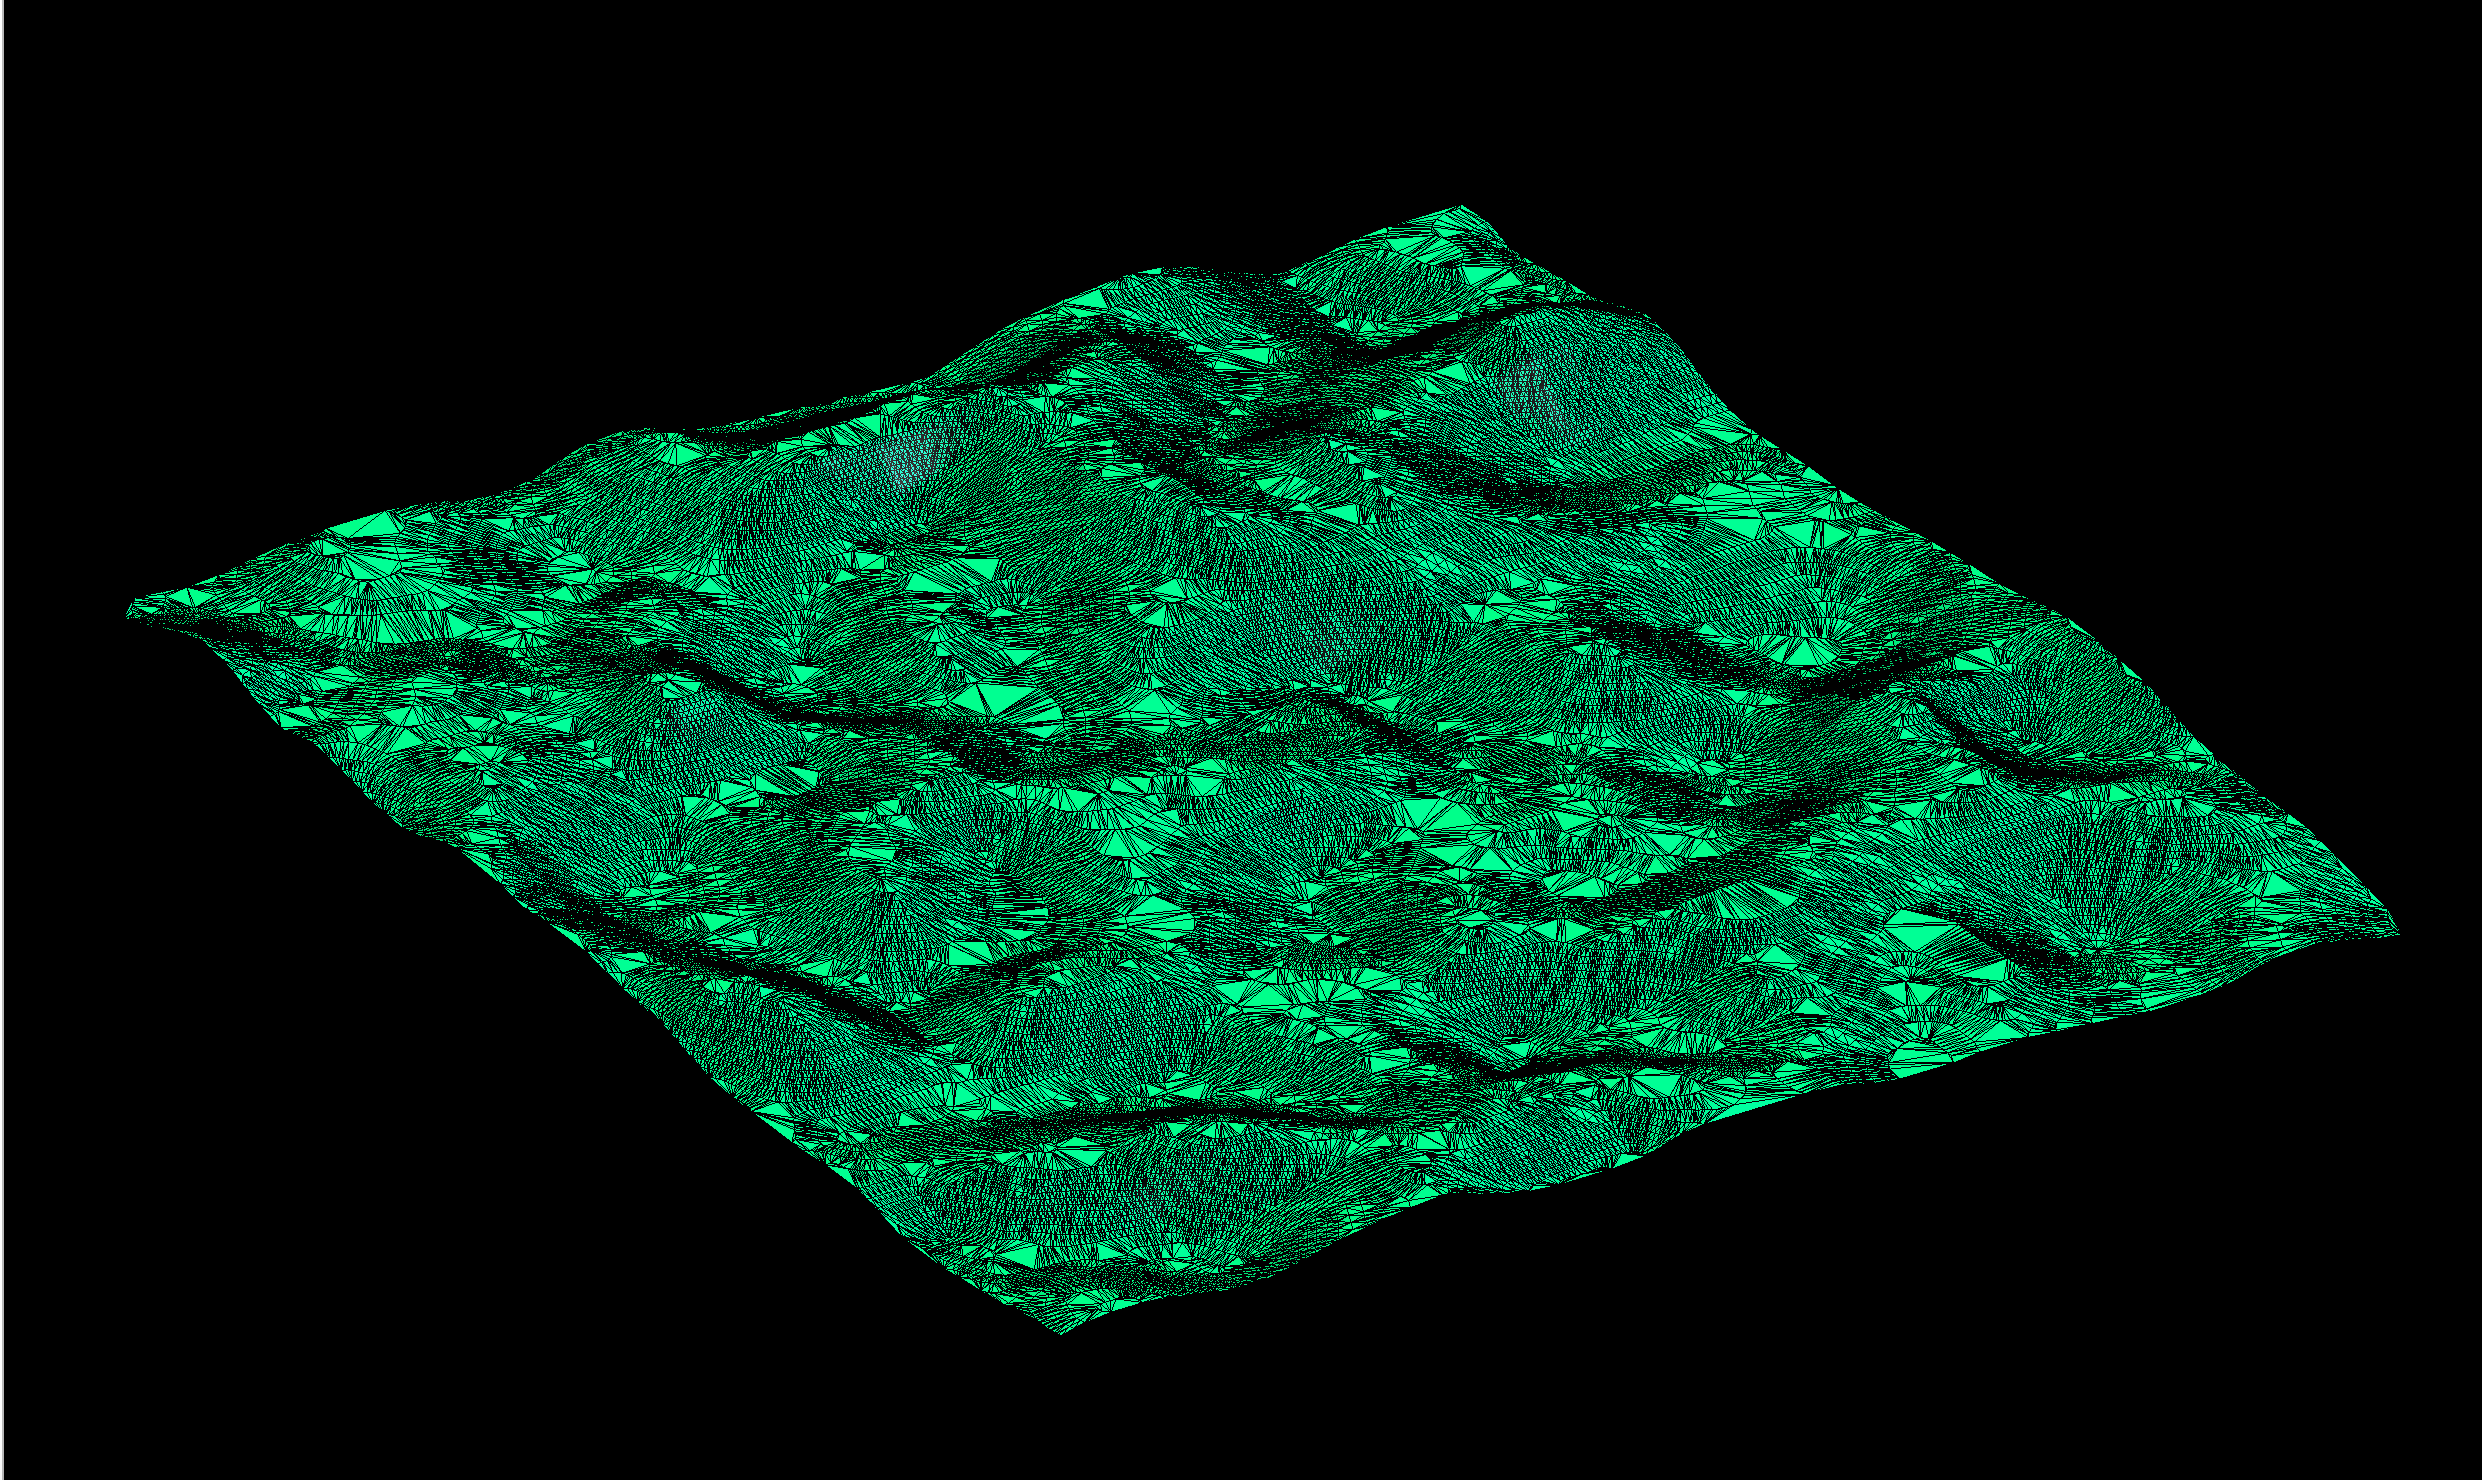
\includegraphics[width=0.8\textwidth]{images/constrained-grenoble-15-1.png}
    \captionsetup{font={scriptsize}}
    \caption{3D mesh after re-triangulation (GPS data zoom 15)}
\end{figure}
\end{frame}

\begin{frame}{Results}
  \begin{figure}[H]
    \centering
    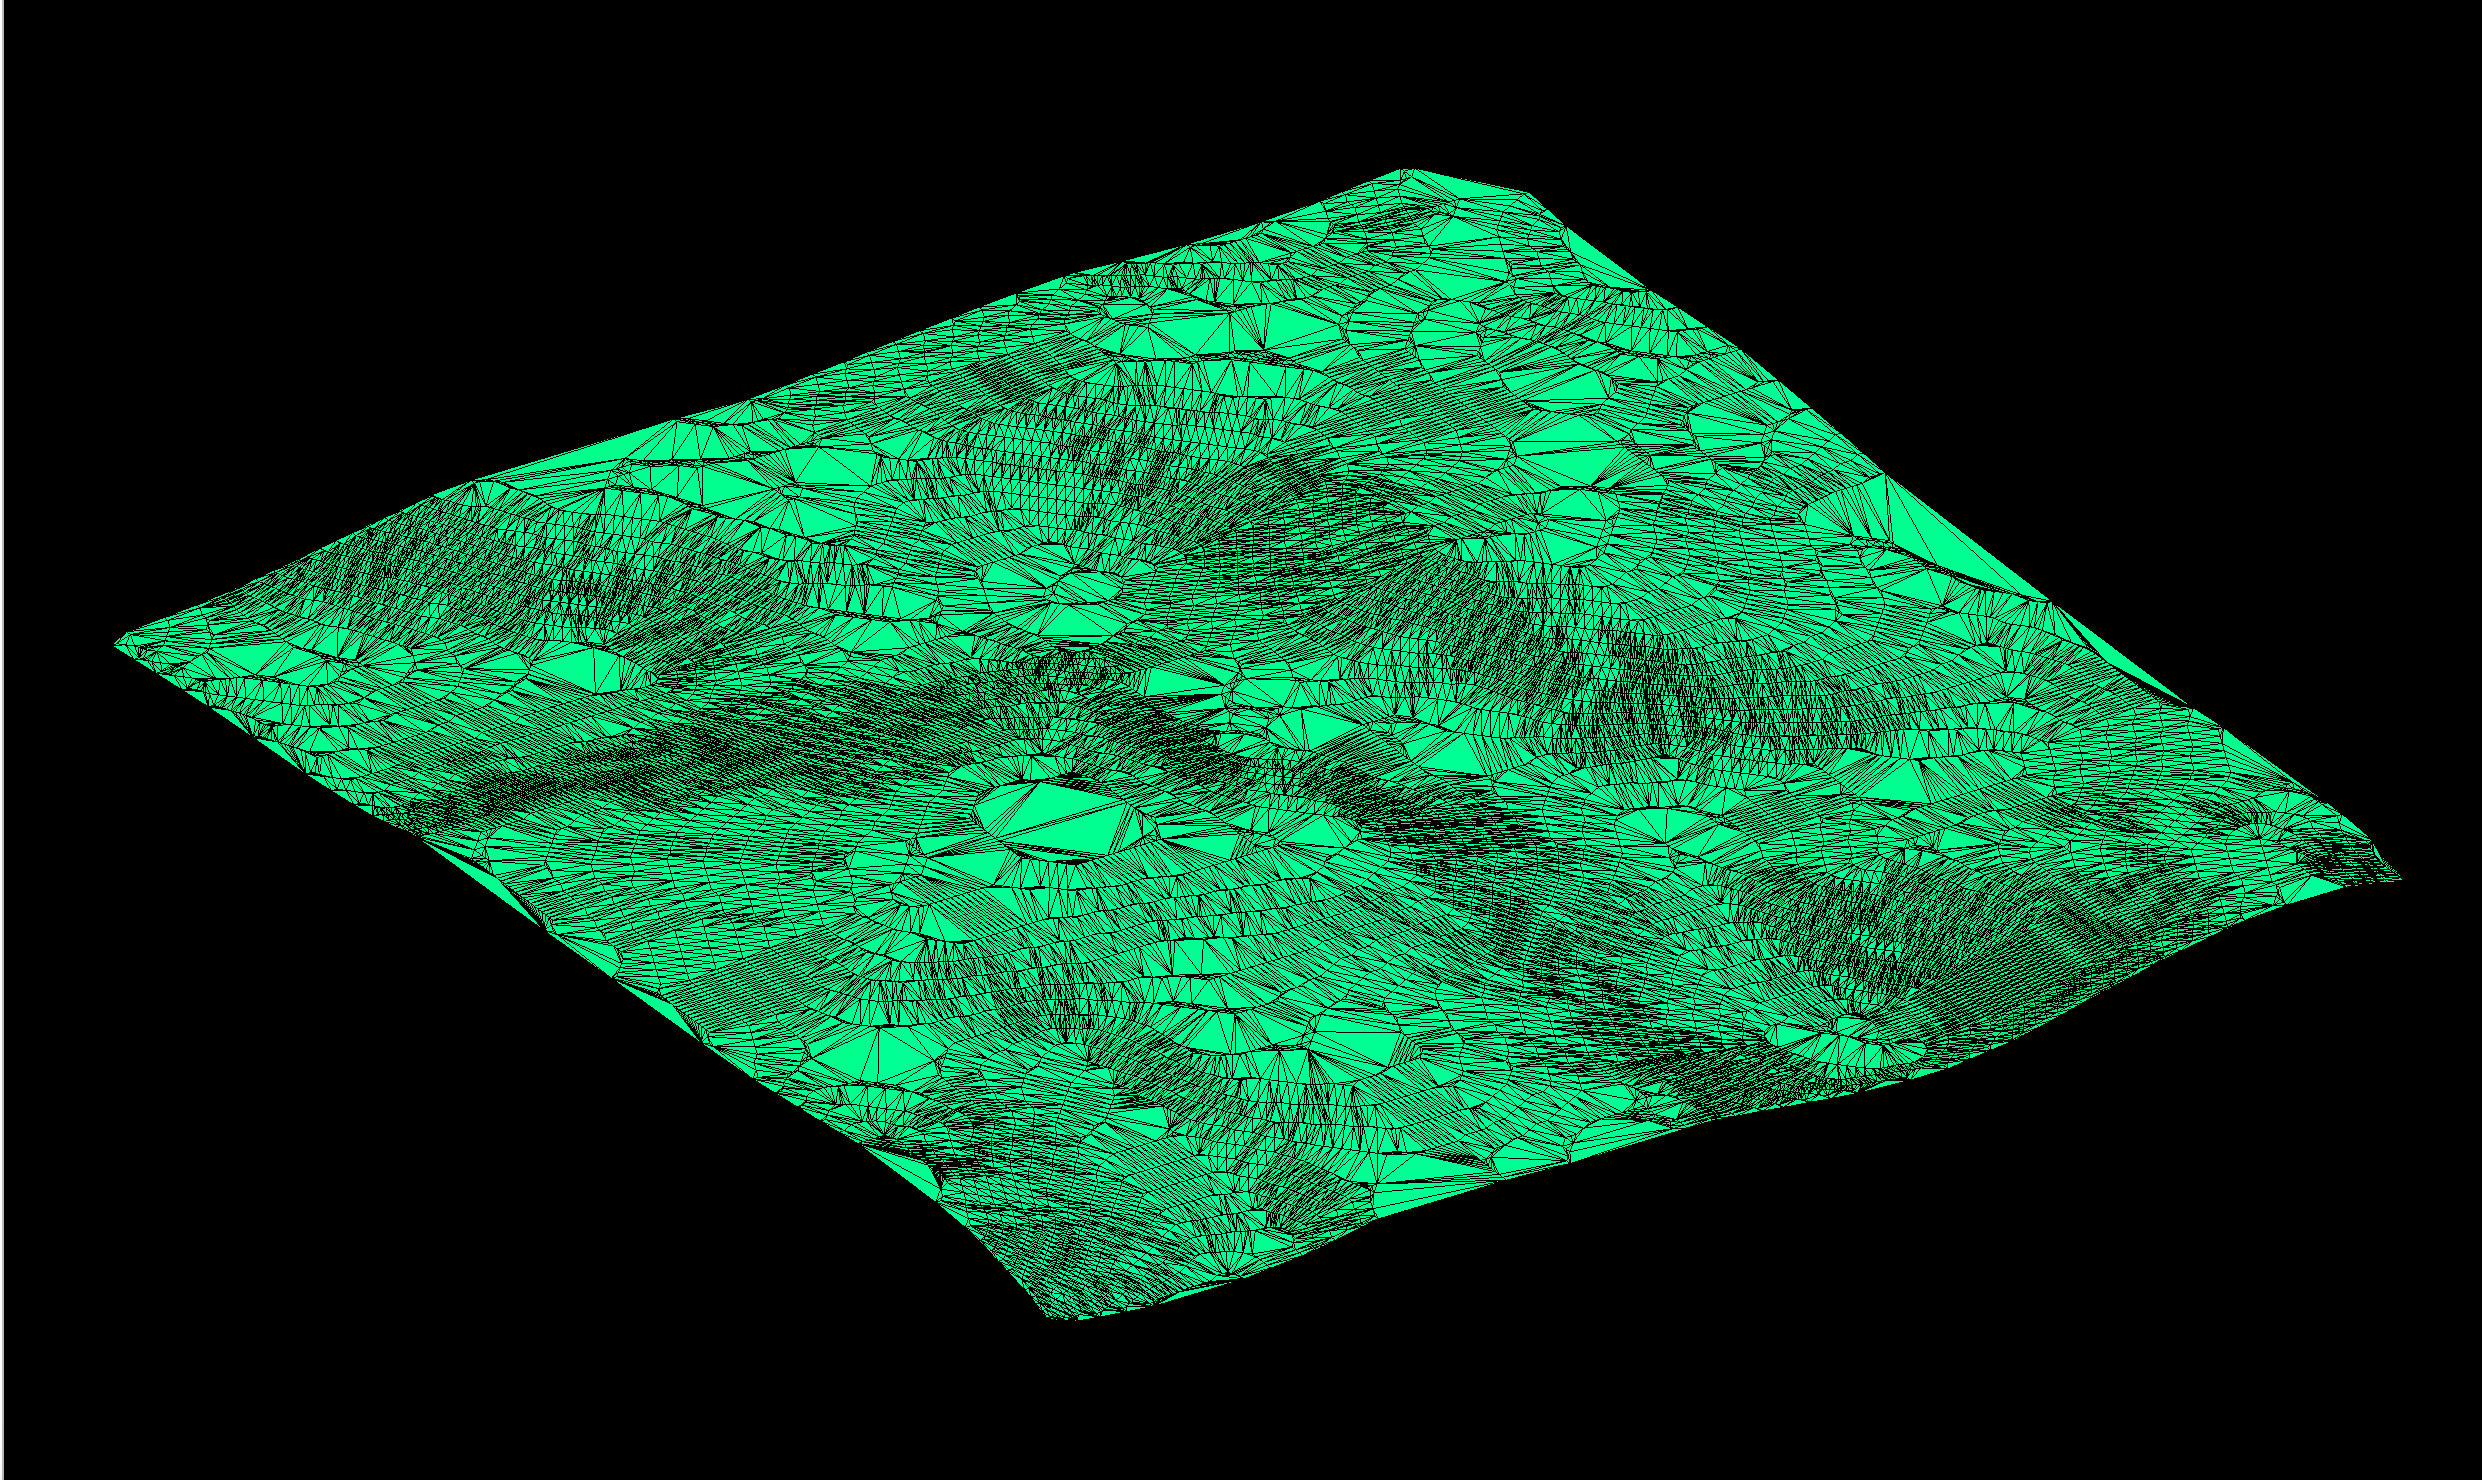
\includegraphics[width=0.8\textwidth]{images/constrained-strasbourg-16.png}
    \captionsetup{font={scriptsize}}
    \caption{3D mesh after re-triangulation (GPS data Strasbourg zoom 16)}
\end{figure}
\end{frame}

\begin{frame}{Results}
  \begin{figure}[H]
    \centering
    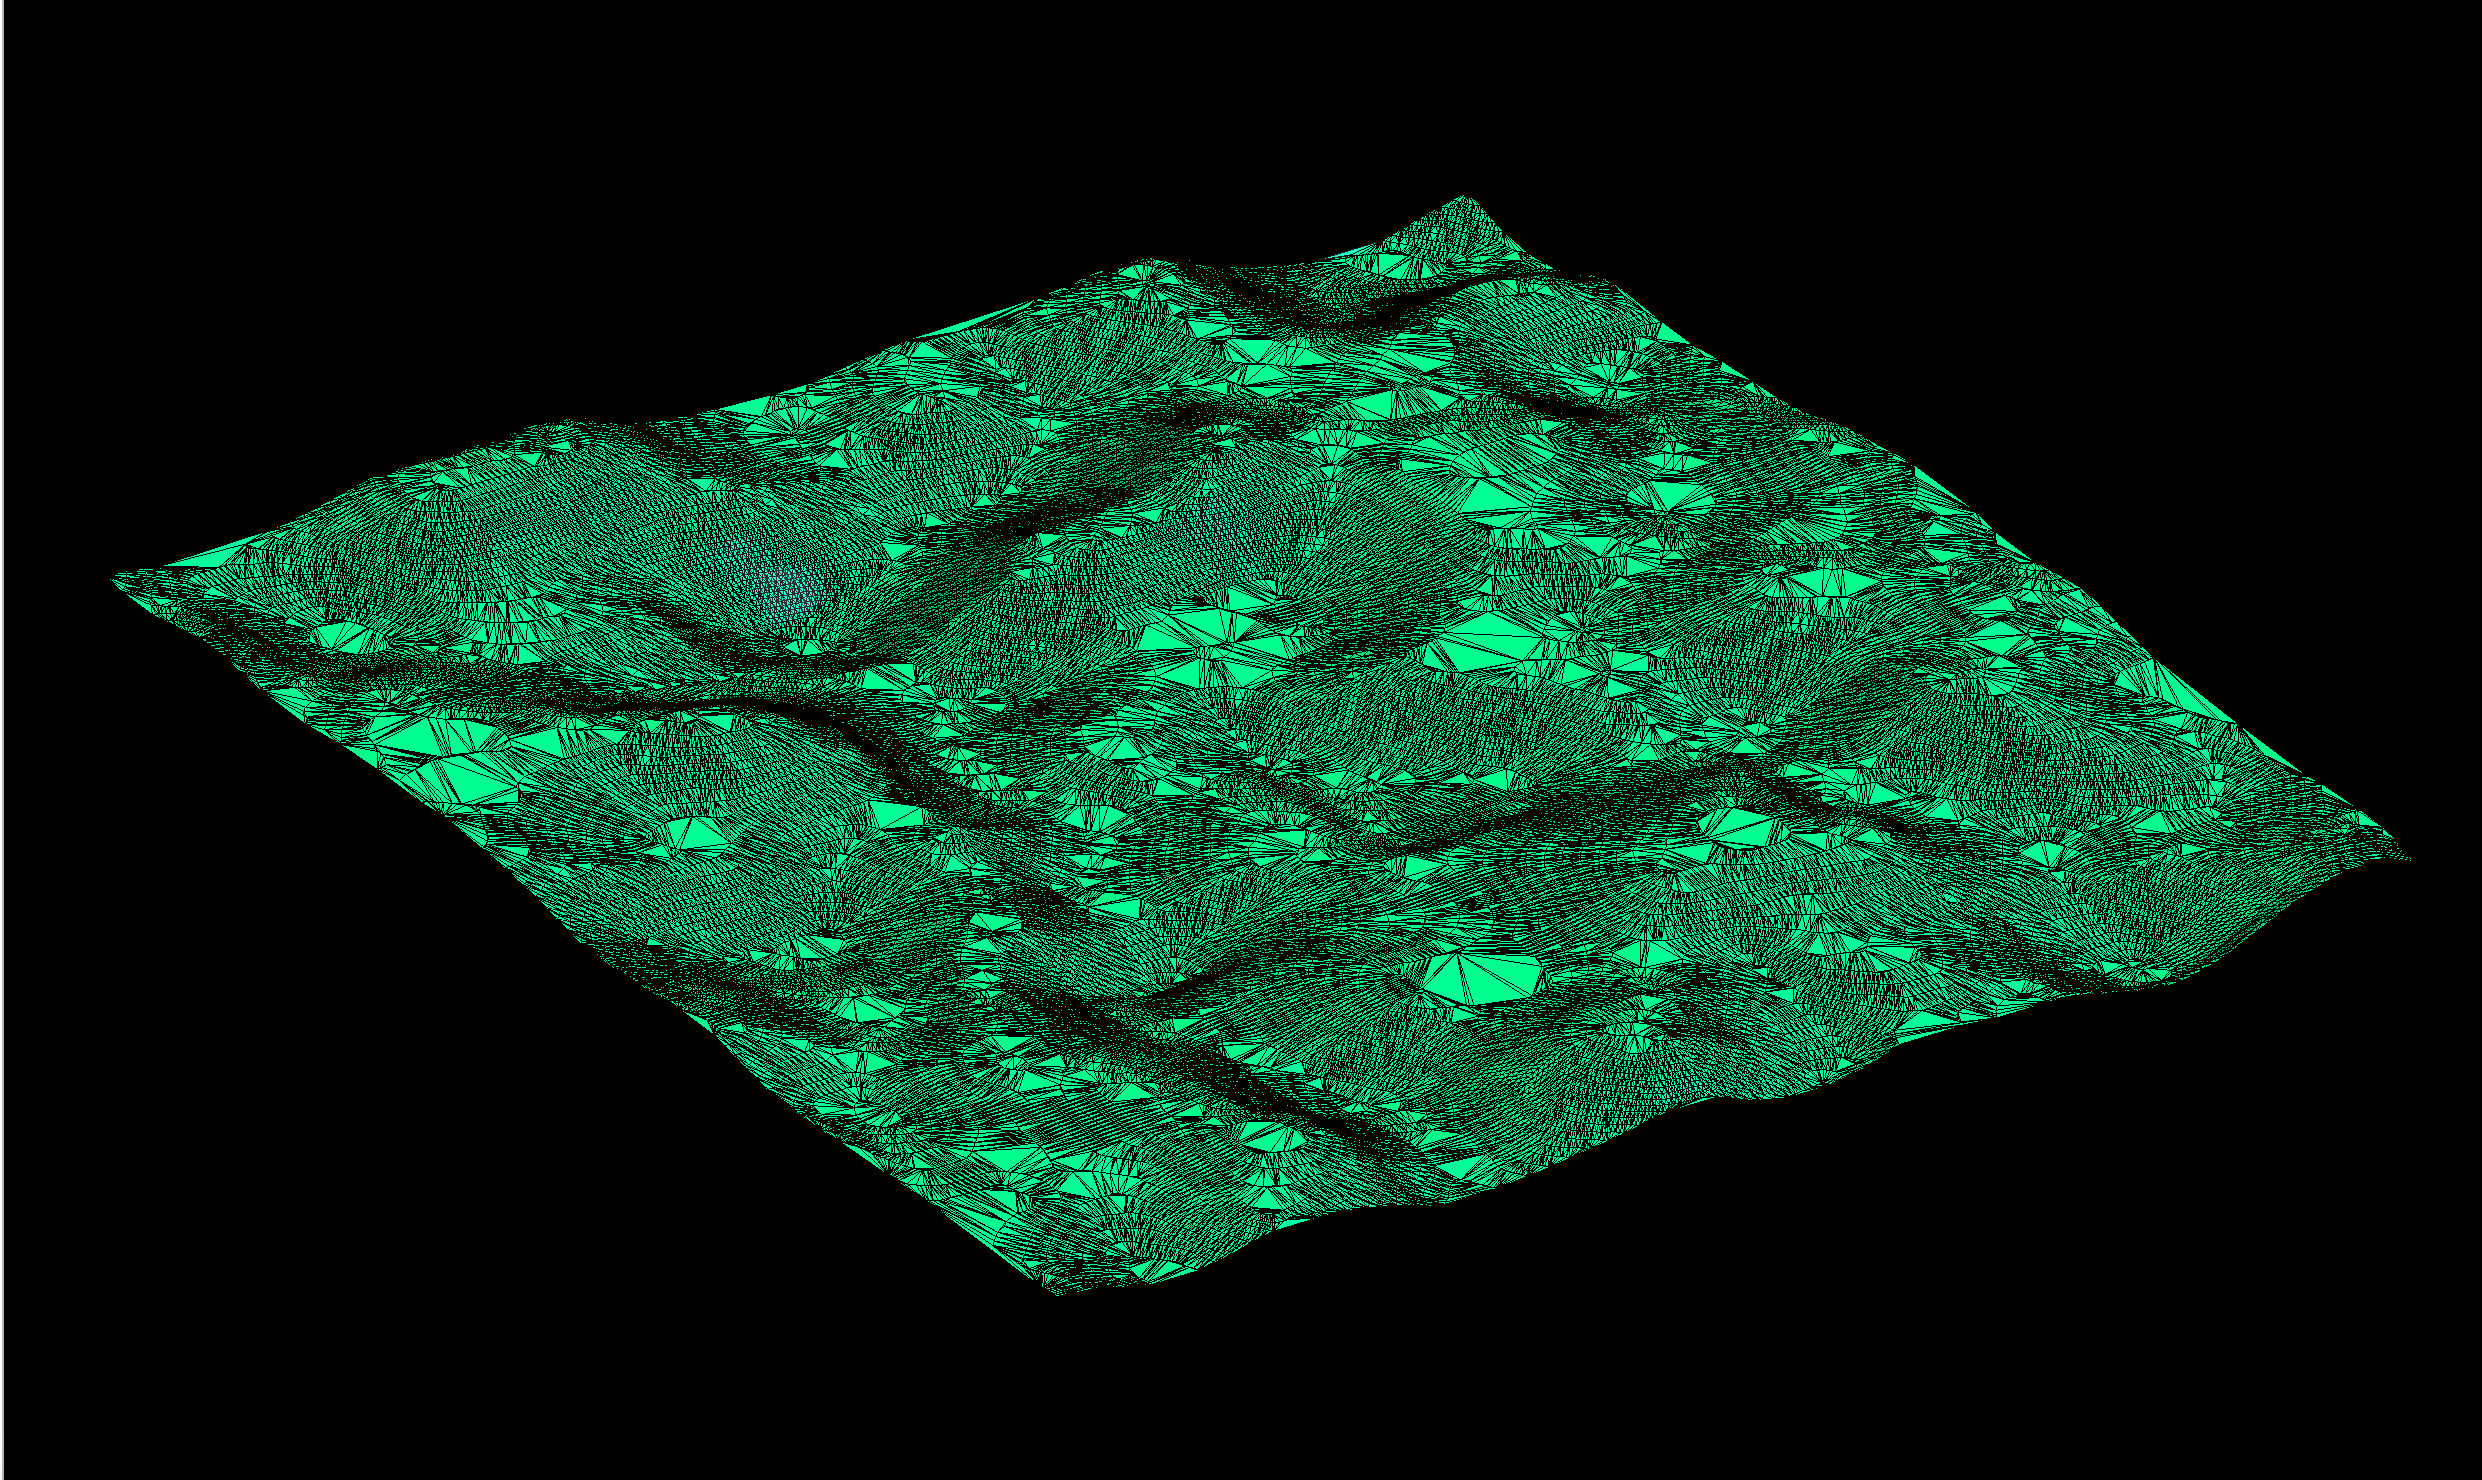
\includegraphics[width=0.8\textwidth]{images/constrained-strasbourg-15.png}
    \captionsetup{font={scriptsize}}
    \caption{3D mesh after re-triangulation (GPS data Strasbourg zoom 15)}
\end{figure}
\end{frame}

\begin{frame}{Prospects: Handling and merging multiple tiles}
  \begin{figure}[H]
    \centering
    \begin{minipage}{0.4\textwidth}
      \centering
      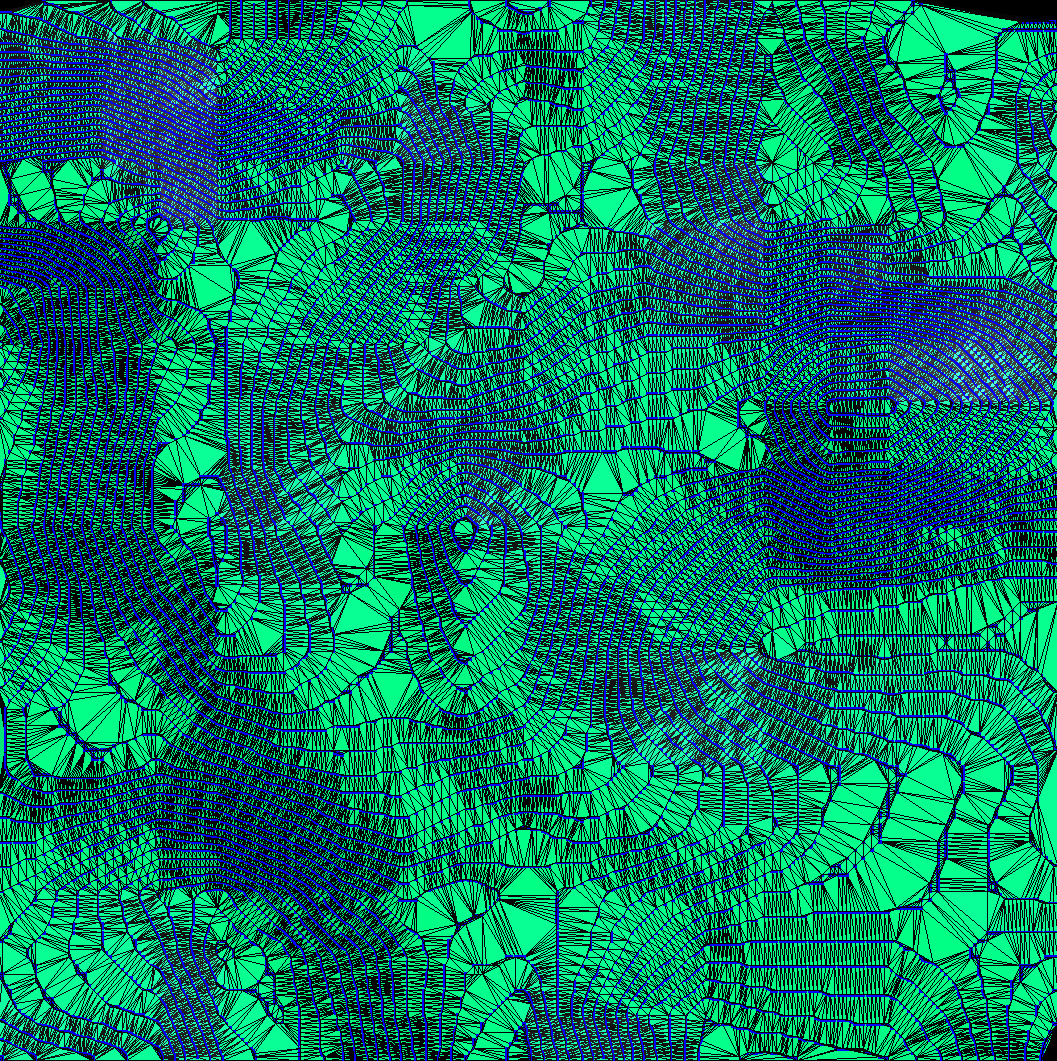
\includegraphics[width=0.7\textwidth]{images/1.png}
      \captionsetup{font={scriptsize}}
      \caption{(33809, 23527)}
    \end{minipage}
    \begin{minipage}{0.4\textwidth}
      \centering
      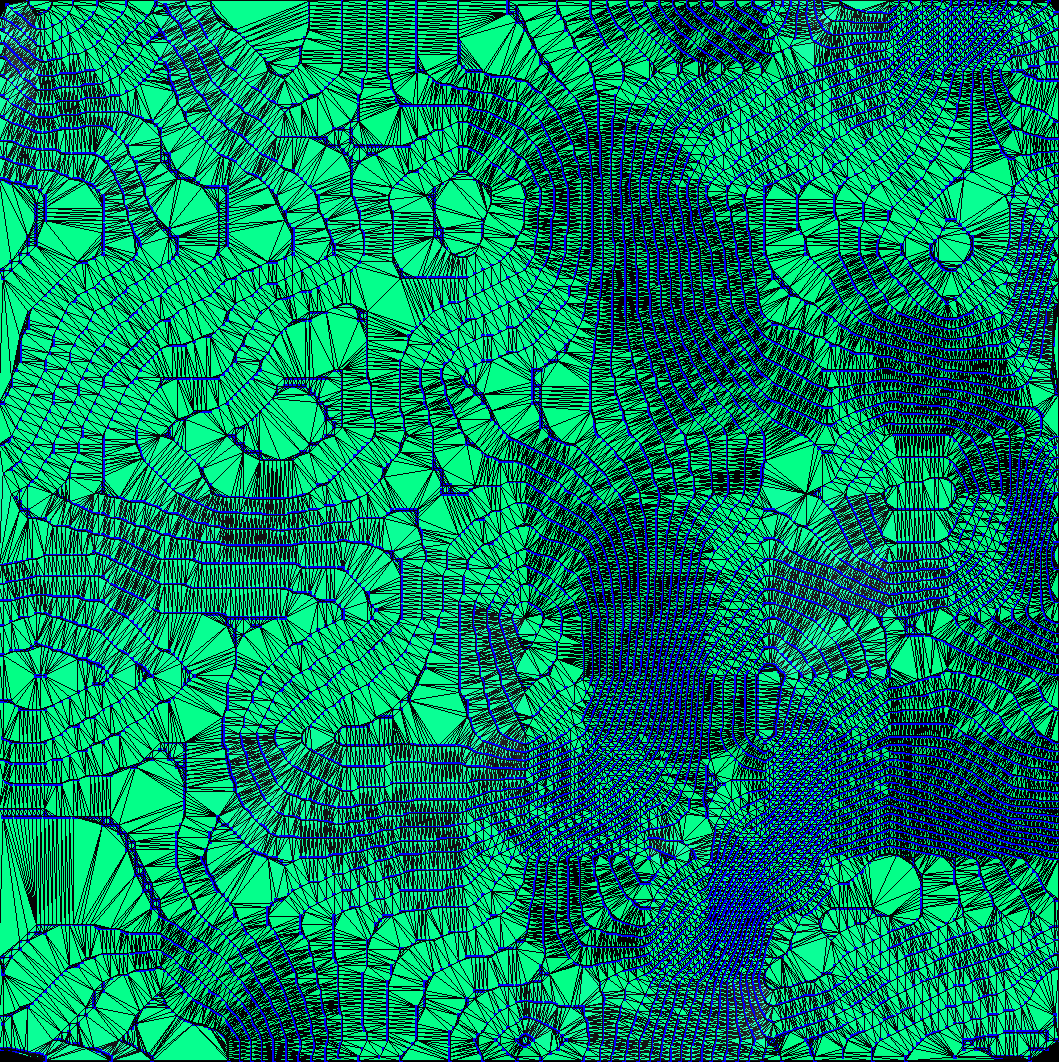
\includegraphics[width=0.7\textwidth]{images/2.png}
      \captionsetup{font={scriptsize}}
      \caption{(33810, 23527)}
    \end{minipage}
  \end{figure}

  \begin{figure}[H]
    \centering
    \begin{minipage}{0.4\textwidth}
      \centering
      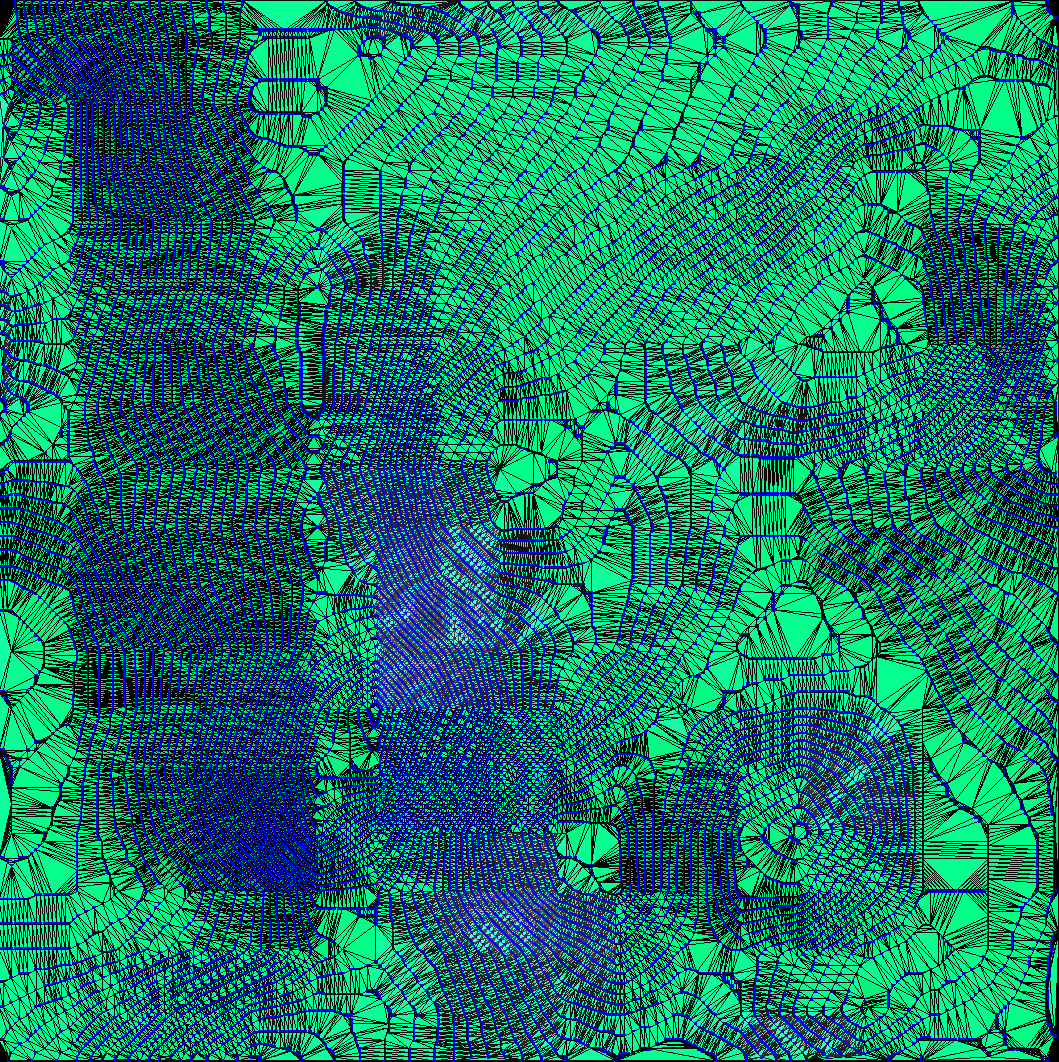
\includegraphics[width=0.7\textwidth]{images/3.png}
      \captionsetup{font={scriptsize}}
      \caption{(33809, 23528)}
    \end{minipage}
    \begin{minipage}{0.4\textwidth}
      \centering
      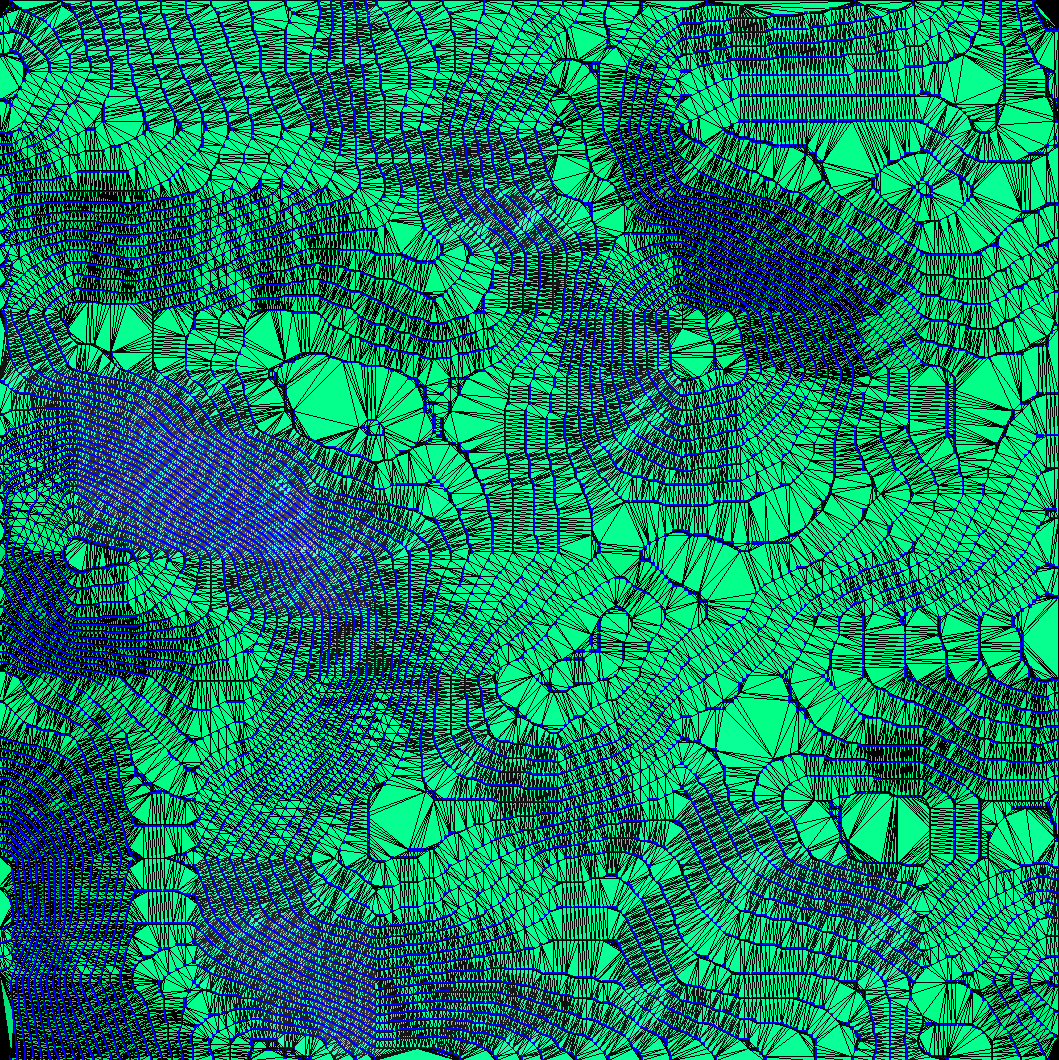
\includegraphics[width=0.7\textwidth]{images/4.png}
      \captionsetup{font={scriptsize}}
      \caption{(33810, 23528)}
    \end{minipage}
  \end{figure}
\end{frame}

\begin{frame}{Prospects: Handling and merging multiple tiles}
  \begin{figure}[H]
    \centering
    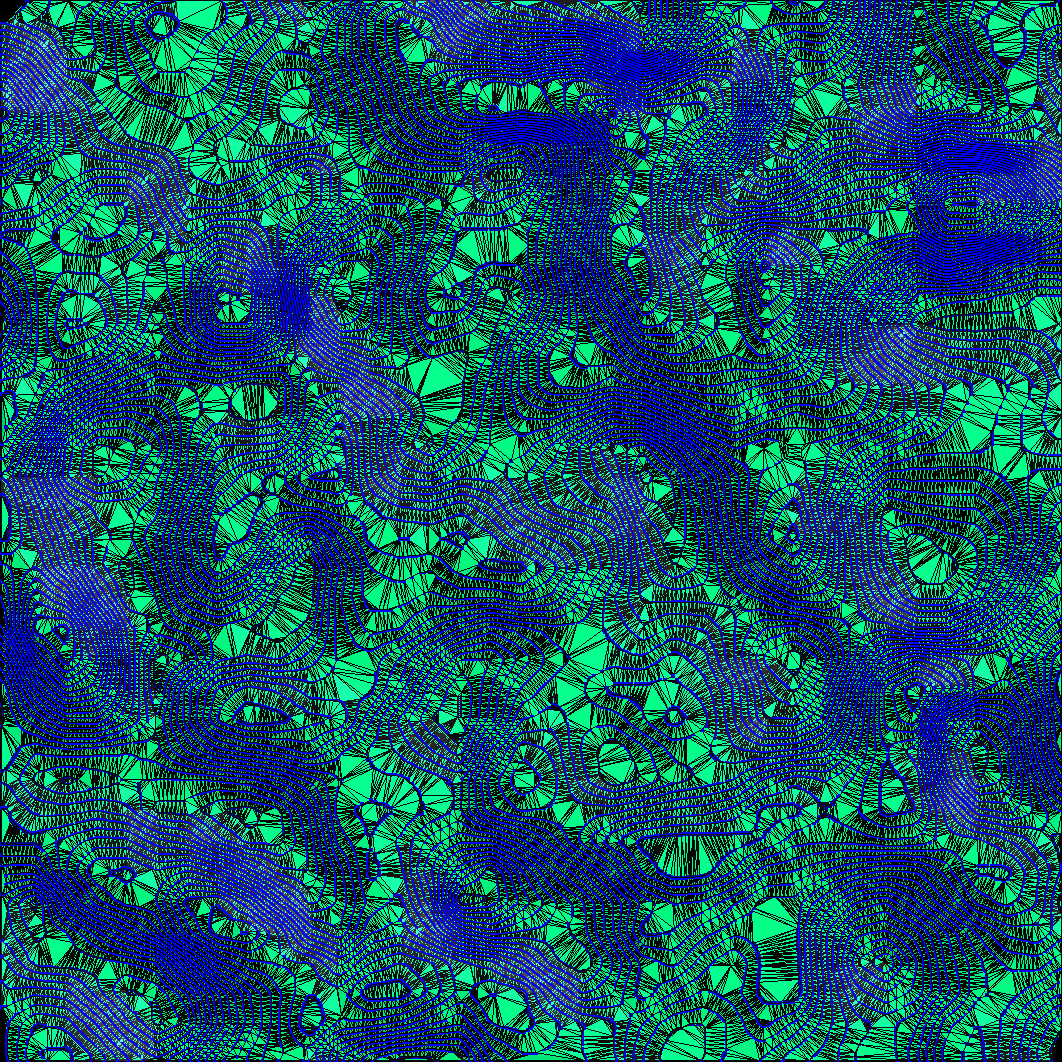
\includegraphics[width=0.65\textwidth]{images/5.png}
    \captionsetup{font={scriptsize}}
    \caption{Resultig merged tile}
  \end{figure}
\end{frame}

\begin{frame}{Prospects: Mesh refinement}
  \begin{figure}[H]
    \centering
    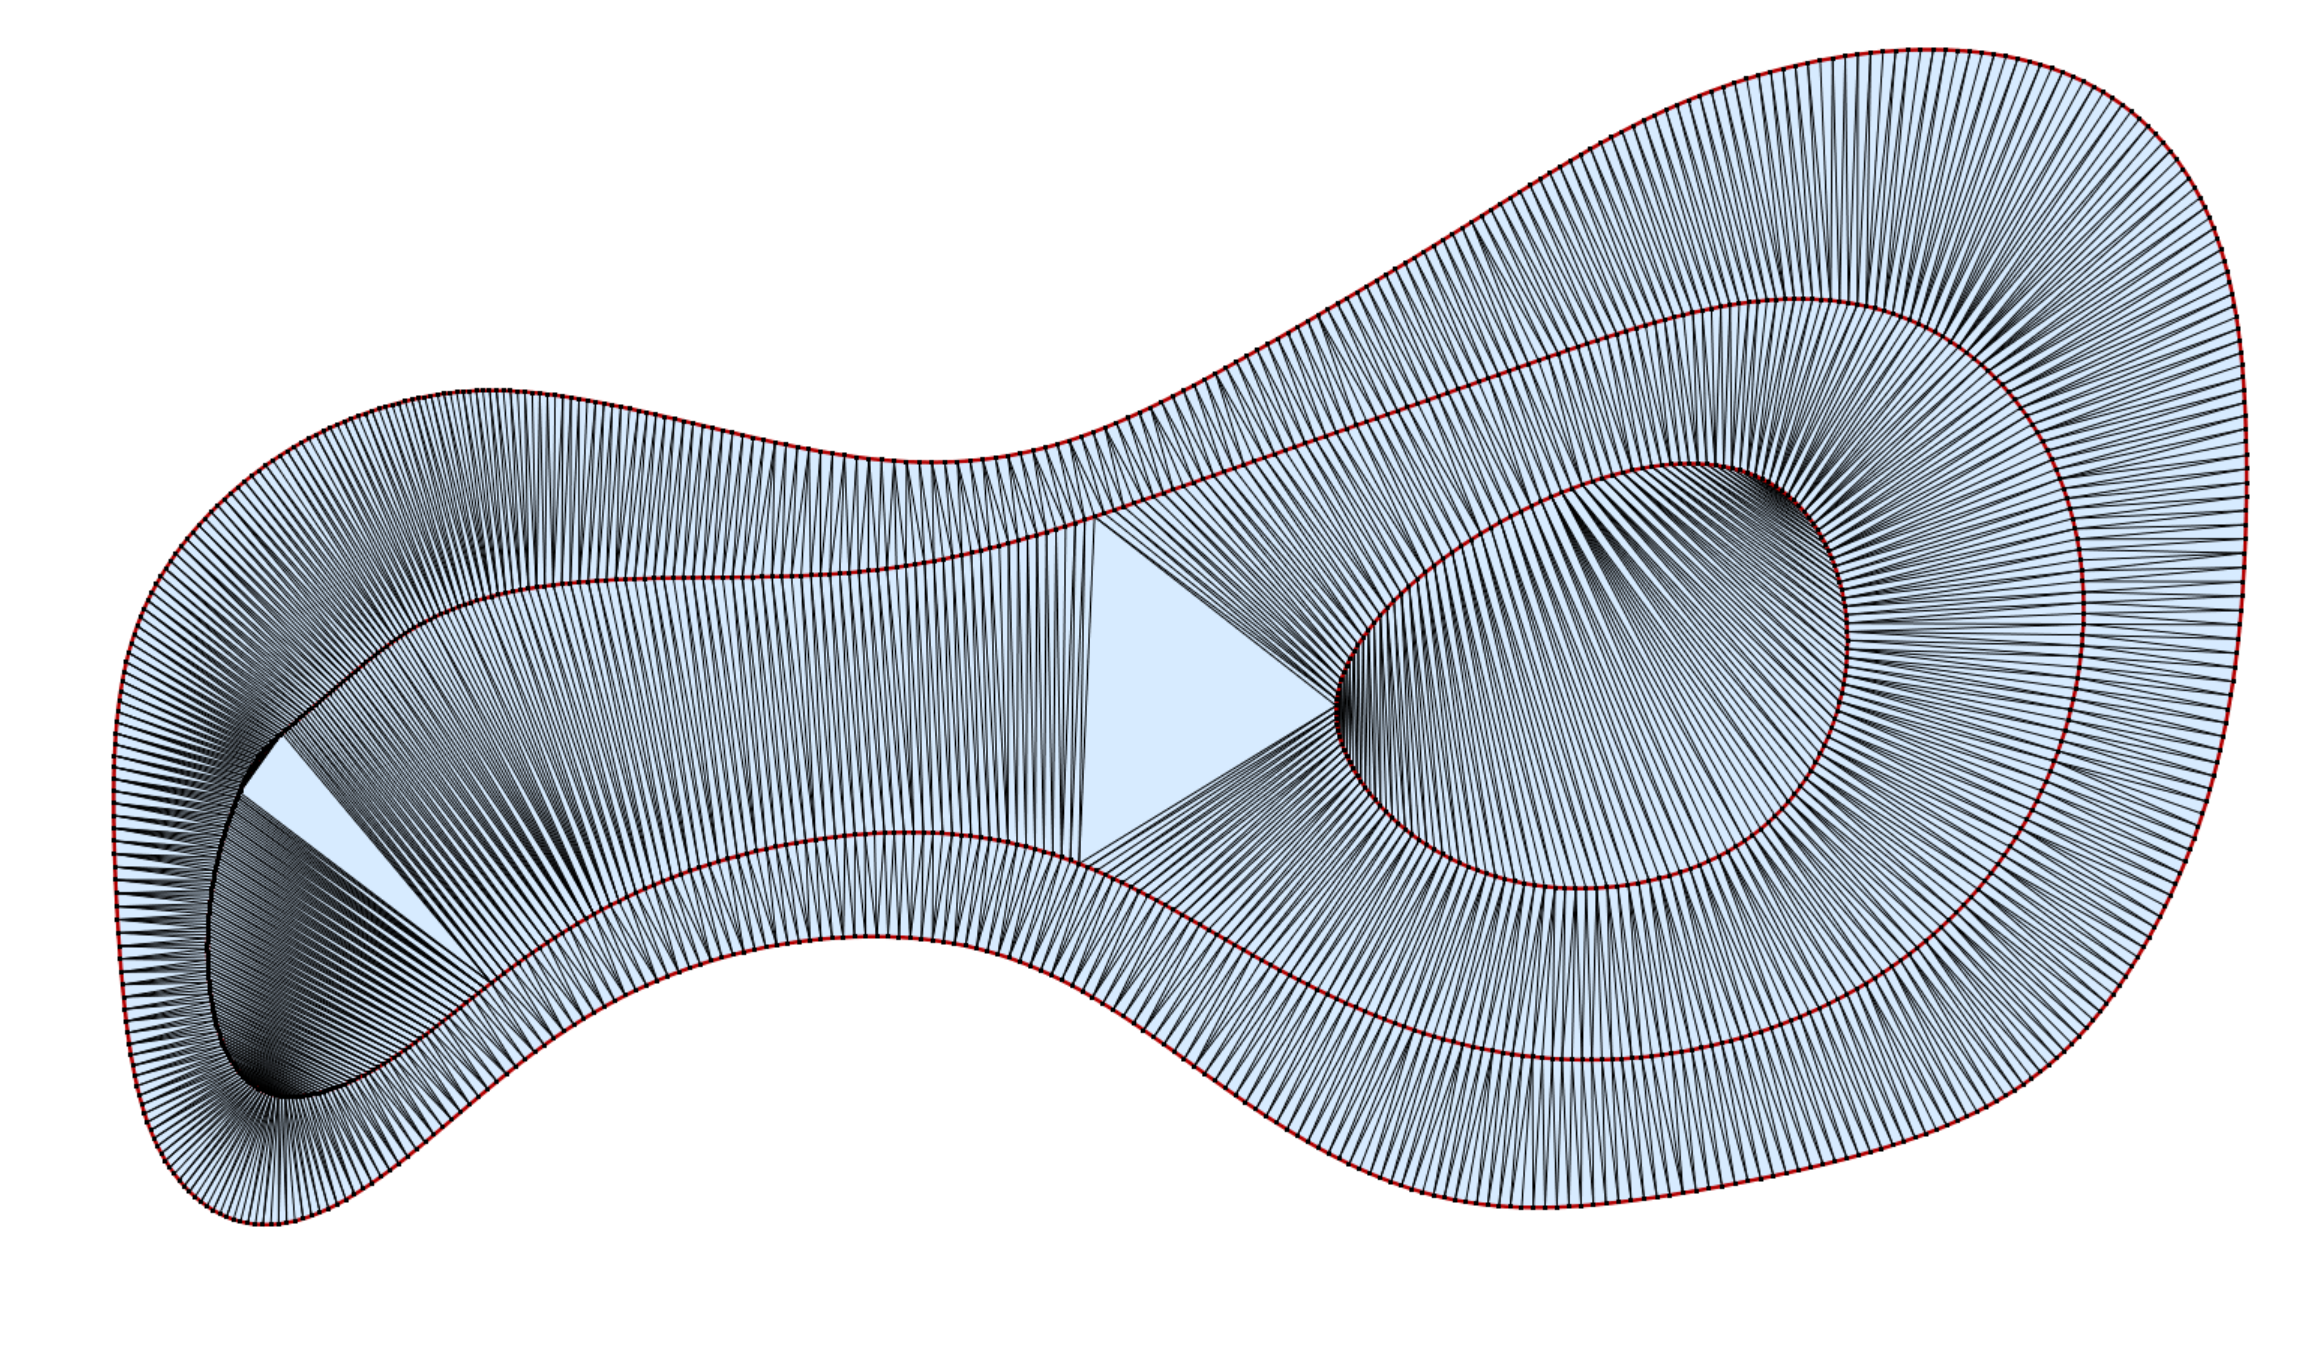
\includegraphics[width=0.9\textwidth]{images/mesh.png}
    \captionsetup{font={scriptsize}}
    \caption{Mesh constrained to contour lines}
\end{figure}
\end{frame}

\begin{frame}{Prospects: Mesh refinement}
  \begin{figure}[H]
    \centering
    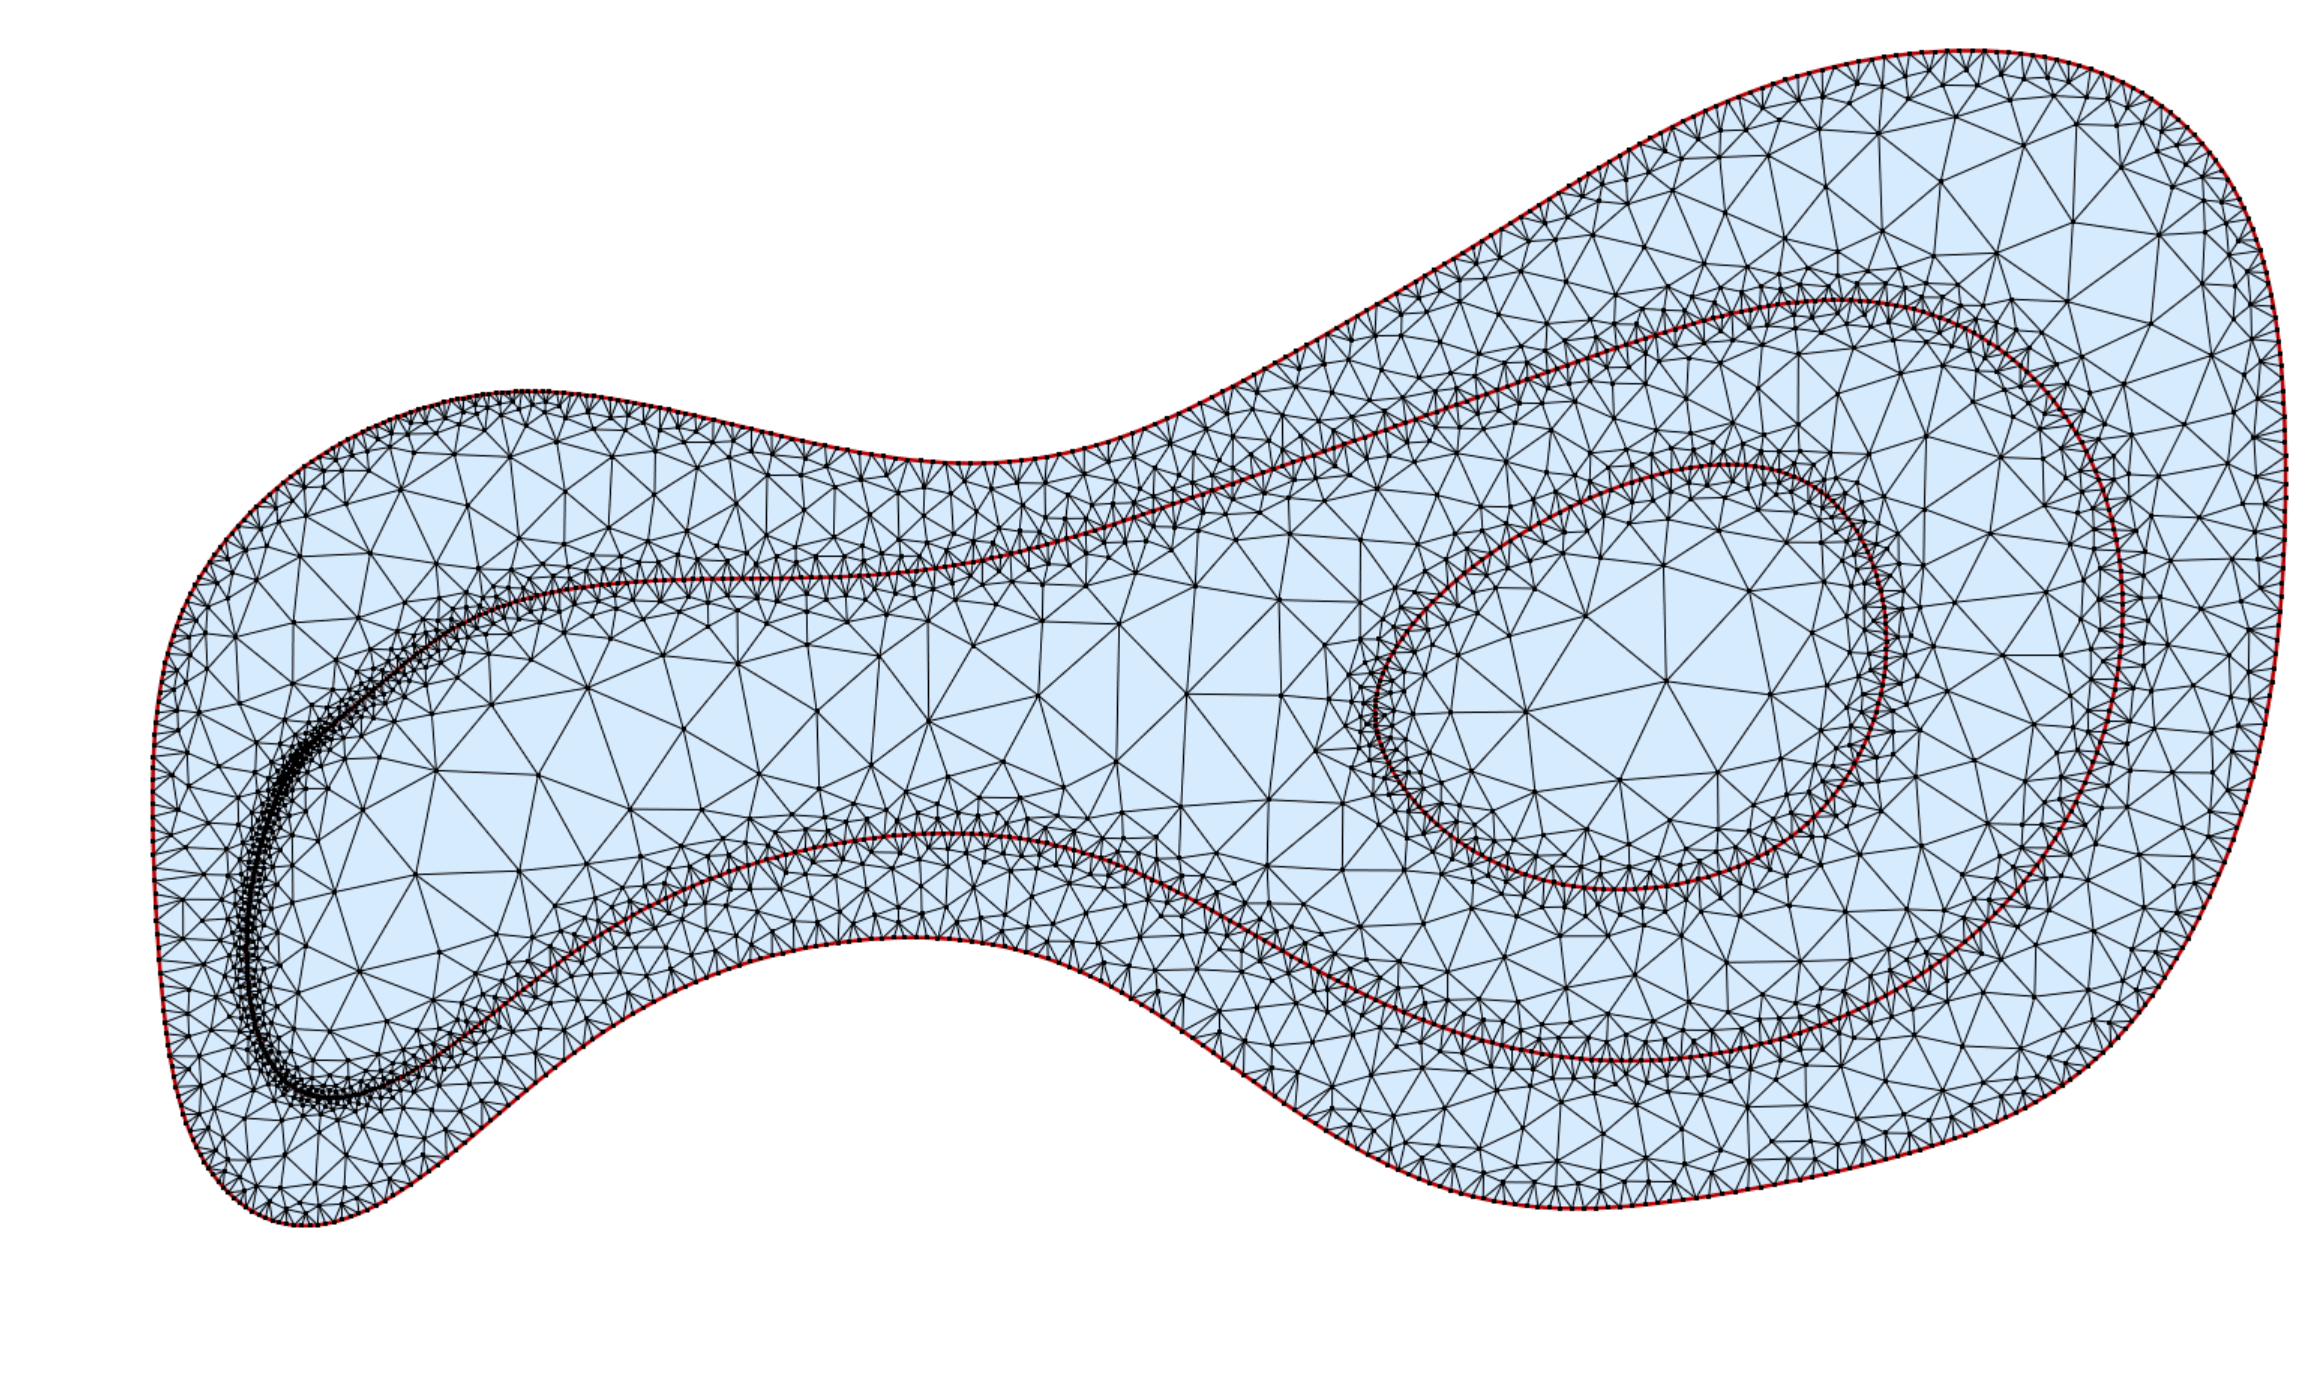
\includegraphics[width=0.9\textwidth]{images/mesh-refined.png}
    \captionsetup{font={scriptsize}}
    \caption{Mesh refined}
\end{figure}
\end{frame}

\begin{frame}{Prospects: Parallelization}
  \Large
  \begin{itemize}
    \item \textbf{Parallel processing} of \textbf{multiple tiles}
    \item \textbf{Parallelizing mesh generation}
    \item \textbf{Parallel tile merging}
  \end{itemize}
\end{frame}

\begin{frame}{Prospects: Urban elements integration}
  \Large
  \begin{itemize}
    \item \textbf{Integrating urban} elements with \textbf{terrain models}
    \vspace{2em}
    \item \textbf{\textcolor{red}{Detailed 3D model}} of the \textbf{urban environment}
  \end{itemize}
\end{frame}

\begin{frame}{Conclusion}
  \Large
  Flexible \textbf{terrain} generation:
  \vspace{1em}
  \begin{itemize}
    \item \textbf{LambdaGenerator}
    \item \textbf{GpsGenerator}
  \end{itemize}
\end{frame}

\begin{frame}{Conclusion}
  \Large
  \textbf{Contour lines} generation:
  \vspace{1em}
  \begin{itemize}
      \item \textbf{ContourConstraint}
  \end{itemize}
\end{frame}

\begin{frame}{Conclusion}
  \Large
  \textbf{Triangulation}:
  \vspace{1em}
  \begin{itemize}
    \item \textbf{triangulateAssembledMesh}
  \end{itemize}
\end{frame}

\begin{frame}{Conclusion}
  \Large
  Framework developed provides foundation:
  \vspace{1em}
  \begin{itemize}
    \item \textbf{Future developments} and \textbf{applications}
    \item \textbf{Sustainable urban development} and \textbf{environmental conservation}
  \end{itemize}
\end{frame}

\begin{frame}{The end}
  \Large
  \centering
  \textbf{Thank you all for your attention!}
\end{frame}

\nocite{*}
\bibliographystyle{unsrt}
\bibliography{references}

\end{document}